\documentclass[12pt]{article}

% ----------------------------------------------------------------------
% Define external packages, language, margins, fonts, new commands 
% and colors
% ----------------------------------------------------------------------
\usepackage[utf8]{inputenc} % Codification
\usepackage[english]{babel} % Writing idiom

\usepackage{listings}
\usepackage[dvipsnames]{xcolor}
\usepackage[most]{tcolorbox}
\usepackage{float}


\definecolor{codebg}{RGB}{245,245,245}
\definecolor{codeframe}{RGB}{200,200,200}

\lstdefinestyle{CiscoStyle}{
    backgroundcolor=\color{codebg},
    basicstyle=\ttfamily\small,
    keywordstyle=\color{blue},
    commentstyle=\color{gray},
    breaklines=true,
    showstringspaces=false,
    columns=fullflexible
}

\newtcblisting{configbox}{
    listing only,
    colback=codebg,
    colframe=codeframe,
    arc=3mm,
    boxrule=0.5pt,
    left=2mm,
    right=2mm,
    top=1mm,
    bottom=1mm,
    listing options={style=CiscoStyle}
}

\newtcblisting{largeconfigbox}{
    listing only,
    breakable,
    colback=codebg,
    colframe=codeframe,
    arc=3mm,
    boxrule=0.5pt,
    listing options={
        style=CiscoStyle,
        basicstyle=\ttfamily\scriptsize
    }
}

\usepackage{graphicx}
\usepackage[export]{adjustbox} % Align images
\usepackage{amsmath} % Extra commands for math mode
\usepackage{amssymb} % Mathematical symbols
\usepackage{anysize} % Personalize margins
    \marginsize{2cm}{2cm}{2cm}{2cm} % {left}{right}{above}{below}
\usepackage{appendix} % Appendices
\usepackage{cancel} % Expression cancellation
\usepackage{caption} % Captions
    \captionsetup{labelfont={bf}}
\usepackage{cite} % Citations, like [1 - 3]
\usepackage{color} % Text coloring
\usepackage{fancyhdr} % Head note and footnote
    \pagestyle{fancy}
    \fancyhf{}
    \fancyhead[L]{\footnotesize IST} % Left of Head note
    \fancyhead[R]{\footnotesize ULisboa} % Right of Head note
    \fancyfoot[L]{\footnotesize SAAR} % Left of Footnote
    \fancyfoot[C]{\thepage} % Center of Footnote
    \fancyfoot[R]{\footnotesize METI} % Right of Footnote
    \renewcommand{\footrulewidth}{0.4pt} % Footnote rule
\usepackage{float} % Utilization of [H] in figures
\usepackage{graphicx} % Figures in LaTeX
\usepackage[colorlinks = true, plainpages = true, linkcolor = istblue, urlcolor = istblue, citecolor = istblue, anchorcolor = istblue]{hyperref}
\usepackage{indentfirst} % First paragraph
\usepackage[super]{nth} % Superscripts
\usepackage{siunitx} % SI units
\usepackage{subcaption} % Subfigures
\usepackage{titlesec} % Font
    \titleformat{\section}{\Large\bfseries}{\thesection}{1em}{}
    \titleformat{\subsection}{\large\bfseries}{\thesubsection}{1em}{}
    \titleformat{\subsubsection}{\normalsize\bfseries}{\thesubsubsection}{1em}{}
    \fancyfoot[C]{\thepage}

% Random text (not needed)
\usepackage{lipsum}
\usepackage{duckuments}

% New and re-newcommands
\newcommand{\sen}{\operatorname{\sen}} % Sine function definition
\newcommand{\HRule}{\rule{\linewidth}{0.5mm}} % Specific rule definition
\renewcommand{\appendixpagename}{\LARGE Appendices}

% Colors
\definecolor{istblue}{RGB}{3, 171, 230}
\definecolor{dkgreen}{rgb}{0,0.6,0}
\definecolor{gray}{rgb}{0.5,0.5,0.5}

%%%%%%%%%%%%%%%%%%%%%%%%%%%%%%%%%%%%%%%%%%%%%%%%%%%%%%%%%%%%%%%%%%%%%%%%
%                                 Document                             %
%%%%%%%%%%%%%%%%%%%%%%%%%%%%%%%%%%%%%%%%%%%%%%%%%%%%%%%%%%%%%%%%%%%%%%%%
\begin{document}

% ----------------------------------------------------------------------
% Cover
% ----------------------------------------------------------------------
\begin{center}
    \begin{figure}
        \vspace{-1.0cm}
        
\includegraphics[scale = 0.25, left]{../Images/IST_A.png} % IST logo
    \end{figure}
    \mbox{}\\[2.0cm]
    \textsc{\Huge Advanced Network Security and Architectures}\\[2.5cm]
    \textsc{\LARGE METI}\\[2.0cm]
    \HRule\\[0.4cm]
    {\large \bf {Report Module 2} [\texttt{EN}]}\\[0.2cm]
    \HRule\\[1.5cm]
\end{center}

\begin{flushleft}
    \textbf{Authors:}
\end{flushleft}

\begin{center}
    \begin{minipage}{0.5\textwidth}
        \begin{flushleft}
            José Oliveira (103771)\\
            Afonso Mendes (116024)\\
            Tiago Videira (116069)
        \end{flushleft}
    \end{minipage}%
    \begin{minipage}{0.5\textwidth}
        \begin{flushright}
            \href{mailto:jose.novais.oliveira@tecnico.ulisboa.pt}{\texttt{jose.novais.oliveira@tecnico.ulisboa.pt}}\\
            \href{mailto:afonsofmendes@tecnico.ulisboa.pt}{\texttt{afonsofmendes@tecnico.ulisboa.pt}}\\
            \href{mailto:tiago.g.videira@tecnico.ulisboa.pt}{\texttt{tiago.g.videira@tecnico.ulisboa.pt}}
        \end{flushright}
    \end{minipage}
\end{center}
    
\begin{flushleft}
    \large $\boxed{\text{\bf Group 3 }}$\\[4.0cm]
\end{flushleft}
    
\begin{center}
    \large \bf 2025/2026 -- \nth{2} Semester, P4
\end{center}

\thispagestyle{empty}

\setcounter{page}{0}

\newpage

% ----------------------------------------------------------------------
% Contents
% ----------------------------------------------------------------------
\tableofcontents 

\newpage

% ----------------------------------------------------------------------
% Body
% ----------------------------------------------------------------------

\section{Introduction}

This report presents the experimental work carried out during Module 2 of the 
Advanced Network Security and Architectures (SAAR) course, covering the design, 
configuration, and analysis of secure network communications and network 
virtualization technologies.

The module is organized into three laboratory sessions. Lab~2.1 addresses IPSec 
and DMVPN, covering GRE tunneling, IPSec with IKEv1 (pre-shared keys and digital 
signatures), IPSec with IKEv2, and DMVPN Phase~3. Lab~2.2 focuses on VRFs and 
BGP-MPLS Layer~3 VPNs, exploring how virtual routing instances and multi-protocol 
BGP cooperate to provide isolated connectivity across a shared provider backbone. 
Lab~2.3 covers the networking of virtual containers, progressing from Linux network 
namespaces and IPIP tunneling through Docker networking (macvlan with VLAN 
isolation, VXLAN with multicast routing) to Docker Swarm service orchestration.

All experiments were performed in GNS3, using Cisco 7200 and 3725 routers for the 
IPSec and BGP-MPLS scenarios, and Ubuntu Cloud Guest nodes with Docker for the 
container networking exercises. Protocol behaviour was observed and verified using 
Wireshark captures, Cisco IOS \texttt{show} commands, and Linux networking tools 
throughout.

The report follows the sequence of the lab guides. Each section identifies the 
experimental setup, presents the relevant evidence, and explains the observed 
behaviour in terms of the underlying protocols and mechanisms. Configuration 
details that would interrupt the flow of the discussion are moved to appendices 
where appropriate.

\newpage

\section{IKEv1 with Pre-Shared Keys}

\subsection{Introduction}

In this experiment, IPSec tunnels using IKEv1 with Pre-Shared Keys (PSK) were analyzed. Both AH and ESP protocols were tested in order to observe the establishment of IPSec Security Associations (SAs), OSPF traffic protection, and the exchanged ISAKMP messages during tunnel negotiation.

\subsection{AH Tunnel Operation}

Initially, the IPSec tunnel was configured using the Authentication Header (AH) protocol. ICMP traffic exchanged between PC1 and PC2 was captured using Wireshark.

Figure~\ref{fig:ah_icmp} shows an AH-protected ICMP packet. The AH header includes fields such as the Security Parameters Index (SPI), Sequence Number, and Integrity Check Value (ICV). The SPI identifies the Security Association being used, the sequence number prevents replay attacks, and the ICV guarantees packet integrity and authentication.

Unlike ESP, AH does not encrypt the payload. Therefore, the original ICMP packet remains visible after the AH header.

\begin{figure}[H]
    \centering
    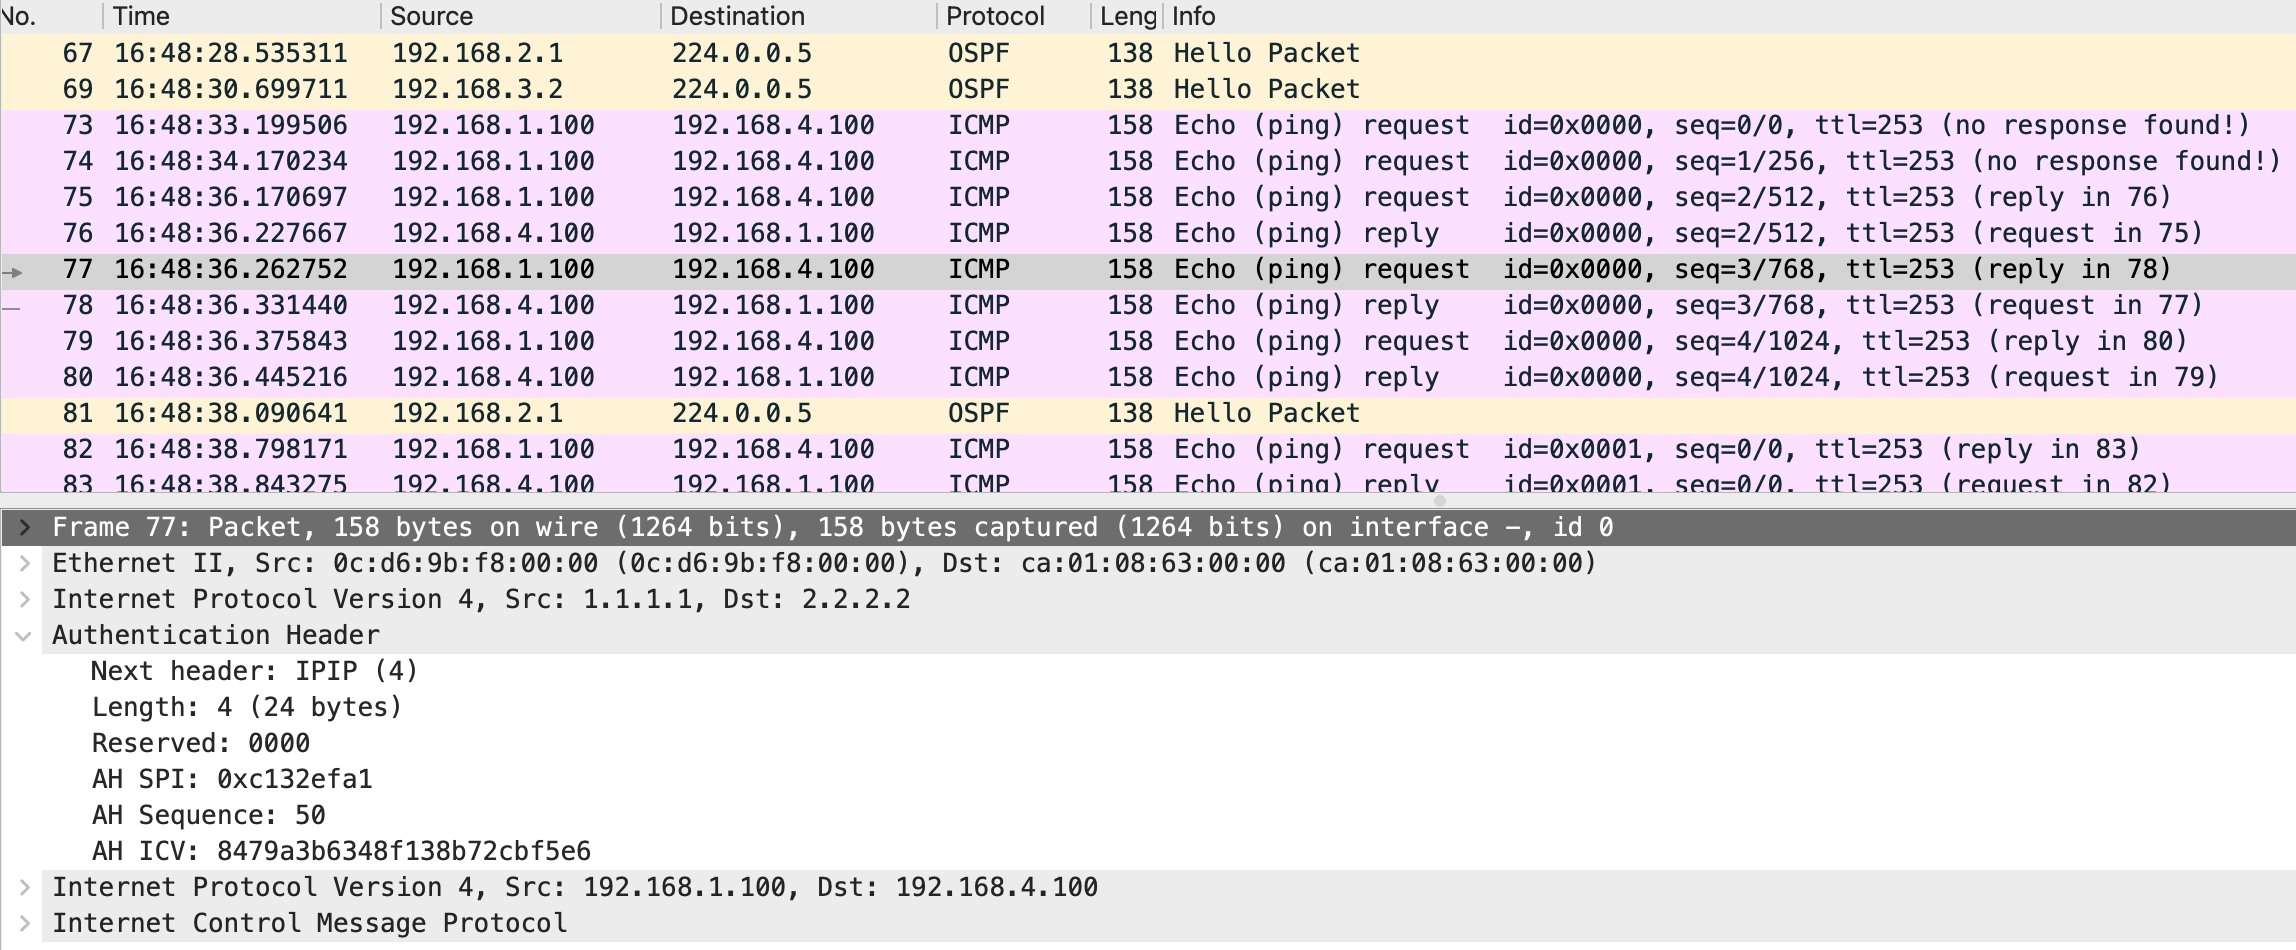
\includegraphics[width=0.95\linewidth]{../Images/1.png}
    \caption{AH protecting ICMP traffic between PC1 and PC2}
    \label{fig:ah_icmp}
\end{figure}

\subsection{OSPF Traffic Analysis}

OSPF traffic exchanged through the tunnel was also analyzed.

Figure~\ref{fig:ospf_plain} shows a normal OSPF Hello packet before IPSec protection. The packet includes the Router ID, Area ID, Hello Interval, Dead Interval, and neighbor information required for adjacency establishment.

\begin{figure}[H]
    \centering
    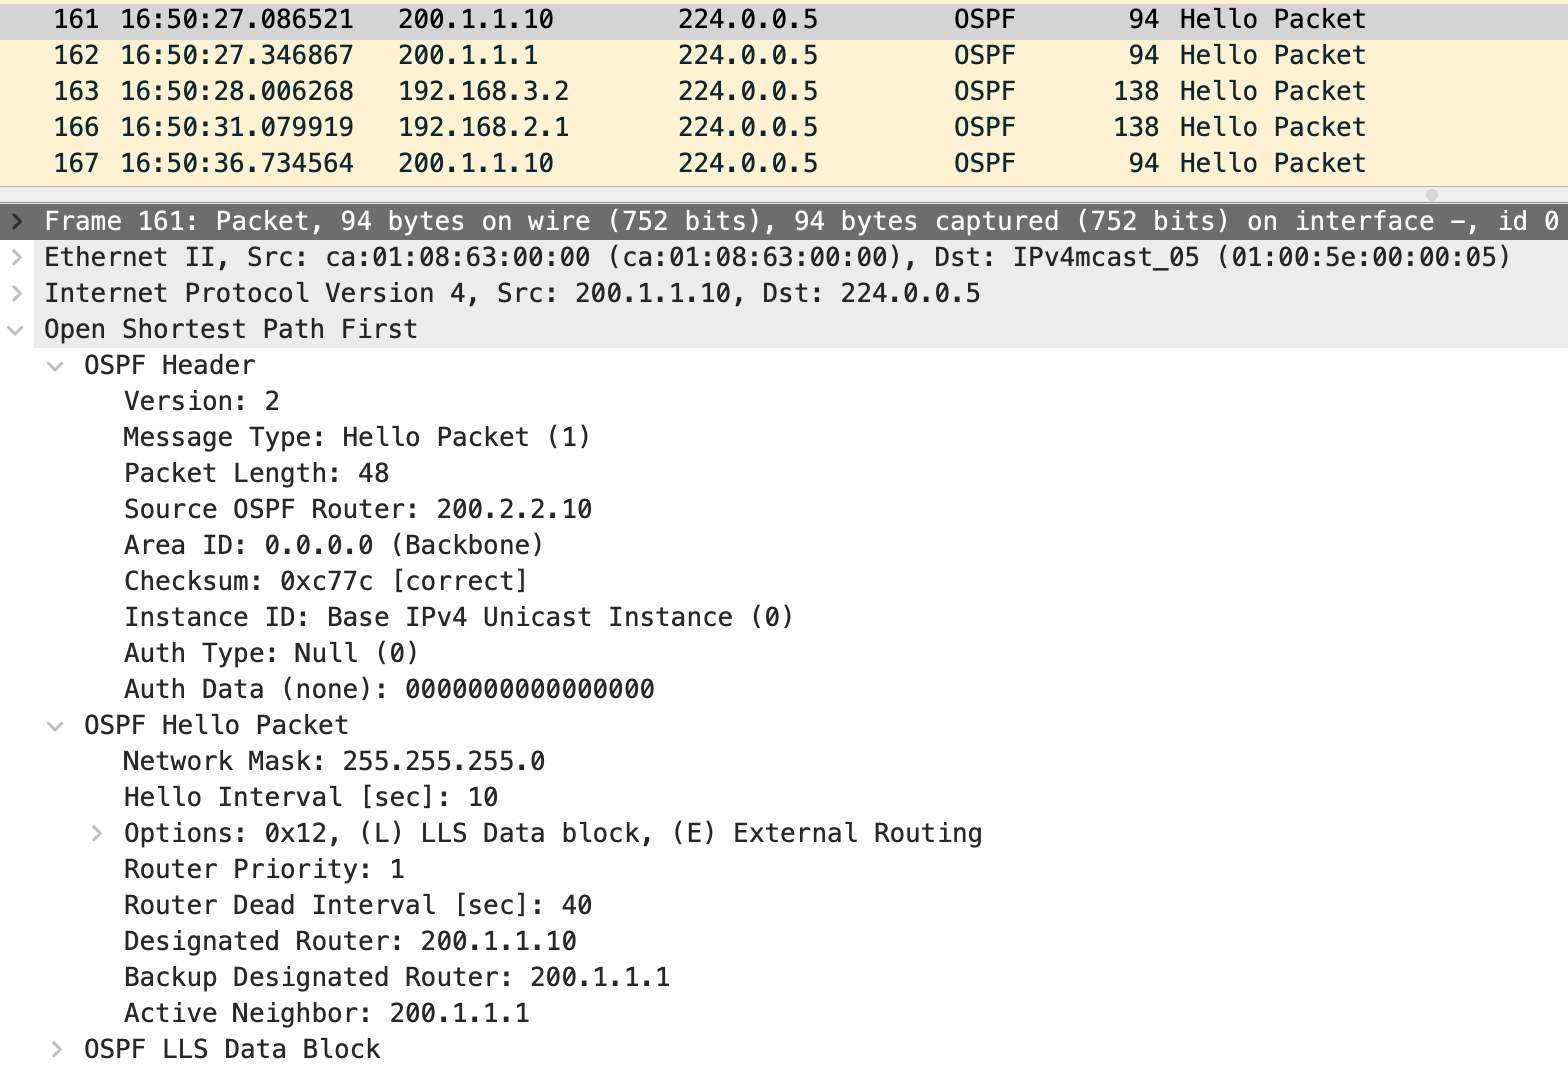
\includegraphics[width=0.95\linewidth]{../Images/2.png}
    \caption{OSPF Hello packet without IPSec protection}
    \label{fig:ospf_plain}
\end{figure}

Figure~\ref{fig:ospf_ah} shows the same OSPF traffic protected using AH. The Authentication Header appears before the OSPF packet, proving that the packet integrity and authentication are protected. However, the OSPF payload itself remains visible because AH does not provide confidentiality.

\begin{figure}[H]
    \centering
    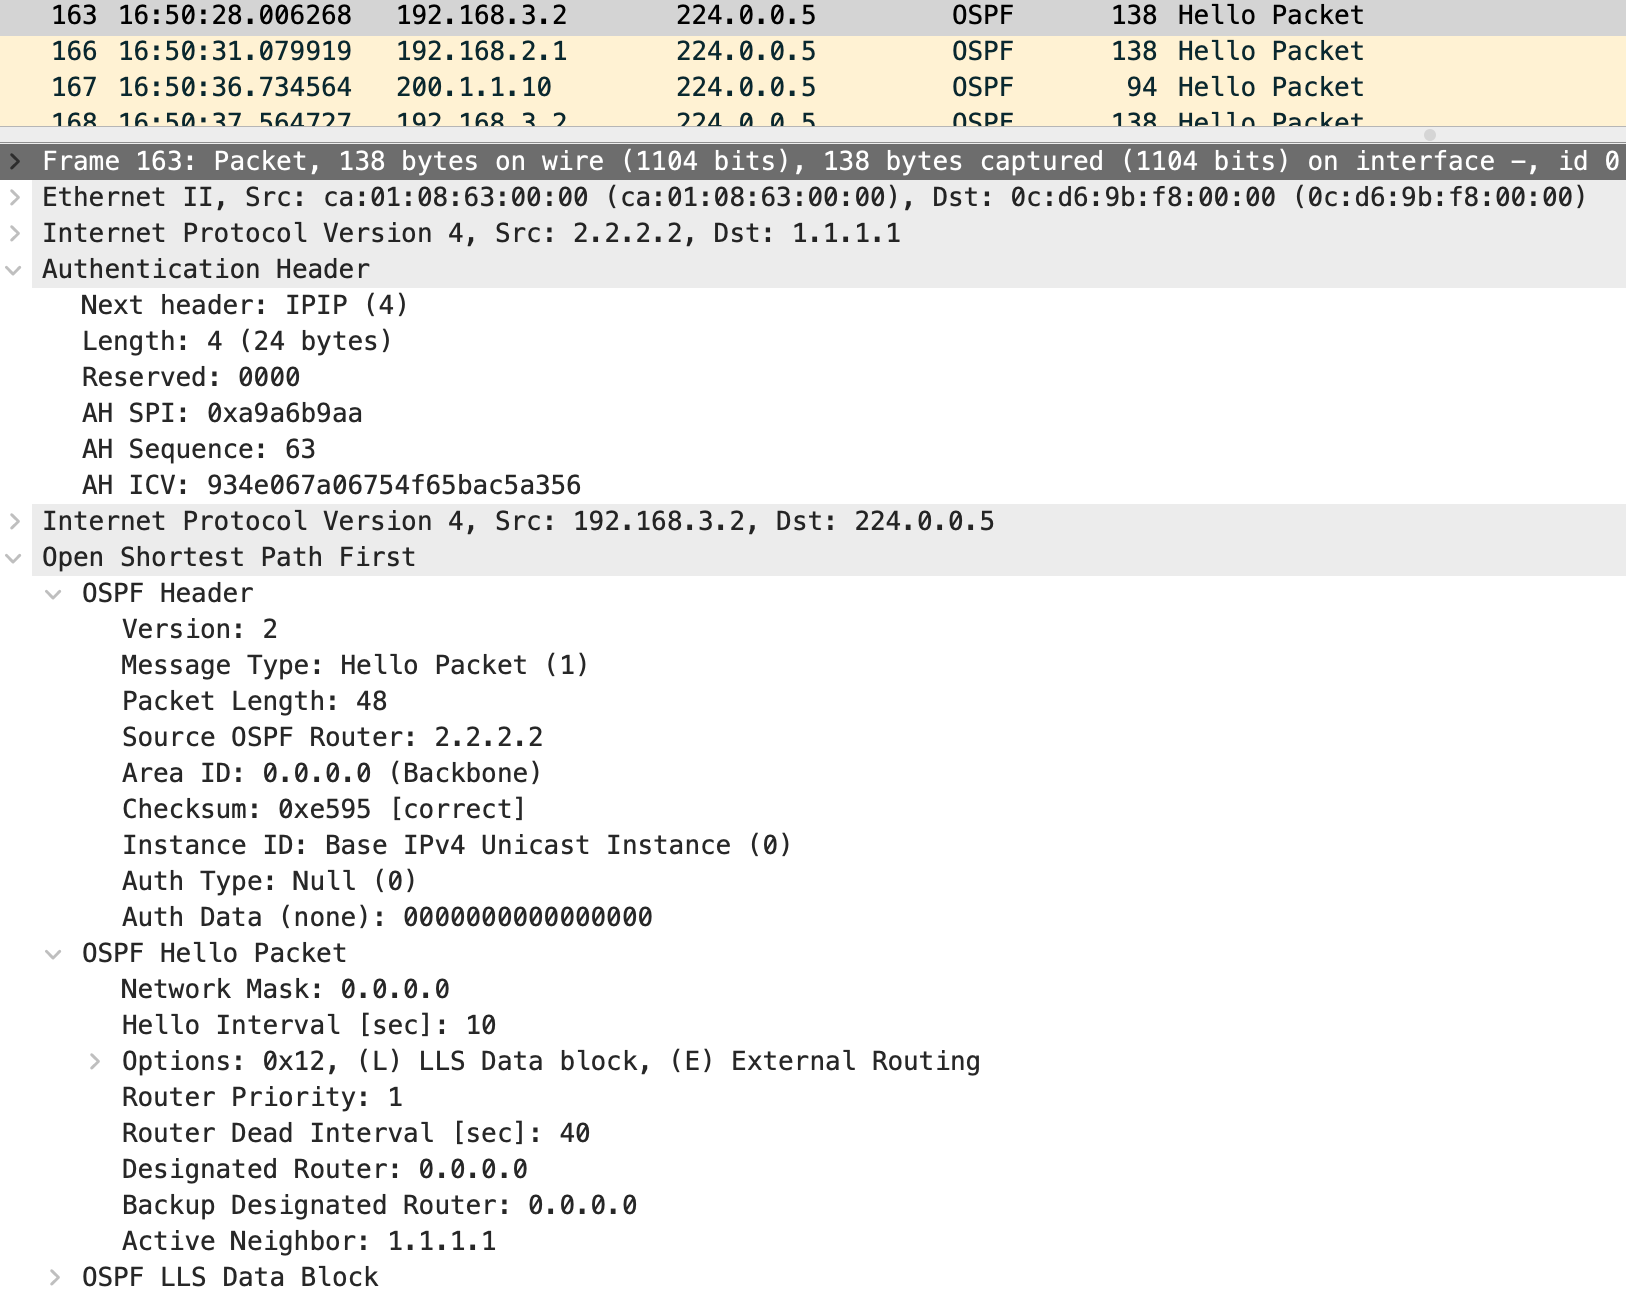
\includegraphics[width=0.95\linewidth]{../Images/3.png}
    \caption{OSPF Hello packet protected with AH}
    \label{fig:ospf_ah}
\end{figure}

\subsection{IKEv1 and ISAKMP Negotiation}

The IPSec Security Associations were cleared using the command:

\begin{verbatim}
clear crypto session
\end{verbatim}

This operation forced the routers to delete the existing IPSec tunnel and establish a new one. During this process, Wireshark captured the exchanged ISAKMP packets.

\subsubsection{ISAKMP Informational Messages}

Before re-establishing the tunnel, ISAKMP Informational messages were exchanged between peers. These messages are used to maintain or delete Security Associations.

Figure~\ref{fig:isakmp_info} shows an Informational exchange containing encrypted data.

\begin{figure}[H]
    \centering
    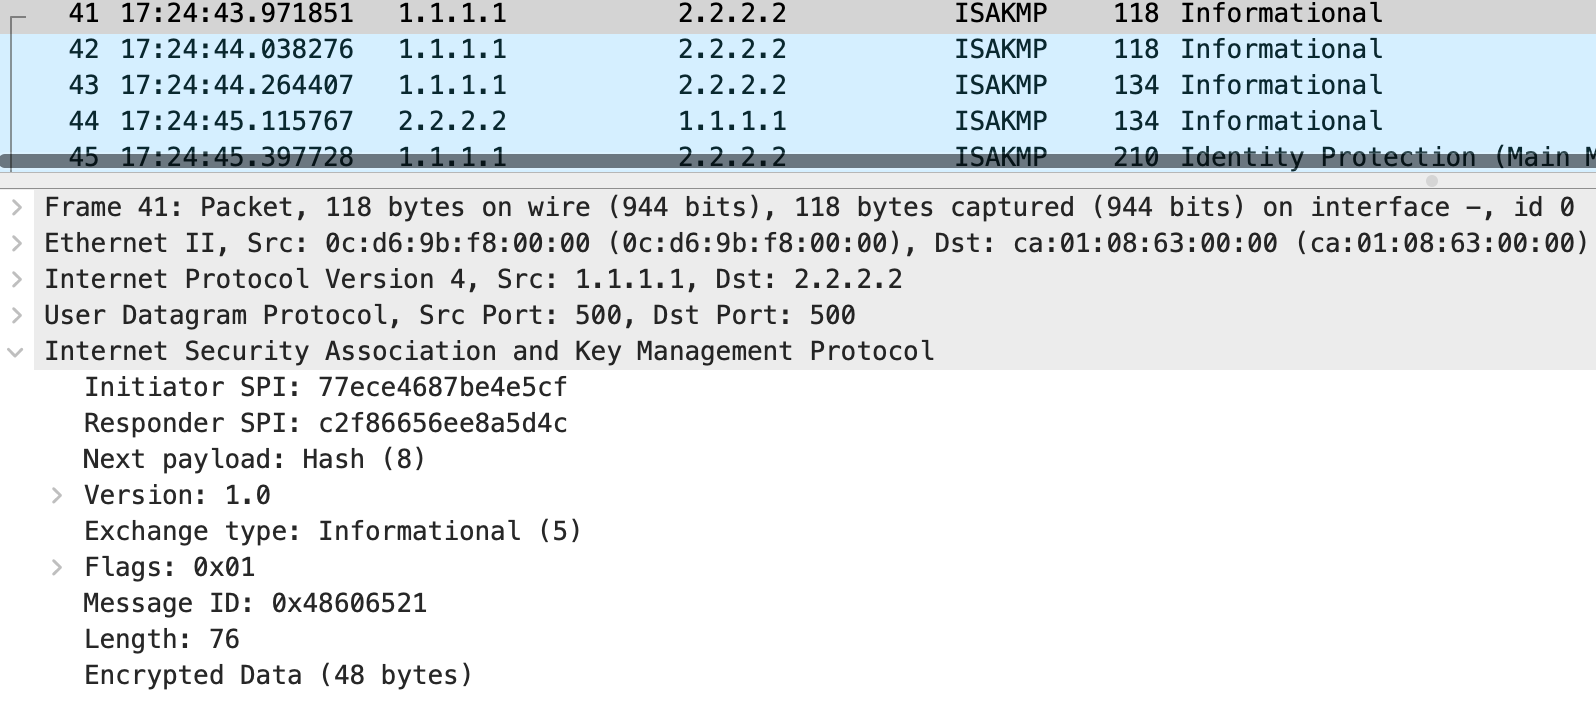
\includegraphics[width=0.95\linewidth]{../Images/4.png}
    \caption{ISAKMP Informational message}
    \label{fig:isakmp_info}
\end{figure}

\subsubsection{IKE Phase 1 -- Main Mode}

IKE Phase 1 establishes the ISAKMP Security Association used to securely negotiate IPSec parameters.

Figure~\ref{fig:mainmode_sa} shows the initial Main Mode exchange. The Security Association payload contains the proposed cryptographic algorithms and authentication methods supported by the initiator.

\begin{figure}[H]
    \centering
    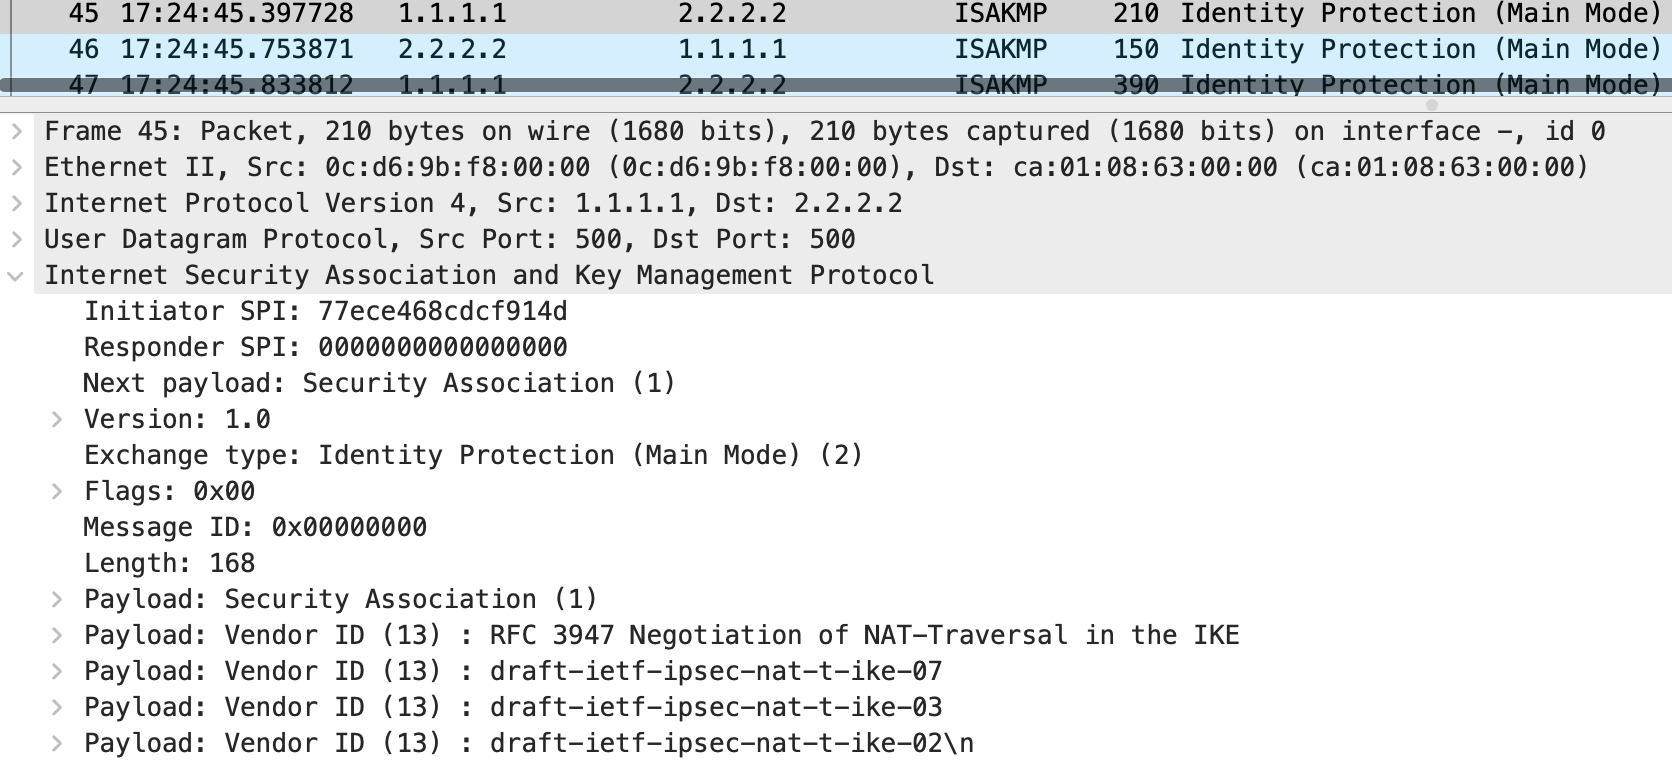
\includegraphics[width=0.95\linewidth]{../Images/5.png}
    \caption{IKEv1 Main Mode Security Association negotiation}
    \label{fig:mainmode_sa}
\end{figure}

Figure~\ref{fig:dh_exchange} shows the Diffie-Hellman exchange phase. The Key Exchange payload carries the public Diffie-Hellman values required to generate the shared secret key between both peers. The Nonce payload adds randomness to the generated keys, increasing security.

The Key Exchange payload is therefore responsible for securely generating a common secret without transmitting the secret itself over the network.

\begin{figure}[H]
    \centering
    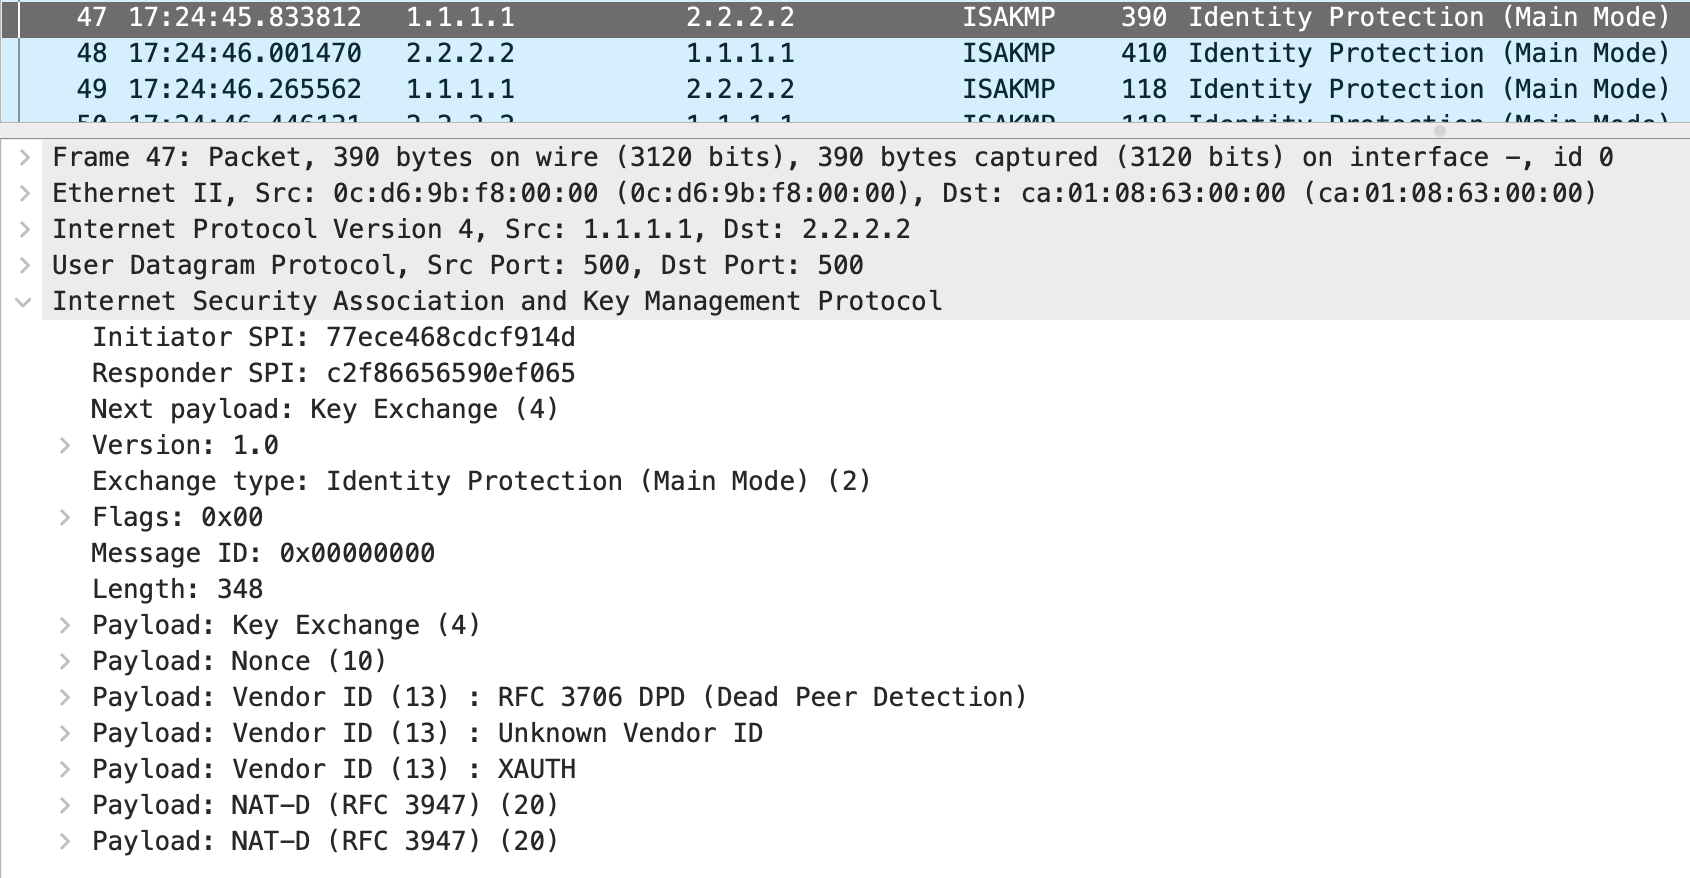
\includegraphics[width=0.95\linewidth]{../Images/6.png}
    \caption{Diffie-Hellman Key Exchange during IKE Phase 1}
    \label{fig:dh_exchange}
\end{figure}

The Nonce payload (also visible in Figure~\ref{fig:dh_exchange}) contributes a 
fresh random value to every exchange. Combined with the Diffie-Hellman output, it 
ensures that even if the same DH parameters were reused across sessions, the 
derived keying material would differ --- protecting against key reuse and replay 
attacks.

Figure~\ref{fig:identity} shows the final Main Mode exchanges where identity information and authentication data are transmitted in encrypted form. At this stage, the ISAKMP SA has already been established.

\begin{figure}[H]
    \centering
    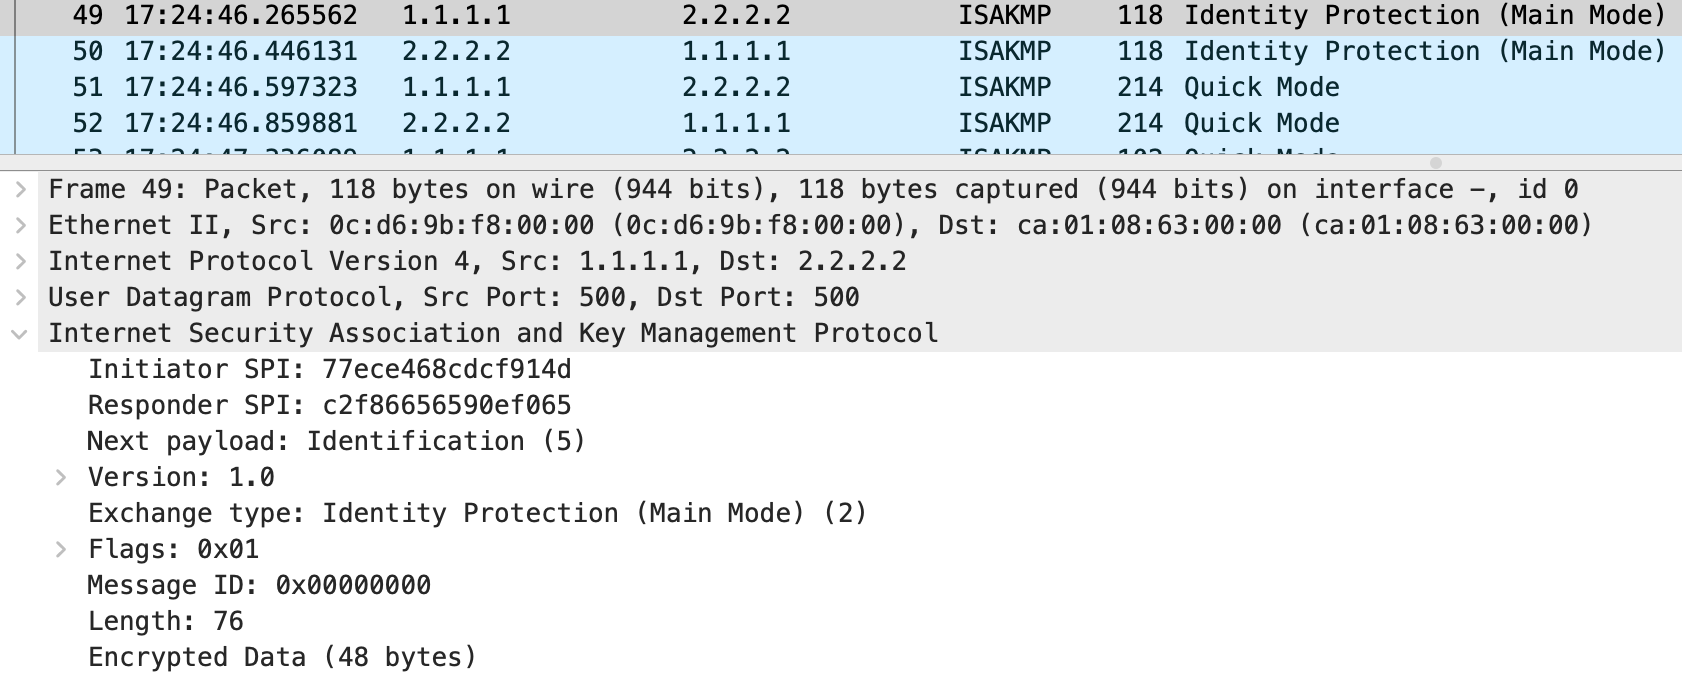
\includegraphics[width=0.95\linewidth]{../Images/7.png}
    \caption{Identity protection during IKE Phase 1}
    \label{fig:identity}
\end{figure}

\subsubsection{IKE Phase 2 -- Quick Mode}

IKE Phase 2 negotiates the IPSec Security Associations used to protect data traffic.

Figure~\ref{fig:quickmode} shows the Quick Mode exchange responsible for negotiating IPSec parameters such as AH/ESP protocols, encryption algorithms, integrity algorithms, and Security Associations.

\begin{figure}[H]
    \centering
    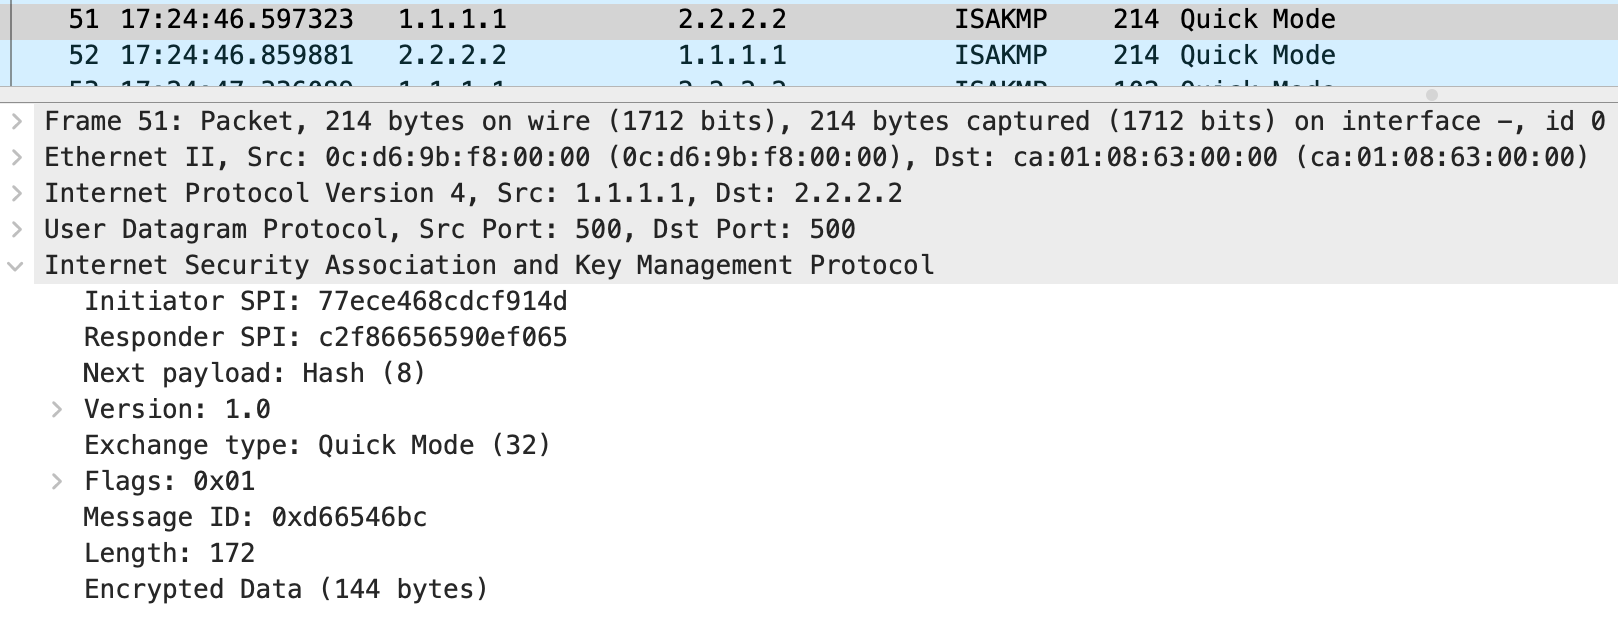
\includegraphics[width=0.95\linewidth]{../Images/8.png}
    \caption{IKE Phase 2 Quick Mode negotiation}
    \label{fig:quickmode}
\end{figure}

The router outputs confirmed the successful establishment of the tunnel. The ISAKMP state reached \texttt{QM\_IDLE}, indicating that Phase 1 and Phase 2 negotiations completed successfully.

\begin{verbatim}
Router#show crypto isakmp sa

dst             src             state          conn-id status
1.1.1.1         2.2.2.2         QM_IDLE           1002 ACTIVE
2.2.2.2         1.1.1.1         QM_IDLE           1003 ACTIVE
\end{verbatim}

The IPSec Security Associations were also verified using:

\begin{verbatim}
show crypto ipsec sa
\end{verbatim}

The output confirmed active inbound and outbound AH Security Associations.

\subsection{Negotiation Failure Analysis}

Different cryptographic parameters were intentionally configured between peers in order to analyze negotiation failures.

Figure~\ref{fig:negotiation_failure} shows repeated Main Mode and Quick Mode negotiations. Since the peers could not agree on compatible IPSec parameters, the Security Associations were not successfully established.

As a result, ICMP communication failed and no encrypted traffic was exchanged through the tunnel.

\begin{figure}[H]
    \centering
    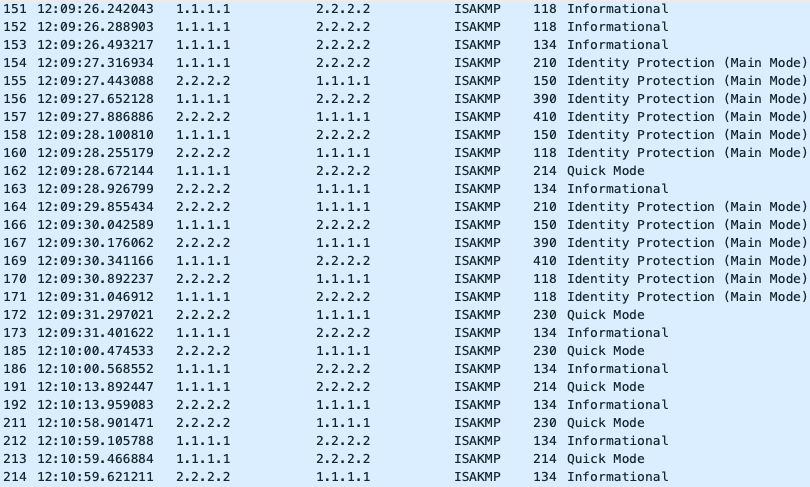
\includegraphics[width=0.95\linewidth]{../Images/10.png}
    \caption{Failed IPSec negotiation due to parameter mismatch}
    \label{fig:negotiation_failure}
\end{figure}

To trigger a negotiation failure, the IPSec protocol on R2 was changed from AH 
to ESP while R1 retained the AH configuration, creating an incompatible 
transform set. The resulting repeated Main Mode and Quick Mode exchanges are 
shown in Figure~\ref{fig:negotiation_failure}.

\subsection{ESP Tunnel Operation}

The transform set was later changed to ESP using the command:

\begin{verbatim}
crypto ipsec transform-set myTSet esp-aes esp-sha-hmac
\end{verbatim}

ESP provides confidentiality in addition to authentication and integrity.

Figure~\ref{fig:esp_packet} shows an ESP-protected packet. Unlike AH, only the ESP header remains visible, while the original payload is encrypted and cannot be inspected in Wireshark.

\begin{figure}[H]
    \centering
    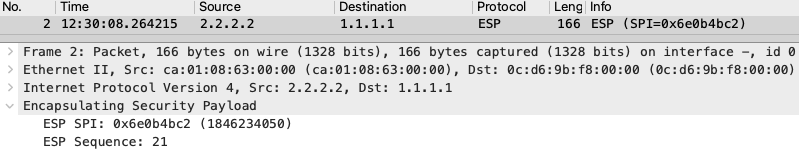
\includegraphics[width=0.95\linewidth]{../Images/11.png}
    \caption{ESP protected packet}
    \label{fig:esp_packet}
\end{figure}

Figure~\ref{fig:esp_ospf} shows ESP packets exchanged together with OSPF Hello packets during tunnel operation.

\begin{figure}[H]
    \centering
    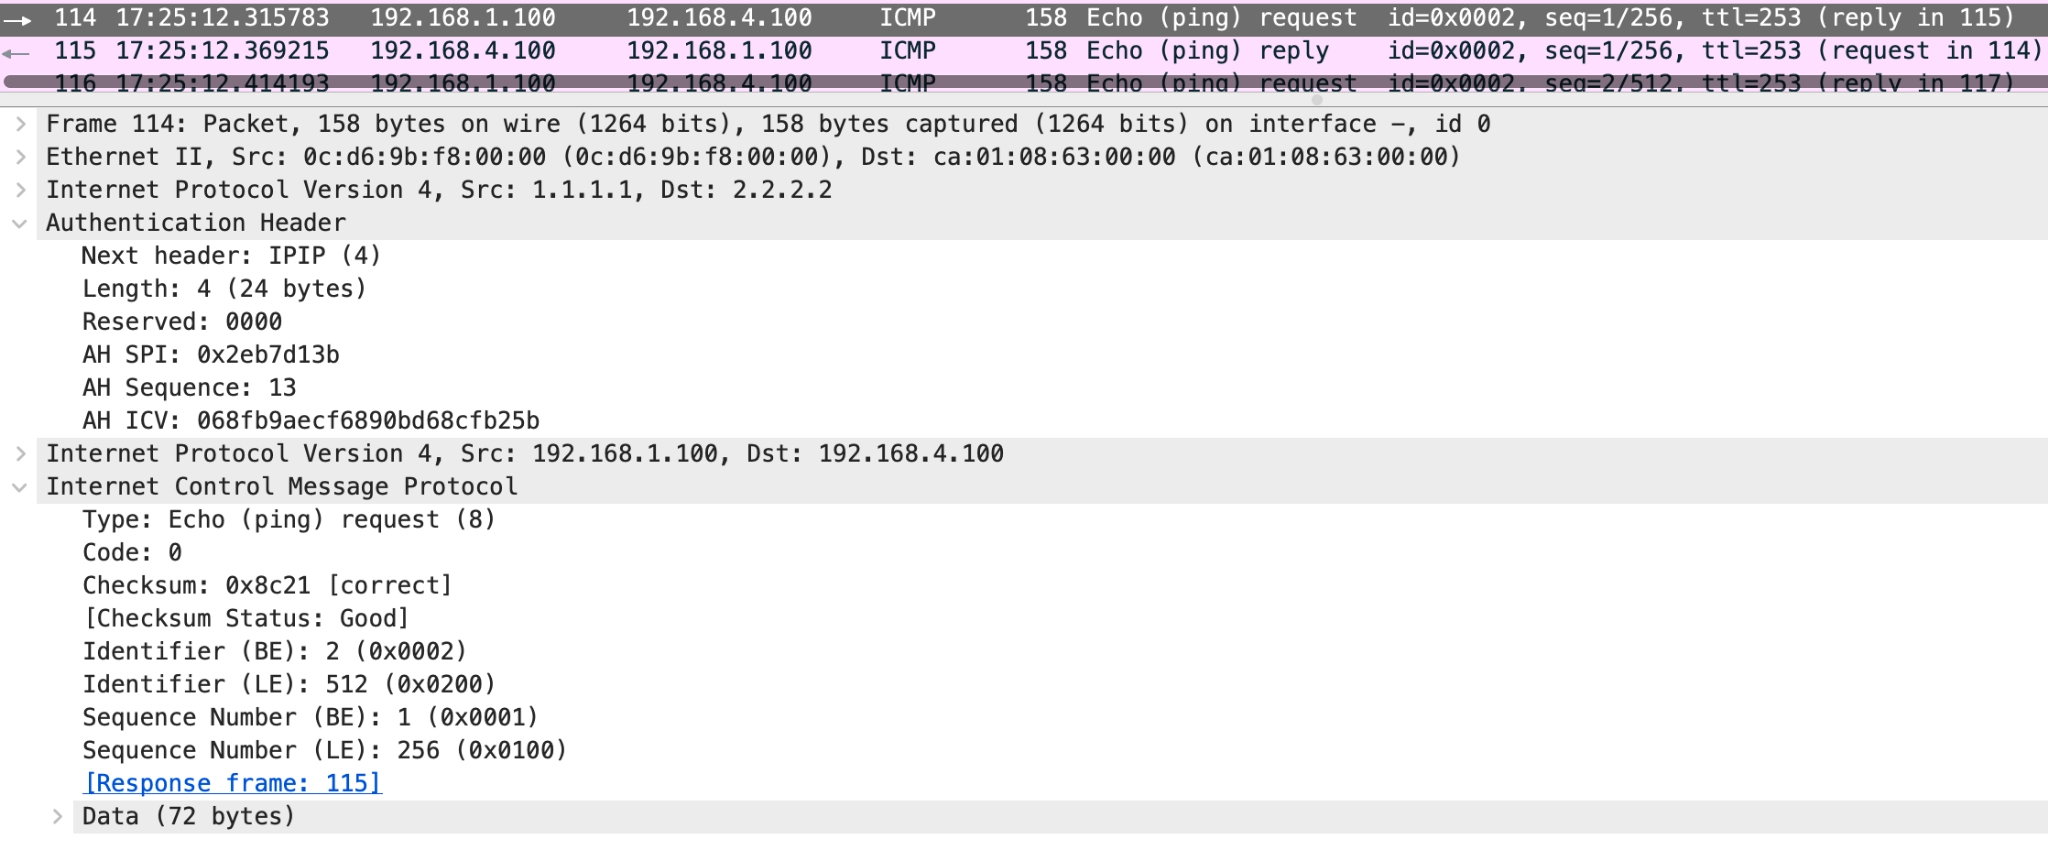
\includegraphics[width=0.95\linewidth]{../Images/9.png}
    \caption{ESP traffic and OSPF exchanges}
    \label{fig:esp_ospf}
\end{figure}

Compared to AH, ESP provides confidentiality by encrypting the payload, while AH only guarantees integrity and authentication. In AH mode, the original payload remains visible in Wireshark, whereas in ESP mode only the ESP header can be inspected and the payload contents remain encrypted.
\subsection{Firewall Requirements for IPSec}

In order for an IPSec tunnel to be successfully established through a firewall, the firewall must allow the protocols and ports used by IKE and IPSec.

The following traffic must be permitted:

\begin{itemize}
    \item UDP port 500 (ISAKMP/IKE)
    \item ESP protocol (IP protocol 50)
    \item AH protocol (IP protocol 51), when AH is used
\end{itemize}

If NAT traversal is used, UDP port 4500 must also be allowed.

Blocking any of these protocols prevents successful establishment of the IPSec tunnel.


\newpage

\section{IKEv1 with Digital Signatures}

\subsection{Introduction}

This section describes the configuration and analysis of IPSec VPN using IKEv1 with digital certificates (PKI-based authentication using SCEP). 
The objective is to replace pre-shared keys with RSA signatures issued by a Certification Authority (CA).

\subsection{Topology Overview}

RA operates as the Certification Authority (CA) and NTP server. 
R1 and R2 establish an IPSec tunnel authenticated using RSA signatures and certificates obtained through SCEP enrollment.

\subsection{PKI Installation Verification}

The Certification Authority (CA) and router certificates were verified using IOS show commands.

\subsubsection{CA Configuration and Certificate (RA)}

The CA is configured on router RA and operates in automatic enrollment mode.

\begin{verbatim}
RA#show crypto pki server
Certificate Server myCA:
    Status: enabled
    State: enabled
    Server's configuration is locked  (enter "shut" to unlock it)
    Issuer name: cn=saarCA
    CA cert fingerprint: 46CB9C10 CC370311 8CFCB545 E4DD2F58 
    Granting mode is: auto
    Last certificate issued serial number (hex): 1
    CA certificate expiration timer: 16:17:23 UTC May 14 2029
    CRL NextUpdate timer: 22:17:23 UTC May 15 2026
    Current primary storage dir: nvram:
    Database Level: Minimum - no cert data written to storage
\end{verbatim}

The CA certificate installed on RA confirms that RA is acting as a trusted root authority:

\begin{verbatim}
RA#show crypto ca certificate
CA Certificate
  Status: Available
  Certificate Serial Number (hex): 01
  Certificate Usage: Signature
  Issuer: 
    cn=saarCA
  Subject: 
    cn=saarCA
  Validity Date: 
    start date: 16:17:23 UTC May 15 2026
    end   date: 16:17:23 UTC May 14 2029
  Associated Trustpoints: myCA 
  Storage: nvram:saarCA#1CA.cer
\end{verbatim}

The detailed certificate view confirms RSA key usage and X.509 extensions:

\begin{verbatim}
RA#show crypto ca certificate verbose
CA Certificate
  Status: Available
  Version: 3
  Certificate Serial Number (hex): 01
  Certificate Usage: Signature
  Issuer: 
    cn=saarCA
  Subject: 
    cn=saarCA
  Validity Date: 
    start date: 16:17:23 UTC May 15 2026
    end   date: 16:17:23 UTC May 14 2029
  Subject Key Info:
    Public Key Algorithm: rsaEncryption
    RSA Public Key: (1024 bit)
  Signature Algorithm: MD5 with RSA Encryption
  Fingerprint MD5: 46CB9C10 CC370311 8CFCB545 E4DD2F58 
  Fingerprint SHA1: 0B6BF47E F0932FC1 54A33FA8 4C1F48D1 80083958 
  X509v3 extensions:
    X509v3 Key Usage: 86000000
      Digital Signature
      Key Cert Sign
      CRL Signature
    X509v3 Subject Key ID: 42BD5391 0D07D957 6CC26630 AABA09E4 A93162E2 
    X509v3 Basic Constraints:
        CA: TRUE
    X509v3 Authority Key ID: 42BD5391 0D07D957 6CC26630 AABA09E4 A93162E2 
    Authority Info Access:
  Associated Trustpoints: myCA 
  Storage: nvram:saarCA#1CA.cer
\end{verbatim}

\subsubsection{Router Certificates (R1)}

R1 successfully enrolled with the CA and received both the CA certificate and its own identity certificate:

\begin{verbatim}
R1#show crypto pki certificates
Certificate
  Status: Available
  Certificate Serial Number (hex): 03
  Certificate Usage: General Purpose
  Issuer: 
    cn=saarCA
  Subject:
    Name: R1
    Serial Number: 9SO8DYF8WAKSOLHEG3ZVL
    hostname=R1+serialNumber=9SO8DYF8WAKSOLHEG3ZVL
  Validity Date: 
    start date: 16:33:16 UTC May 15 2026
    end   date: 16:33:16 UTC May 15 2027
  Associated Trustpoints: myTrustpoint 
\end{verbatim}

The CA certificate is also stored locally to validate the trust chain:

\begin{verbatim}
CA Certificate
  Status: Available
  Certificate Serial Number (hex): 01
  Certificate Usage: Signature
  Issuer: 
    cn=saarCA
  Subject: 
    cn=saarCA
  Validity Date: 
    start date: 16:17:23 UTC May 15 2026
    end   date: 16:17:23 UTC May 14 2029
  Associated Trustpoints: myTrustpoint
\end{verbatim}

\subsubsection{RSA Public Keys (R1 and R2)}

The RSA public keys generated on R1 and R2 are extracted using the following IOS command:

\begin{verbatim}
show crypto key mypub rsa
\end{verbatim}

\textbf{R2 RSA Public Key:}

\begin{verbatim}
R2#show crypto key mypub rsa
% Key pair was generated at: 16:32:05 UTC May 15 2026
Key name: R2
Key type: RSA KEYS
 Storage Device: private-config
 Usage: General Purpose Key
 Key is not exportable.
 Key Data:
  30819F30 0D06092A 864886F7 0D010101 05000381 8D003081 89028181 00C337FE 
  B0DAEE4D 444B0AF7 A19A73B3 2D2FCD5E 27E09095 3017E393 2F27F7AA 581894E6 
  5E7F50B3 0454ACF2 FD1E8E24 F91125DD 6D611D93 611D70AD 36C59F6F EAEE003C 
  7704B6DB 41D9A165 27252864 17170DA2 F38A68D4 46C91133 36DBCBC5 B09AD90E 
  0F05531B F7ABB4A5 0B954C0F 389C2195 3DE377FF 7FE63FB3 B02DF189 35020301 
  0001
% Key pair was generated at: 16:57:46 UTC May 16 2026
Key name: R2.server
Key type: RSA KEYS
Temporary key
 Usage: Encryption Key
 Key is not exportable.
 Key Data:
  307C300D 06092A86 4886F70D 01010105 00036B00 30680261 00A38B5F B33F29E4 
  E5E30AFB 512084C9 0A89E015 BCA1569A C10C686B B79BD8EC C3C25CAD 6EE74C8F 
  C891E5FF 1B042503 710EC940 65712523 377F2776 77CDC4C0 D7D61754 57C88063 
  19BF191B F48130CC 327EF733 1F877D95 5CB74450 AEEF7E99 45020301 0001
\end{verbatim}

\textbf{R1 RSA Public Key:}

\begin{verbatim}
R1#show crypto key mypub rsa
% Key pair was generated at: 16:31:43 UTC May 15 2026
Key name: R1
Key type: RSA KEYS
 Storage Device: private-config
 Usage: General Purpose Key
 Key is not exportable.
 Key Data:
  30819F30 0D06092A 864886F7 0D010101 05000381 8D003081 89028181 00DF87BB 
  11BD33EE C4E9DF4A C2FF2CCB 2ECCEFF9 713AAA45 633ADE4A C188109E 88680D67 
  FB0A2F20 67257007 79DB3616 75D5459A 4898DE69 E74E80BA 77C993E8 A4B70D41 
  00D1D2FB E37BF0E3 89C8BEEE 9830712E 8A4C13DC E30C5C72 D72FEDF2 A221F6DB 
  9A1A1B8F 9A69BC61 3700CA1B B66DB044 72F24609 E0C1FE8D 24D1B3DA DD020301 
  0001
% Key pair was generated at: 16:57:42 UTC May 16 2026
Key name: R1.server
Key type: RSA KEYS
Temporary key
 Usage: Encryption Key
 Key is not exportable.
 Key Data:
  307C300D 06092A86 4886F70D 01010105 00036B00 30680261 0095CC14 73EE9BA8 
  1B0A40A6 E3EE90C1 BC2FAADF 2D532270 160D9039 C19C40CA 6A4E54B5 BAB8892C 
  D266AE9A 53210F58 876755F6 381C44B6 5D71F57F 35705BC5 3E8D9746 61833A6A 
  DB5E740B 8A22A486 83EE7AFA ACAB3798 27D03FC2 7C6EA875 FD020301 0001
\end{verbatim}

Both routers generate 1024-bit RSA key pairs used for digital signature authentication during IKEv1 Phase 1.

\subsection{SCEP Enrollment Analysis}

SCEP (Simple Certificate Enrollment Protocol) is used to automate certificate distribution between routers and the CA using HTTP.

The enrollment process consists of:

\begin{itemize}
\item \texttt{CA certificate request}
\item \texttt{CA certificate response}
\item \texttt{Router certificate request}
\item \texttt{Router certificate issuance}
\end{itemize}

\subsubsection{CA Certificate Retrieval}

Initially, R1 requests the CA certificate using the SCEP \texttt{GetCACert} operation over HTTP.

\begin{figure}[H]
\centering
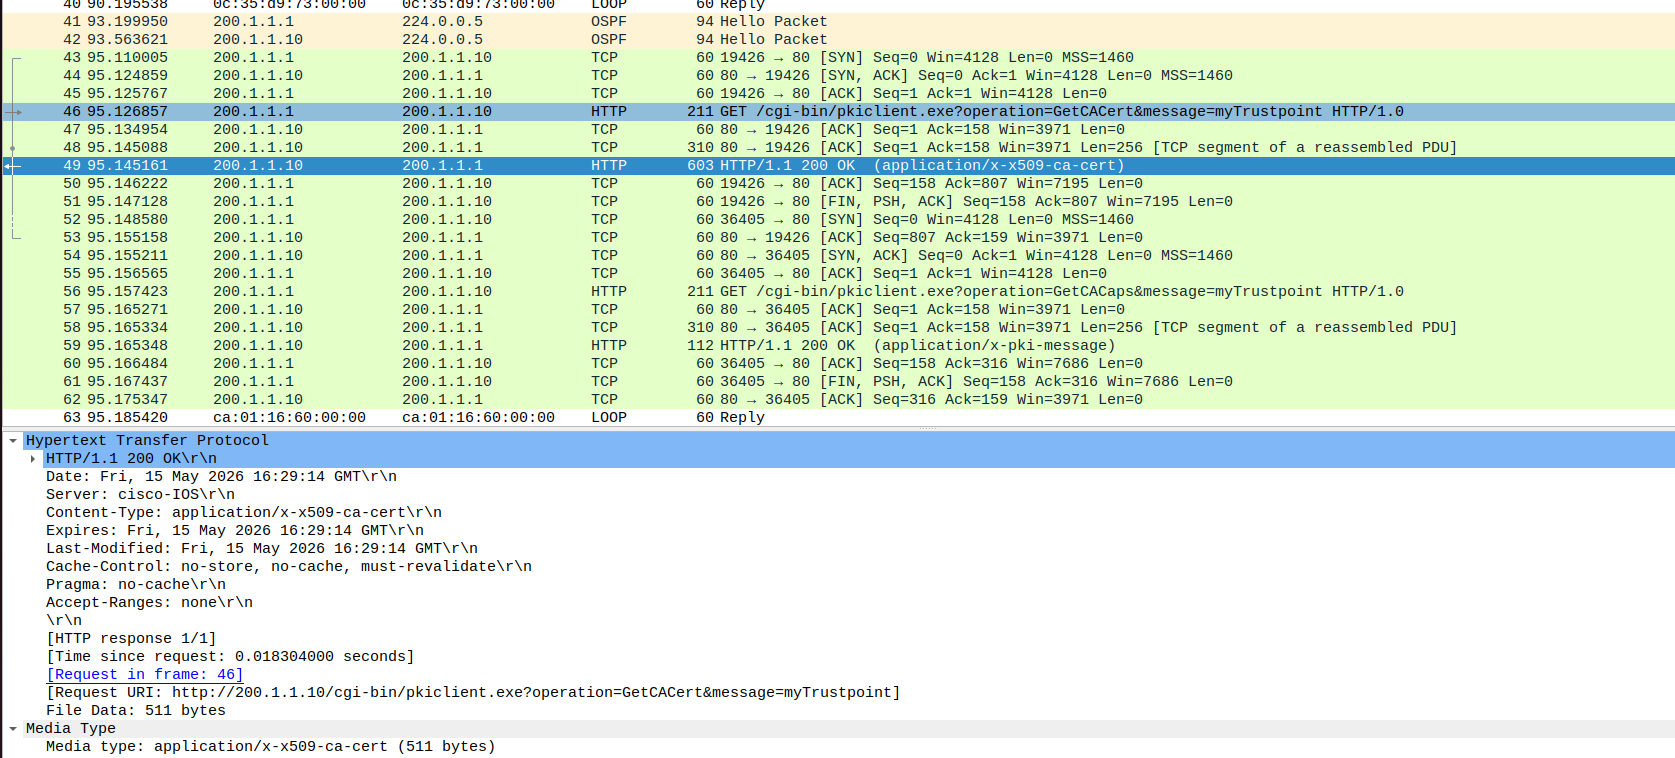
\includegraphics[width=\linewidth]{../Images/R1-RA_cerificate_exchange.png}
\caption{SCEP GetCACert request and CA certificate response}
\label{fig:getcacert}
\end{figure}

The CA replies with an HTTP \texttt{200 OK} message containing an X.509 CA certificate with media type \texttt{application/x-x509-ca-cert}. This certificate allows R1 to establish trust with the Certification Authority before certificate enrollment.

\subsubsection{Certificate Enrollment Request}

After establishing trust with the CA, R1 performs certificate enrollment using the SCEP \texttt{PKIOperation} request.

\begin{figure}[H]
\centering
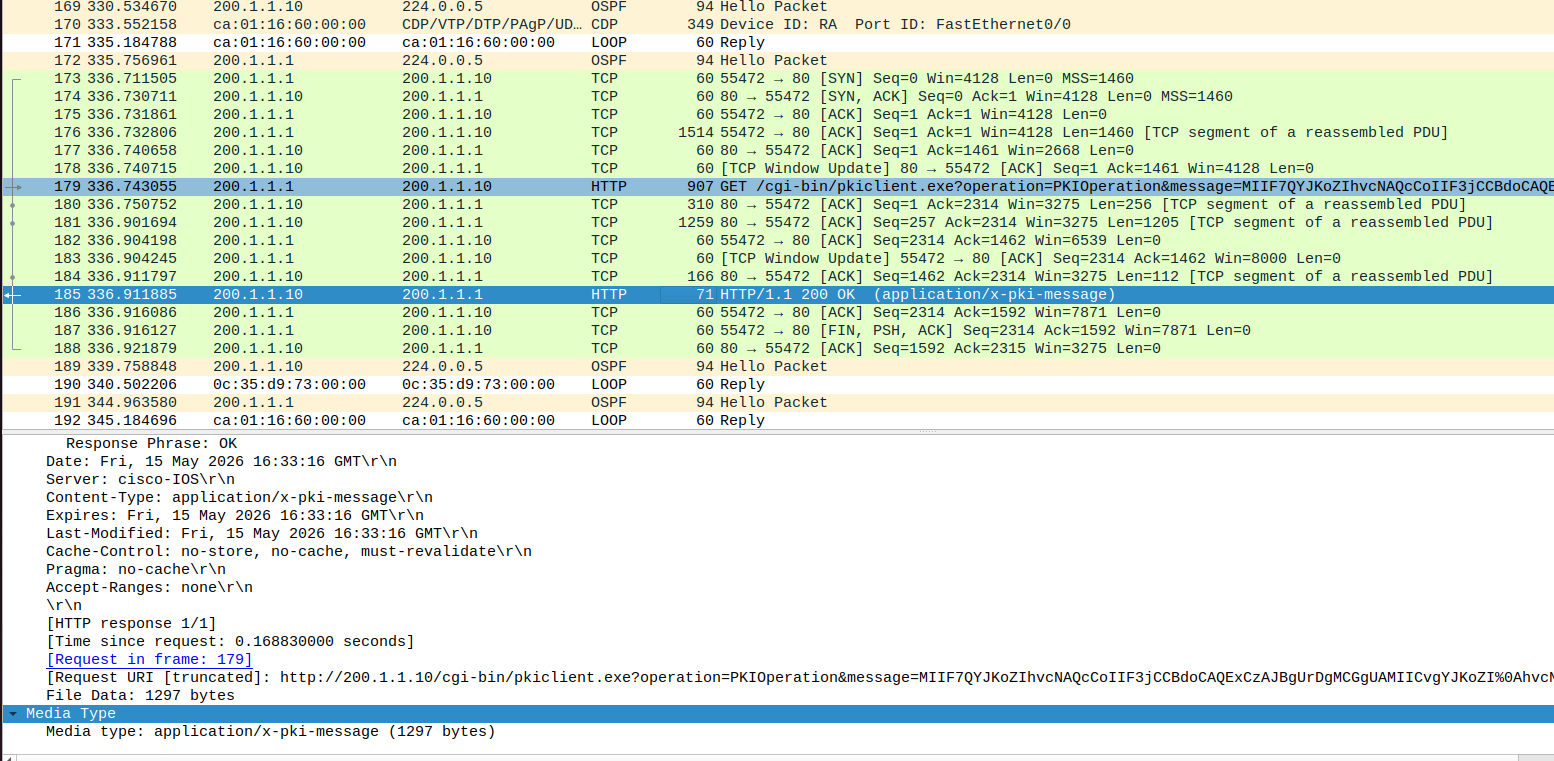
\includegraphics[width=\linewidth]{../Images/R1-RA_PKIOperation.png}
\caption{SCEP PKIOperation certificate enrollment request}
\label{fig:pkioperation}
\end{figure}

The HTTP request contains a PKCS\#10 certificate signing request (CSR) encoded in the message field. The CSR includes the router identity and its RSA public key, allowing the CA to generate a signed X.509 certificate for R1.

The captured HTTP messages show certificate exchange between R1 and the CA. The content-type field indicates certificate payload transfer (.crt).

Using Wireshark, the packet containing the issued certificate was identified by filtering HTTP traffic and locating the response message with a \texttt{Media Type} indicating a certificate object. The packet was then selected, and the certificate data was extracted by right-clicking on the relevant field and choosing \textit{Export Packet Bytes}. The file was saved with a \texttt{.crt} extension, which allows it to be decoded as an X.509 certificate.

\begin{figure}[H]
\centering
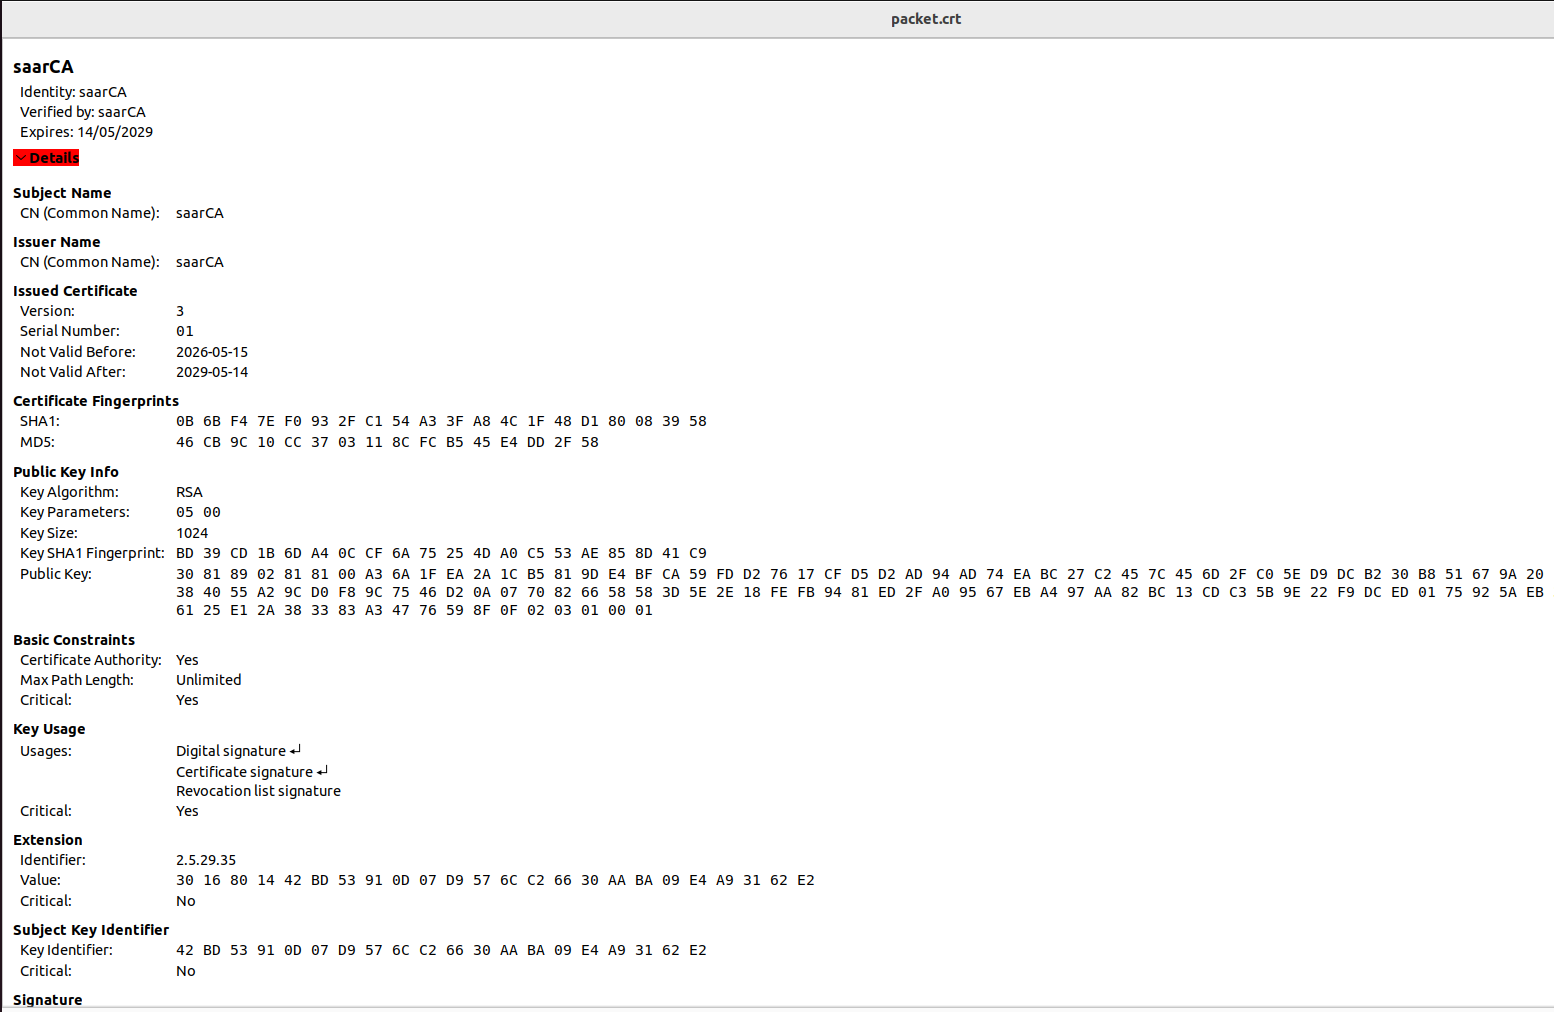
\includegraphics[width=\linewidth]{../Images/R1-RA-certificate-packet.png}
\caption{HTTP packet carrying the issued X.509 certificate (.crt file export in Wireshark)}
\label{fig:crtpacket}
\end{figure}

The exported certificate represents the CA-signed identity certificate for R1. It contains the subject information, the public key corresponding to R1, and the digital signature generated by the CA, which validates its authenticity within the PKI infrastructure.

\subsection{Encrypted ICMP Traffic Analysis}

After configuring IPSec with RSA-signature authentication, connectivity between PC1 and PC2 was successfully verified using ICMP echo requests (ping).

Traffic was captured on the public network between R1 and R2 while the ping operation was performed.

\begin{figure}[H]
\centering
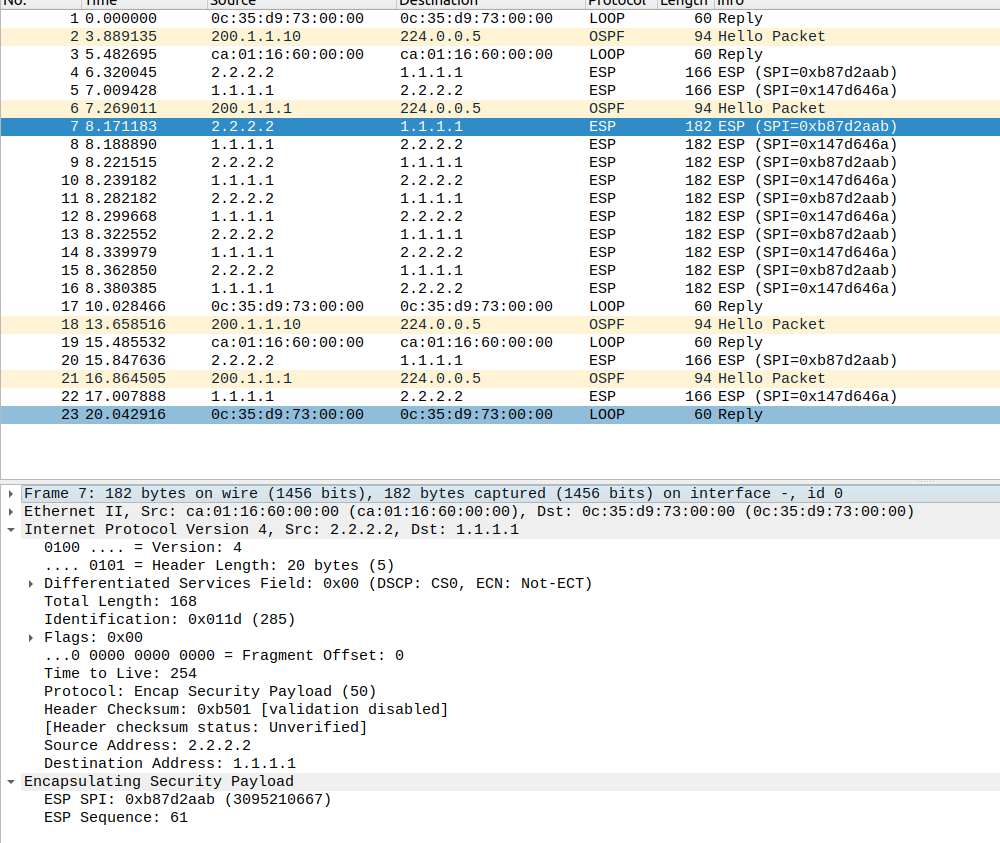
\includegraphics[width=\linewidth]{../Images/Ping_PCs_ESP.png}
\caption{Encrypted IPSec traffic observed between R1 and R2}
\label{fig:encryptedicmp}
\end{figure}

The Wireshark capture shows that the ICMP packets exchanged between PC1 and PC2 are not visible in plaintext on the public network. Instead, the packets appear encapsulated using ESP (Encapsulating Security Payload).

The ESP packets contain encrypted payload data, preventing direct inspection of the original ICMP echo request and echo reply contents. Only the external IP header remains visible, showing communication between the tunnel endpoints (R1 and R2).

This confirms that IPSec is correctly providing:
\begin{itemize}
\item \textbf{Confidentiality} through payload encryption
\item \textbf{Integrity protection} through ESP authentication
\item \textbf{Secure tunnel encapsulation} between the two sites
\end{itemize}

The observed ESP traffic corresponds to the IPSec transform-set configuration:

\begin{verbatim}
crypto ipsec transform-set myTSet esp-aes esp-sha-hmac
\end{verbatim}

AES is used for encryption while SHA-HMAC is used for integrity verification.

\subsection{ISAKMP and SA Re-establishment Analysis}

To analyze tunnel re-establishment, the IPSec Security Associations (SAs) were manually cleared using:

\begin{verbatim}
clear crypto session
\end{verbatim}

While capturing traffic on the public network, new ISAKMP exchanges were observed as the routers negotiated fresh IPSec Security Associations.

\begin{figure}[H]
\centering
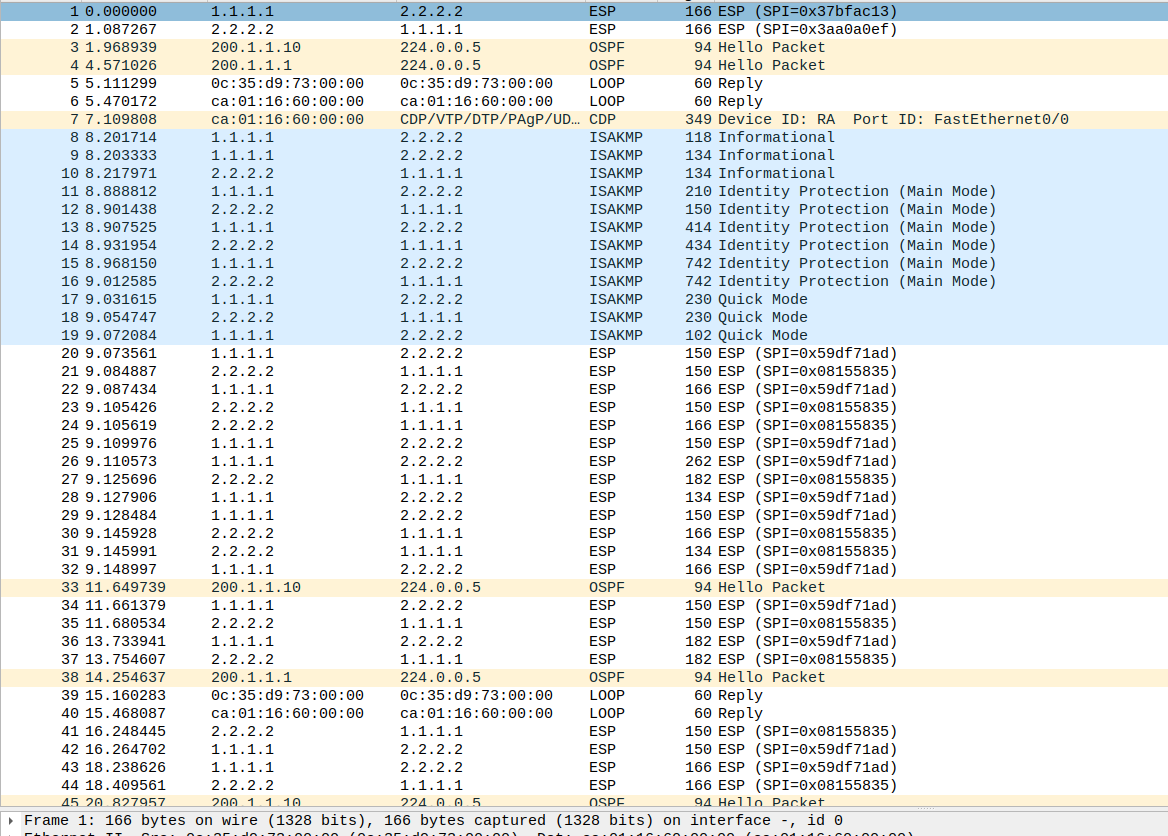
\includegraphics[width=\linewidth]{../Images/clear session msgs.png}
\caption{ISAKMP exchanges after clearing crypto sessions}
\label{fig:isakmp}
\end{figure}

After the existing SAs were deleted, R1 and R2 initiated a new IKEv1 Phase 1 negotiation using ISAKMP messages over UDP port 500.

The captured exchange shows the following operations:

\begin{itemize}
\item ISAKMP SA proposal negotiation
\item Exchange of nonces and Diffie-Hellman values
\item Certificate exchange between peers
\item RSA digital signature authentication
\item Establishment of a new ISAKMP Security Association
\item Negotiation of IPSec Phase 2 parameters
\item Creation of new IPSec SAs for ESP traffic
\end{itemize}

The certificate-based authentication process relies on the X.509 certificates previously obtained from the CA through SCEP enrollment.

During authentication, each router validates:
\begin{itemize}
\item The peer certificate authenticity
\item The CA signature
\item The RSA signature generated during IKE authentication
\end{itemize}

Successful validation allows the tunnel to be securely re-established without the use of pre-shared keys.

The re-established IPSec tunnel was confirmed by successful encrypted ICMP communication between PC1 and PC2 after the negotiation process completed.

\subsection{Peer Public Key Storage Verification}

After successful IKEv1 authentication and IPSec tunnel establishment, each router stores the public key information of the remote peer.

At R1, the public key of R2 can be viewed using:

\begin{verbatim}
show crypto key pubkey-chain rsa name R2
\end{verbatim}

The output confirms that R1 has learned and stored the RSA public key associated with R2's certificate.

\begin{verbatim}
R1#sh crypto key pubkey-chain rsa name R2
 Key name: R2 
 Subject name(X.500 DN name): hostname=R2+serialNumber=9C92ZG7WMXGLWHR7XWAK8
 Key id: 11 
 Serial number: 02
 Usage: Signature Key
 Source: Certificate
 Data:
  30819F30 0D06092A 864886F7 0D010101 05000381 8D003081 89028181 00C337FE 
  B0DAEE4D 444B0AF7 A19A73B3 2D2FCD5E 27E09095 3017E393 2F27F7AA 581894E6 
  5E7F50B3 0454ACF2 FD1E8E24 F91125DD 6D611D93 611D70AD 36C59F6F EAEE003C 
  7704B6DB 41D9A165 27252864 17170DA2 F38A68D4 46C91133 36DBCBC5 B09AD90E 
  0F05531B F7ABB4A5 0B954C0F 389C2195 3DE377FF 7FE63FB3 B02DF189 35020301 
  0001
\end{verbatim}

This public key is extracted from the X.509 certificate presented by R2 during the IKEv1 authentication process.

The stored public key allows R1 to:
\begin{itemize}
\item Verify digital signatures generated by R2
\item Validate the identity of the remote peer
\item Establish trusted IPSec communications
\end{itemize}

Similarly, R2 stores the public key of R1 after successful authentication.

The existence of the peer public key chain confirms that certificate-based authentication using RSA signatures was successfully completed and that both routers trust certificates issued by the Certification Authority.

\subsection{SCEP Messages Observed After Router Restart}

After stopping and restarting all routers, Wireshark captures were collected on the public network shortly after boot.

During startup, HTTP messages related to SCEP were again exchanged between the routers and the CA.

\begin{figure}[H]
\centering
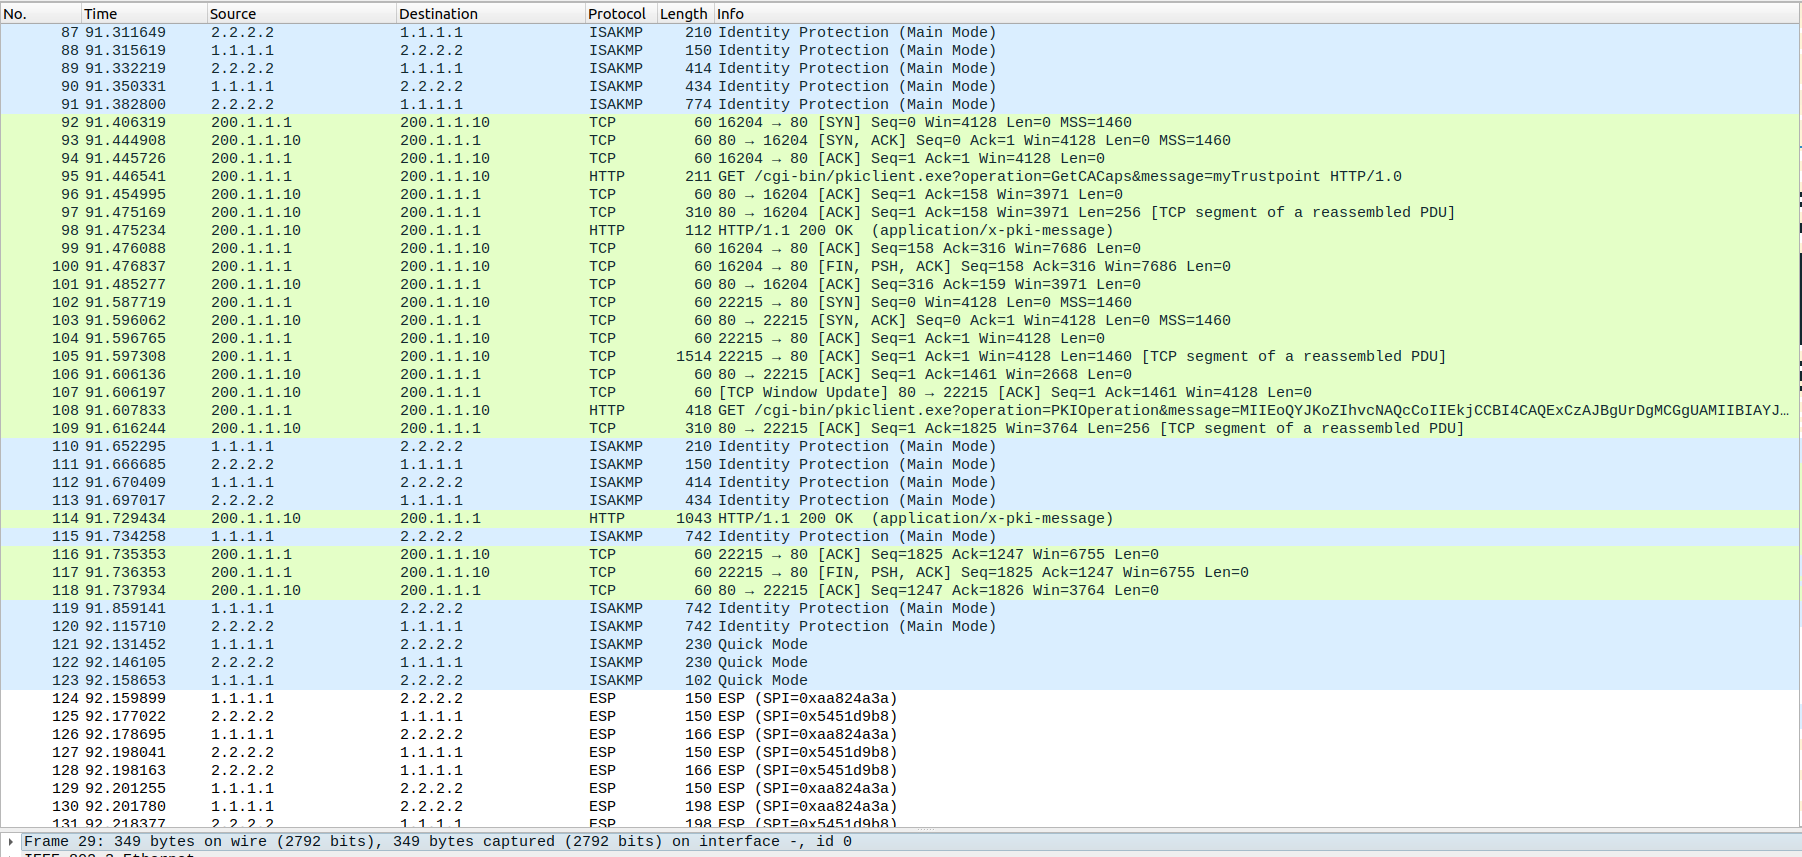
\includegraphics[width=\linewidth]{../Images/Restarted nodes screenshot.png}
\caption{SCEP-related HTTP traffic observed after router restart}
\label{fig:scep_reboot}
\end{figure}

The captured traffic includes HTTP requests and responses associated with certificate validation and certificate status retrieval operations.

These SCEP exchanges occur because the routers must re-establish trust information after reboot and verify the validity of the installed certificates before using them for IPSec authentication.

The observed messages serve several purposes:

\begin{itemize}
\item Verification that the CA is reachable
\item Retrieval or validation of CA information
\item Validation of certificate status
\item Synchronization of trust-related information
\end{itemize}

This mechanism ensures that routers do not use invalid, expired, or revoked certificates during IKEv1 authentication.

The SCEP communication therefore plays an essential role in maintaining the integrity and trustworthiness of the PKI infrastructure used for IPSec VPN authentication.

\subsection{Certificate Revocation and Authentication Failure}

The certificates issued to R1 and R2 were revoked at the Certification Authority using:

\begin{verbatim}
RA#crypto pki server myCA revoke 02
RA#crypto pki server myCA revoke 03
\end{verbatim}

After revocation, all routers were restarted and Wireshark captures were collected on the links between the routers and the CA.

When attempting communication between PC1 and PC2, the ping operation failed and the IPSec tunnel could not be established.

\subsubsection{SCEP and Certificate Validation Traffic}

After reboot, HTTP/SCEP-related messages were observed between the routers and the CA.

\begin{figure}[H]
\centering
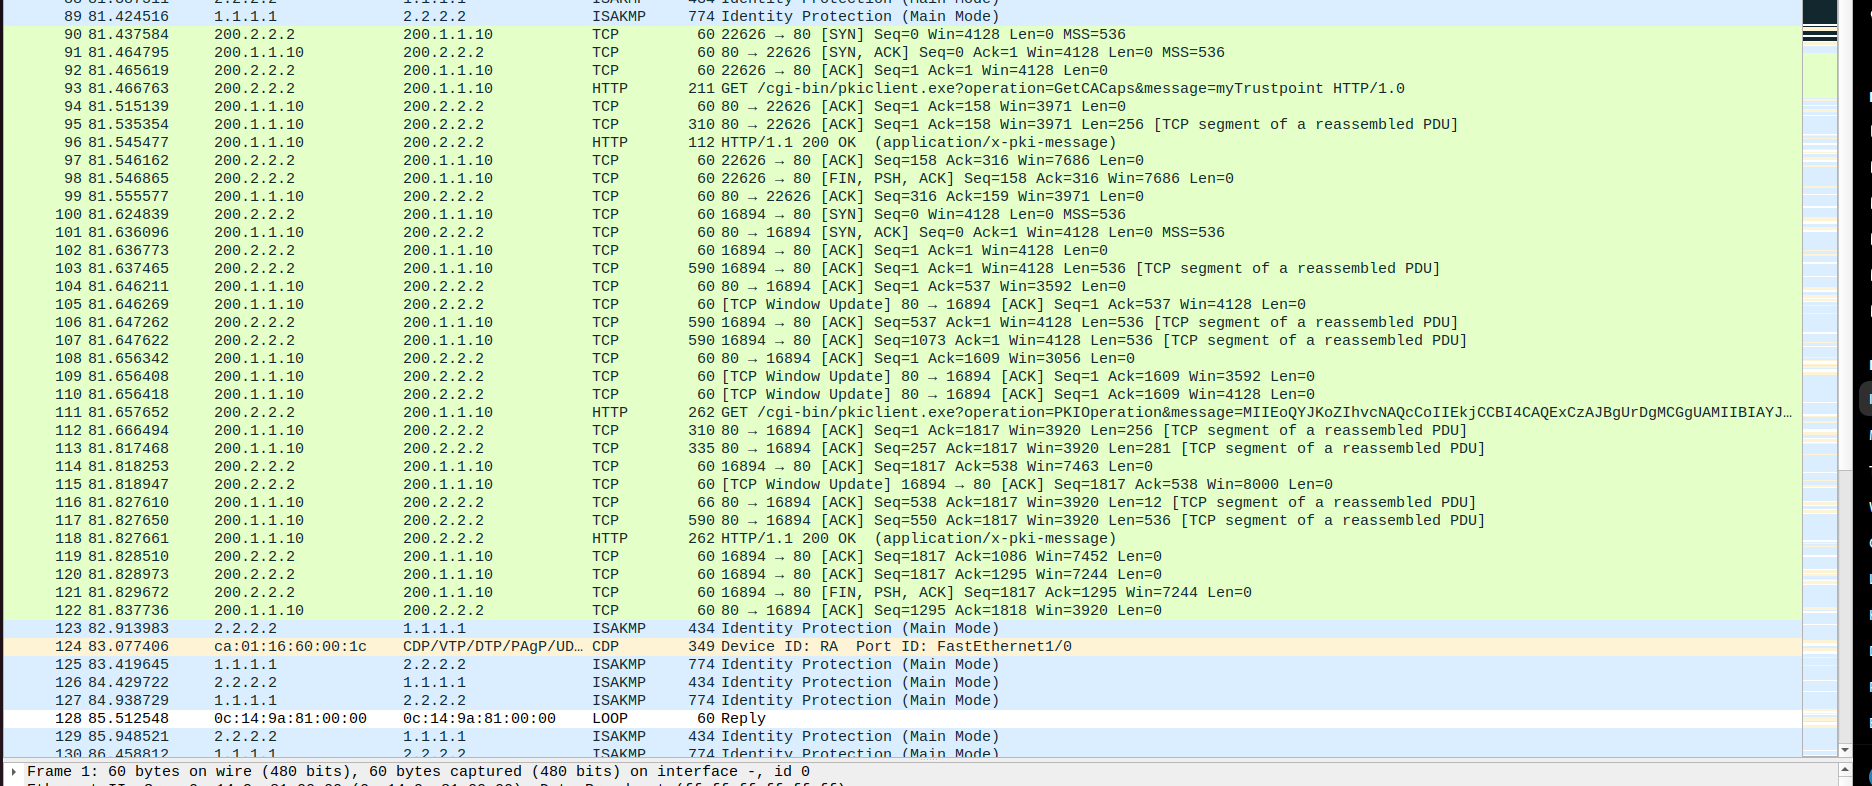
\includegraphics[width=\linewidth]{../Images/revoked-scep-traffic.png}
\caption{SCEP-related traffic observed after certificate revocation}
\label{fig:revoked_scep}
\end{figure}

These messages are associated with certificate validation and trust verification operations performed before IPSec authentication.

The routers contact the CA to verify the validity of certificates and retrieve updated revocation information.

\subsubsection{Failed ISAKMP Negotiation}

While the routers attempted to establish the IPSec tunnel, repeated ISAKMP exchanges were observed.

\begin{figure}[H]
\centering
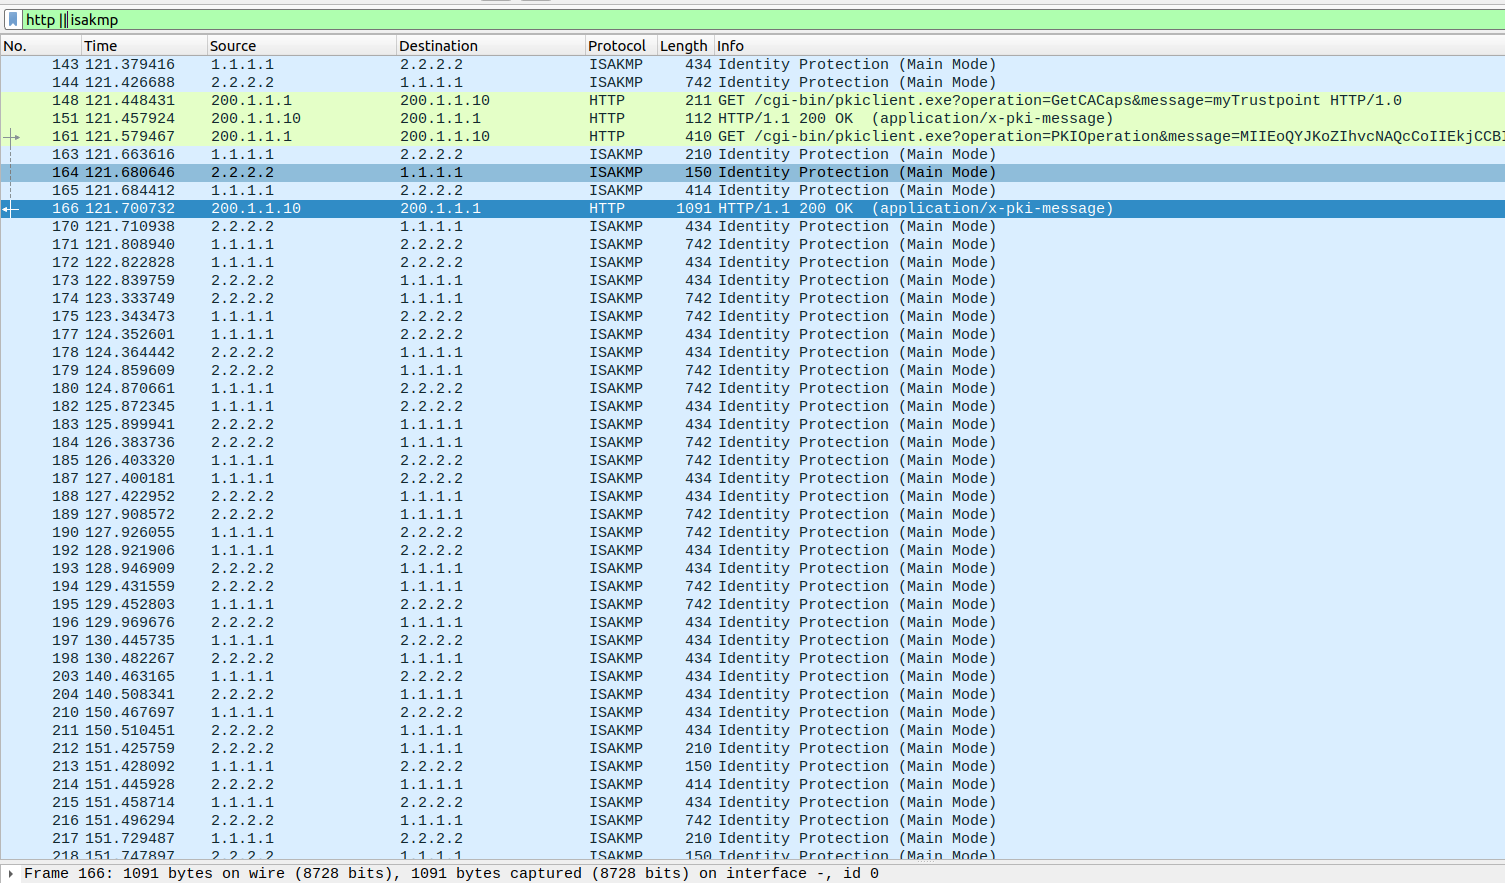
\includegraphics[width=\linewidth]{../Images/revoked-isakmp.png}
\caption{Repeated ISAKMP negotiation attempts after certificate revocation}
\label{fig:revoked_isakmp}
\end{figure}

The repeated ISAKMP packets indicate that the routers continuously attempt to establish an IKEv1 Security Association but fail during the authentication phase.

This behavior was confirmed using IOS verification commands.

\begin{verbatim}
R1#sh crypto isakmp sa 
IPv4 Crypto ISAKMP SA 
dst src state conn-id status 
1.1.1.1 2.2.2.2 MM_KEY_EXCH 1040 ACTIVE 
1.1.1.1 2.2.2.2 MM_KEY_EXCH 1038 ACTIVE 
1.1.1.1 2.2.2.2 MM_NO_STATE 1036 ACTIVE (deleted) 
1.1.1.1 2.2.2.2 MM_NO_STATE 1034 ACTIVE (deleted) 
2.2.2.2 1.1.1.1 MM_KEY_EXCH 1041 ACTIVE 
2.2.2.2 1.1.1.1 MM_NO_STATE 1039 ACTIVE (deleted) 
2.2.2.2 1.1.1.1 MM_NO_STATE 1037 ACTIVE (deleted) 

IPv6 Crypto ISAKMP SA
\end{verbatim}

The ISAKMP state remains in \texttt{MM\_KEY\_EXCH}, indicating that Main Mode negotiation does not complete successfully.

A successfully established tunnel would normally reach the \texttt{QM\_IDLE} state.

\subsubsection{Absence of IPSec Security Associations}

The IPSec SA database confirms that no operational IPSec tunnel was created.

\begin{verbatim}
R1#sh crypto ipsec sa 

interface: Tunnel0 
  Crypto map tag: Tunnel0-head-0, local addr 1.1.1.1 
  
  protected vrf: (none) 
  local ident (addr/mask/prot/port): (0.0.0.0/0.0.0.0/0/0) 
  remote ident (addr/mask/prot/port): (0.0.0.0/0.0.0.0/0/0) 
  current_peer 2.2.2.2 port 500 
   PERMIT, flags={origin_is_acl,} #pkts encaps: 0, 
  #pkts encrypt: 0, #pkts digest: 0 #pkts decaps: 0, 
  #pkts decrypt: 0, #pkts verify: 0 #pkts compressed: 0, 
  #pkts decompressed: 0 #pkts not compressed: 0, 
  #pkts compr. failed: 0 #pkts not decompressed: 0, 
  #pkts decompress failed: 0 
  #send errors 0, #recv errors 0 
  
  local crypto endpt.: 1.1.1.1, remote crypto endpt.: 2.2.2.2 
  plaintext mtu 1500, path mtu 1500, ip mtu 1500, ip mtu idb 
GigabitEthernet0/0 
  current outbound spi: 0x0(0) 
  PFS (Y/N): N, DH group: none 
  
  inbound esp sas: 
  
  inbound ah sas: 
  
  inbound pcp sas: 
  
  outbound esp sas: 
  
  outbound ah sas: 
  
  outbound pcp sas: 
  
R1#
\end{verbatim}

The counters remain at zero because IPSec encryption was never activated.

Additionally, no ESP Security Associations were present:

\begin{verbatim}
inbound esp sas:
outbound esp sas:
\end{verbatim}

This confirms that Phase 2 IPSec negotiation could not be completed.

\subsubsection{Explanation of Communication Failure}

Communication fails because the certificates used by R1 and R2 were revoked by the Certification Authority.

After reboot, the routers verify certificate validity during IKEv1 authentication. The CA indicates that the peer certificates are no longer trusted because they are listed in the Certificate Revocation List (CRL).

As a result:

\begin{itemize}
\item RSA signature authentication fails
\item IKEv1 Main Mode negotiation cannot complete
\item ISAKMP Security Associations are not successfully established
\item IPSec Security Associations are never created
\item ESP encrypted traffic cannot be generated
\item ICMP communication between PC1 and PC2 fails
\end{itemize}

The experiment demonstrates the importance of certificate revocation in PKI-based IPSec infrastructures, ensuring that compromised or invalid certificates cannot be used to establish trusted VPN connections.

\section{IPSec with IKEv2}

\subsection{Introduction}

This section describes the configuration and analysis of an IPSec VPN using IKEv2 authentication with pre-shared keys. The objective is to establish a protected tunnel between routers R1 and R2 through the intermediate router RA and analyze the establishment and operation of IKEv2 and IPSec Security Associations (SAs).

\subsection{IKEv2 and IPSec Configuration Verification}

The IKEv2 and IPSec configuration was verified on both R1 and R2 using IOS verification commands.

The following elements were validated:

\begin{itemize}
    \item IKEv2 proposals defining AES-CBC-256 encryption, SHA512 integrity, SHA512 PRF, and Diffie-Hellman Group 16;
    \item IKEv2 policies associated with the configured proposals;
    \item IPSec transform sets and profiles used for tunnel protection;
    \item active IPSec Security Associations and encapsulation parameters.
\end{itemize}

Figures~\ref{fig:ikev2_proposal}, \ref{fig:ikev2_policy}, \ref{fig:ipsec_profile}, and \ref{fig:ipsec_sa} present the verification outputs collected from both routers.

%------------------------------------------------
% IKEv2 Proposal
%------------------------------------------------

\begin{figure}[H]
    \centering

    \begin{minipage}{0.49\textwidth}
        \centering
        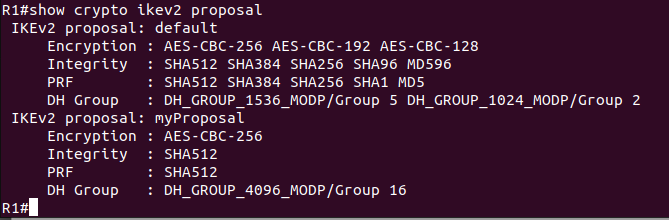
\includegraphics[width=\textwidth]{../Images/show crypto ikev2 prop R1.png}
        \caption*{R1}
    \end{minipage}
    \hfill
    \begin{minipage}{0.49\textwidth}
        \centering
        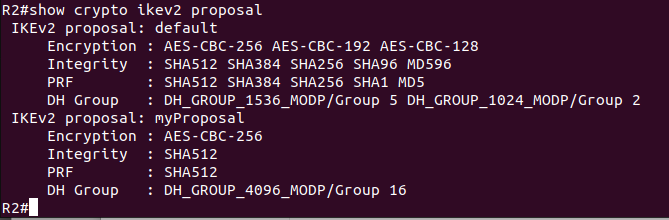
\includegraphics[width=\textwidth]{../Images/show crypto ikev2 prop R2.png}
        \caption*{R2}
    \end{minipage}

    \caption{IKEv2 proposal verification}
    \label{fig:ikev2_proposal}

\end{figure}

%------------------------------------------------
% IKEv2 Policy
%------------------------------------------------

\begin{figure}[H]
    \centering

    \begin{minipage}{0.49\textwidth}
        \centering
        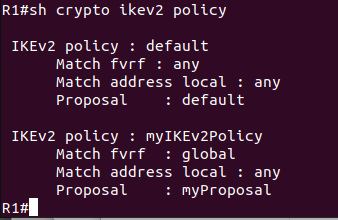
\includegraphics[width=\textwidth]{../Images/sh crypto policy R1.png}
        \caption*{R1}
    \end{minipage}
    \hfill
    \begin{minipage}{0.49\textwidth}
        \centering
        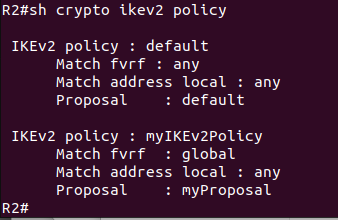
\includegraphics[width=\textwidth]{../Images/sh crypto policy R2.png}
        \caption*{R2}
    \end{minipage}

    \caption{IKEv2 policy verification}
    \label{fig:ikev2_policy}

\end{figure}

%------------------------------------------------
% IPSec Profile
%------------------------------------------------

\begin{figure}[H]
    \centering

    \begin{minipage}{0.49\textwidth}
        \centering
        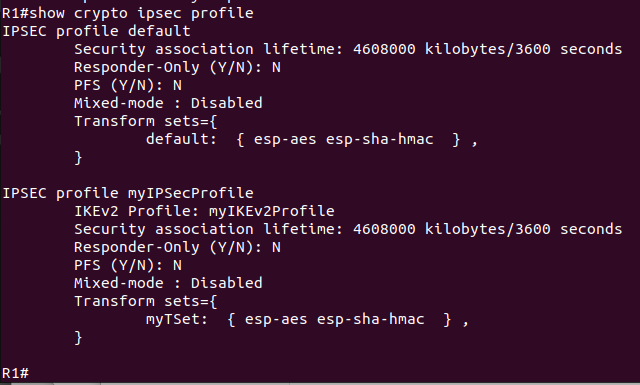
\includegraphics[width=\textwidth]{../Images/sh crypto ipsec profile R1.png}
        \caption*{R1}
    \end{minipage}
    \hfill
    \begin{minipage}{0.49\textwidth}
        \centering
        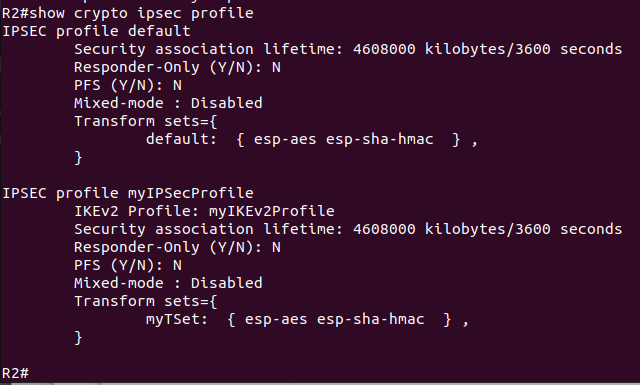
\includegraphics[width=\textwidth]{../Images/sh crypto ipsec profile R2.png}
        \caption*{R2}
    \end{minipage}

    \caption{IPSec profile verification}
    \label{fig:ipsec_profile}

\end{figure}

%------------------------------------------------
% IPSec SA
%------------------------------------------------

\begin{figure}[H]
    \centering

    \begin{minipage}{0.49\textwidth}
        \centering
        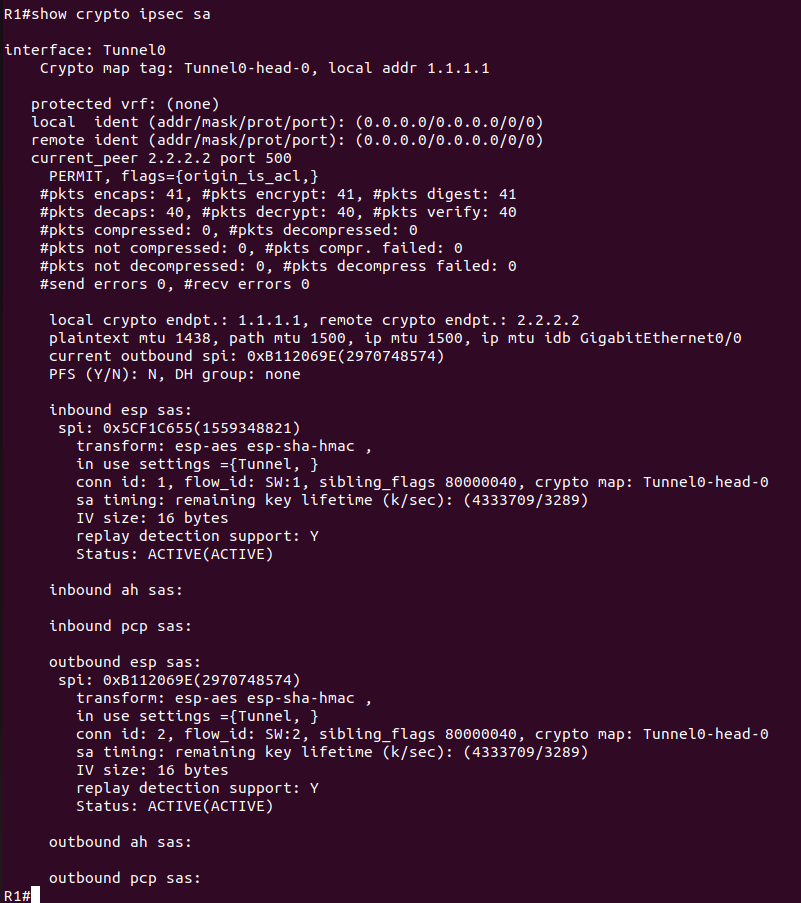
\includegraphics[width=\textwidth]{../Images/sh crypto ipsec sa R1.png}
        \caption*{R1}
    \end{minipage}
    \hfill
    \begin{minipage}{0.49\textwidth}
        \centering
        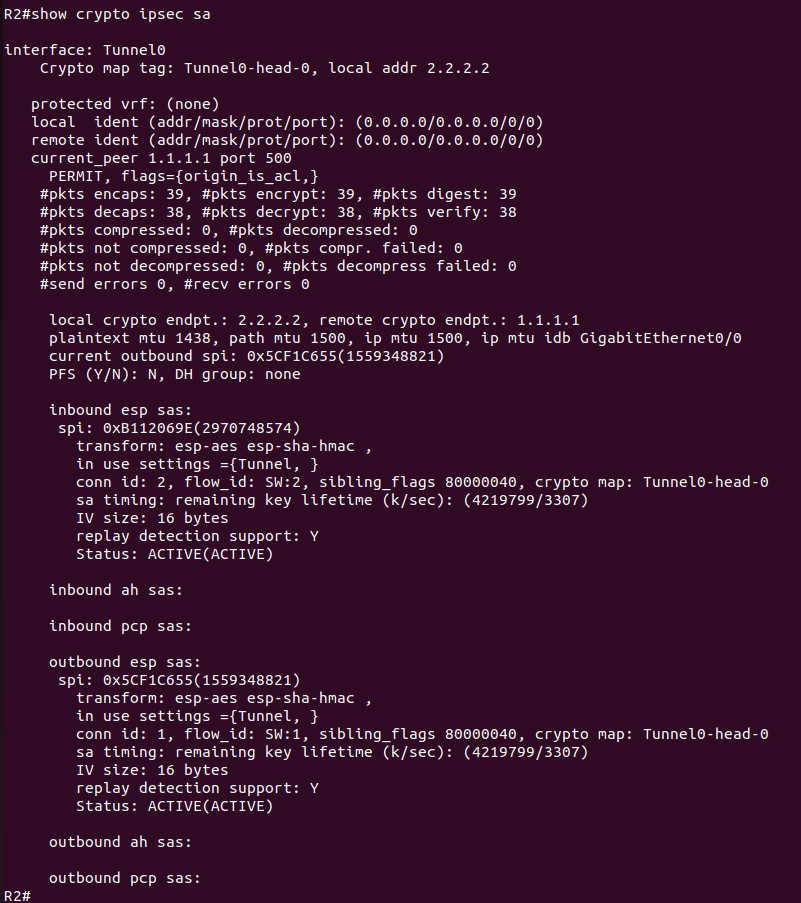
\includegraphics[width=\textwidth]{../Images/sh crypto ipsec sa R2.png}
        \caption*{R2}
    \end{minipage}

    \caption{Active IPSec Security Associations}
    \label{fig:ipsec_sa}

\end{figure}

The verification outputs confirm that the tunnel was successfully established and that encrypted traffic was being encapsulated and decapsulated through ESP Security Associations.

\subsection{Tunnel Establishment and Connectivity Test}

After configuration, end-to-end connectivity between PC1 and PC2 was verified using ICMP echo requests.

Successful communication confirmed that:
\begin{itemize}
    \item the IPSec tunnel was operational;
    \item encrypted traffic was correctly forwarded between endpoints;
    \item routing across the protected tunnel was functional.
\end{itemize}

Figure~\ref{fig:ping_test} shows successful ICMP communication between the end hosts through the IPSec tunnel.

\begin{figure}[H]
    \centering
    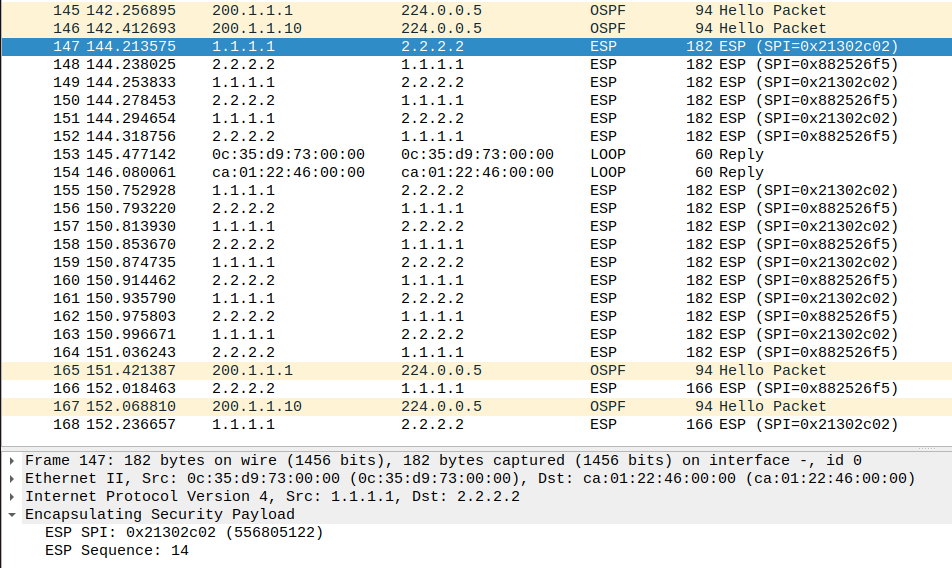
\includegraphics[width=0.7\textwidth]{../Images/ping IKEv2 pc to pc.png}
    \caption{Successful ICMP connectivity between PC1 and PC2}
    \label{fig:ping_test}
\end{figure}

\subsection{Analysis of IKE\_SA\_INIT Exchange}

Traffic captures were obtained on interface G0/0 of R1 during tunnel establishment.

The IKE\_SA\_INIT exchange is responsible for:
\begin{itemize}
    \item negotiation of cryptographic algorithms;
    \item exchange of Diffie-Hellman public values;
    \item generation of shared secret material;
    \item exchange of nonces;
    \item establishment of the initial IKE Security Association.
\end{itemize}

Figure~\ref{fig:ike_auth_content} presents the captured IKEv2 exchange messages.

\begin{figure}[H]
    \centering
    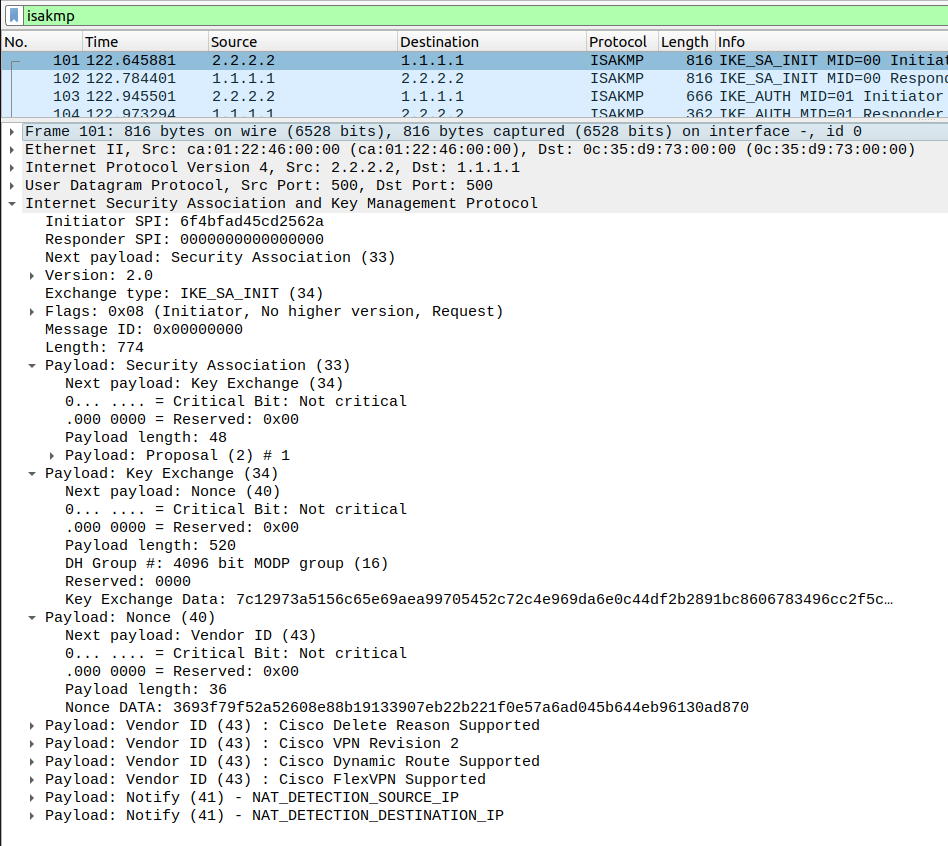
\includegraphics[width=\textwidth]{../Images/Content of INIT IKEv2.png}
    \caption{Contents of the IKE\_SA\_INIT exchange}
    \label{fig:ike_auth_content}
\end{figure}

\begin{figure}[H]
    \centering
    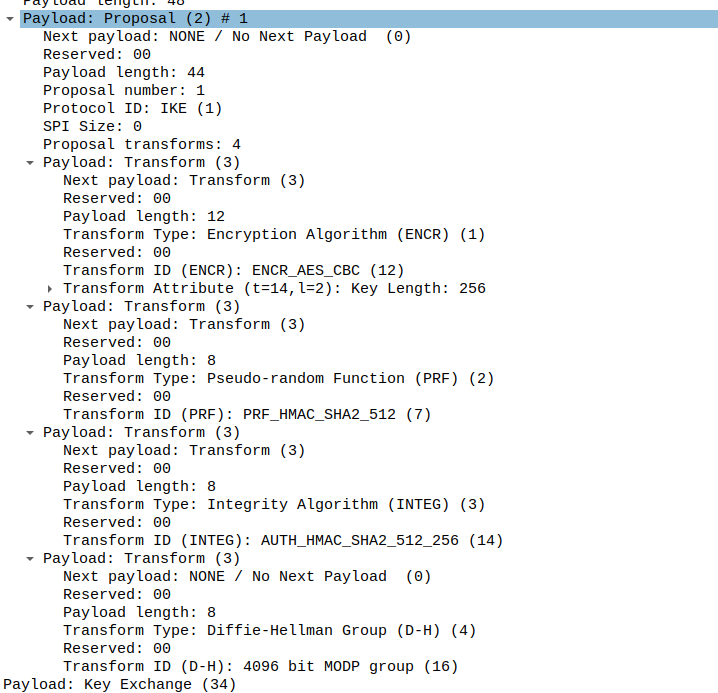
\includegraphics[width=\textwidth]{../Images/IKEv2 INIT payload expanded.png}
    \caption{Content of the payload: Proposal in the IKE\_SA\_INIT packet}
    \label{fig:ike_auth_content}
\end{figure}

The capture shows the Security Parameter Indexes (SPIs), Security Association proposals, Diffie-Hellman key exchange payloads, and nonce payloads exchanged between both peers.

The negotiated proposal includes:
\begin{itemize}
    \item AES-CBC-256 encryption;
    \item SHA2-512 integrity protection;
    \item SHA2-512 pseudo-random function (PRF);
    \item Diffie-Hellman Group 16.
\end{itemize}

The nonce payloads contribute entropy to the key generation process and ensure freshness of the exchange, protecting against replay attacks.

\subsection{SA Deletion and Re-establishment}

The command \texttt{clear crypto session} was executed to remove the active Security Associations and force a new negotiation process.

Wireshark captures show the deletion of the existing SAs followed by the establishment of new IKEv2 and IPSec Security Associations.

\begin{figure}[H]
    \centering
    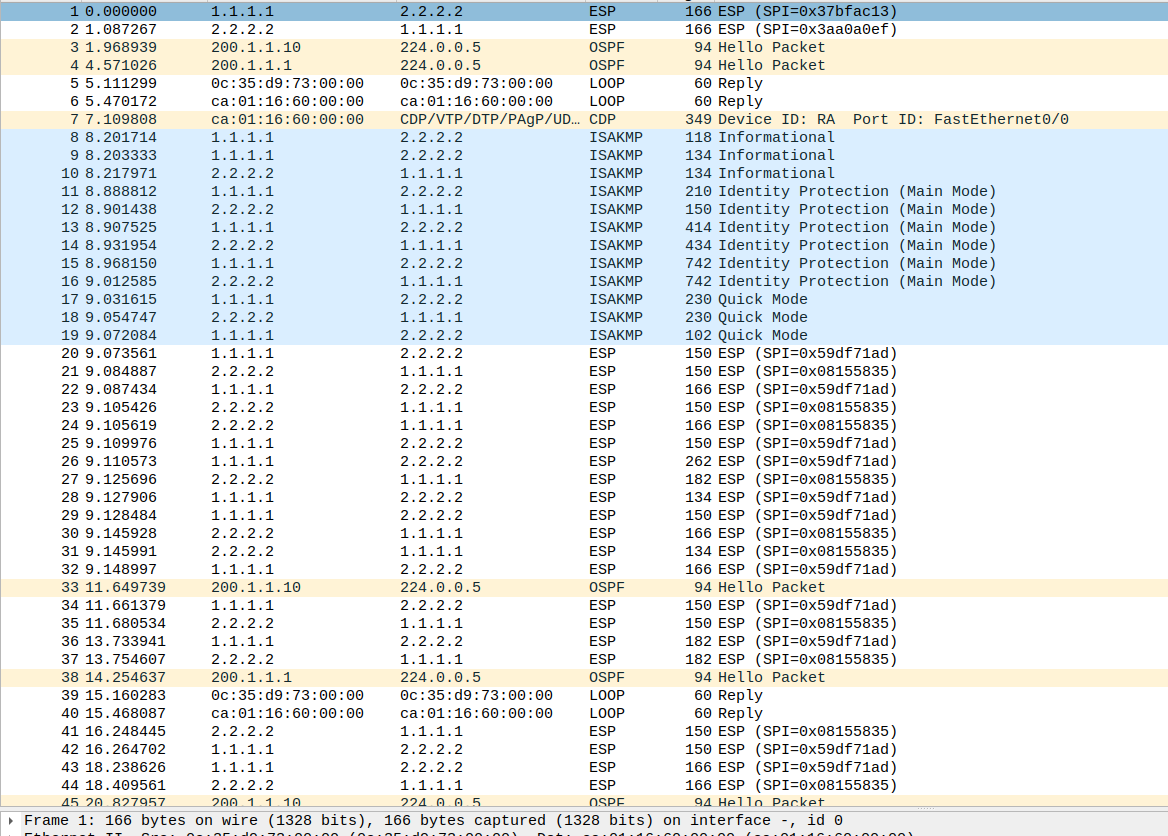
\includegraphics[width=\textwidth]{../Images/clear session msgs.png}
    \caption{Deletion and re-establishment of IKEv2 Security Associations after 
    clearing the crypto session, showing Informational deletion followed by new 
    IKE\_SA\_INIT and IKE\_AUTH exchanges}
    \label{fig:sa_reestablishment}
\end{figure}

After the previous SAs were removed, new IKE\_SA\_INIT and IKE\_AUTH exchanges were observed, resulting in the creation of new SPIs and new IPSec Security Associations.

The results confirm that IPSec tunnel establishment using IKEv2 was successfully achieved between R1 and R2.

The analysis of Wireshark captures demonstrated:
\begin{itemize}
    \item negotiation of cryptographic algorithms during IKE\_SA\_INIT;
    \item exchange of Diffie-Hellman values and nonces;
    \item encrypted peer authentication during IKE\_AUTH;
    \item successful creation of IPSec Security Associations;
    \item successful deletion and recreation of SAs after clearing the crypto session.
\end{itemize}

Cisco IOS verification commands further confirmed the operational state of the tunnel, the establishment of OSPF adjacency through Tunnel0, and the correct operation of encrypted ESP traffic.

\subsection{IKEv2 Security Association Rekeying}

To analyze the IKEv2 rekeying process, the lifetime of the IKEv2 Security Association was reduced to 180 seconds on R2 using the following configuration:

\begin{verbatim}
crypto ikev2 profile myIKEv2Profile
 lifetime 180
\end{verbatim}

After applying the configuration, the existing Security Associations were cleared using the \texttt{clear crypto session} command, allowing a new IKEv2 SA to be established with the updated lifetime.

Wireshark captures were obtained during the rekeying process. Figure~\ref{fig:ikev2_rekey_messages} presents the exchanged messages associated with IKEv2 rekeying.

\begin{figure}[H]
    \centering
    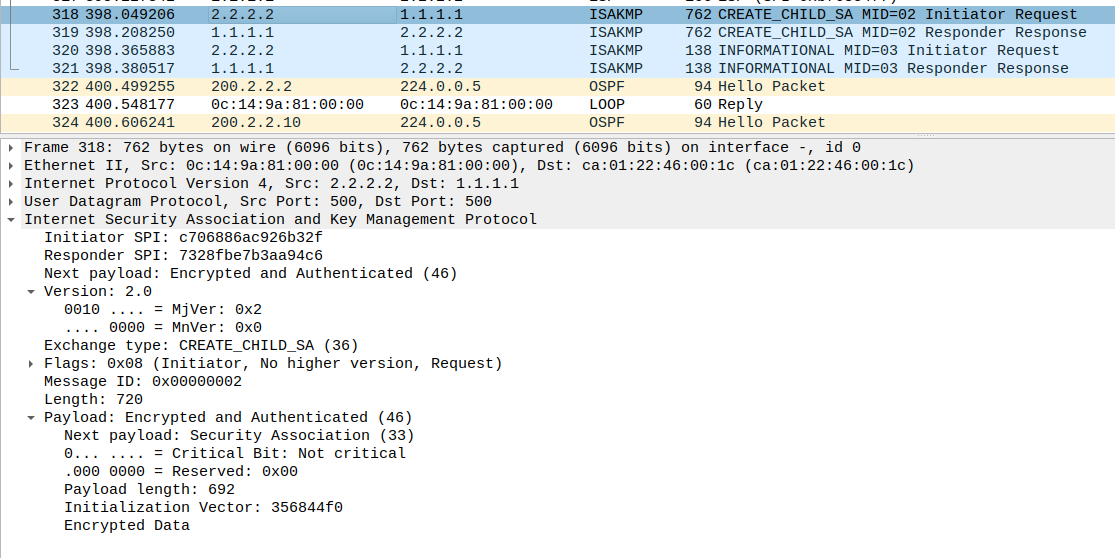
\includegraphics[width=\textwidth]{../Images/IKEv2 rekeying CHILD SA msg.png}
    \caption{IKEv2 rekeying messages captured in Wireshark}
    \label{fig:ikev2_rekey_messages}
\end{figure}

The captures show that the rekeying procedure does not restart the tunnel establishment from scratch. No new IKE\_SA\_INIT exchange was observed during rekeying. Instead, the process occurs through protected exchanges within the existing secure channel.

The CREATE\_CHILD\_SA exchange is responsible for generating fresh key material and establishing a new Security Association while the previous one is still active. This allows rekeying to occur without interrupting tunnel connectivity.

The evolution of the IKEv2 Security Association was verified using the \texttt{show crypto ikev2 sa detailed} command. Figure~\ref{fig:ikev2_sa_rekey} shows the Security Association state before and after rekeying.

\begin{figure}[H]
    \centering
    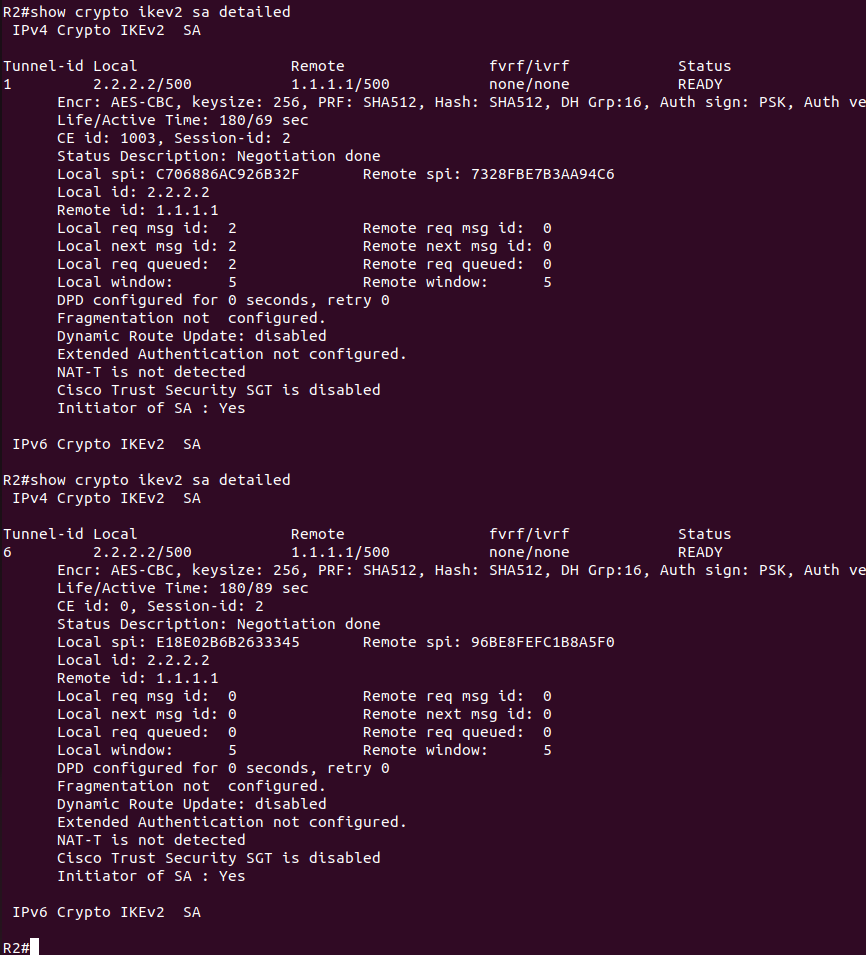
\includegraphics[width=\textwidth]{../Images/sh crypto detailed evolution.png}
    \caption{Evolution of the IKEv2 Security Association during rekeying}
    \label{fig:ikev2_sa_rekey}
\end{figure}

The outputs show that rekeying generated new local and remote SPIs while preserving the negotiated cryptographic algorithms and parameters. Additionally, the SA lifetime was refreshed after rekeying, confirming the successful establishment of a new IKEv2 Security Association.

The change in Tunnel-id, from 1 to 6, and SPI values demonstrates that the previous Security Association was replaced by a newly negotiated association.

\subsection{IPSec Security Association Rekeying}

To analyze the IPSec Security Association rekeying process, the IPSec SA lifetime was reduced to 120 seconds on R1 using the following configuration:

\begin{verbatim}
crypto ipsec profile myIPSecProfile
 set security-association lifetime seconds 120
\end{verbatim}

After saving the configuration, router R1 was restarted to ensure that the updated lifetime was applied to newly established IPSec Security Associations.

Wireshark captures were obtained during the rekeying process. Figure~\ref{fig:ipsec_rekey_messages} presents the exchanged messages associated with IPSec SA rekeying.

\begin{figure}[H]
    \centering
    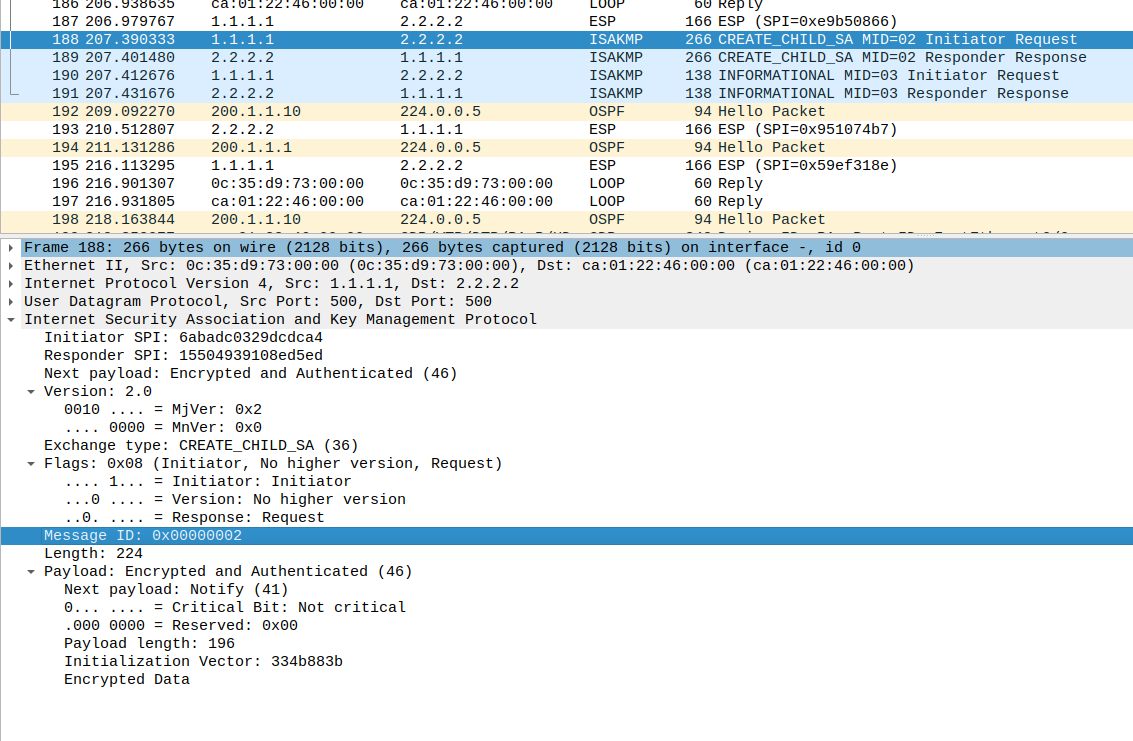
\includegraphics[width=\textwidth]{../Images/IKEv2 CHILD_SA msg ipsec.png}
    \caption{IPSec Security Association rekeying captured in Wireshark}
    \label{fig:ipsec_rekey_messages}
\end{figure}

Although both IKEv2 SA rekeying and IPSec SA rekeying use CREATE\_CHILD\_SA exchanges, the affected Security Associations differ. During IKEv2 SA rekeying, the IKE Security Association itself is replaced and new IKE SPIs are generated. During IPSec SA rekeying, only the ESP CHILD\_SA is replaced while the IKEv2 Security Association remains active.

The evolution of the IPSec Security Associations was verified using the \texttt{show crypto ipsec sa} command. Figure~\ref{fig:ipsec_sa_rekey} presents the Security Association state before and after rekeying.

\begin{figure}[H]
    \centering

    \begin{minipage}{0.49\textwidth}
        \centering
        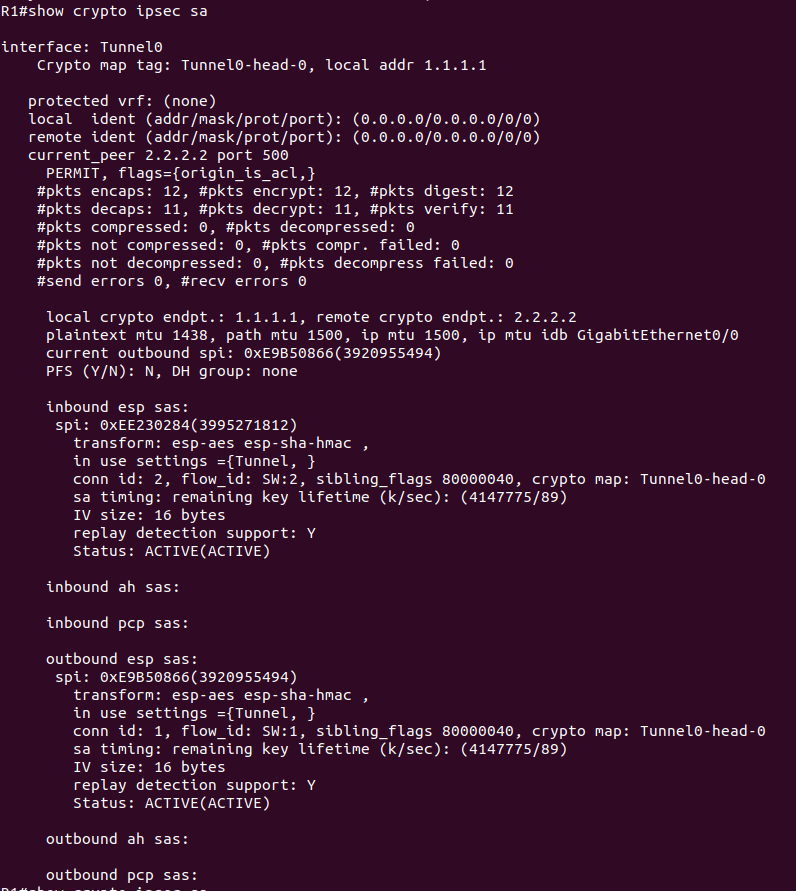
\includegraphics[width=\textwidth]{../Images/IKEv2 ipsec before rekeying.png}
        \caption*{Before rekeying}
    \end{minipage}
    \hfill
    \begin{minipage}{0.49\textwidth}
        \centering
        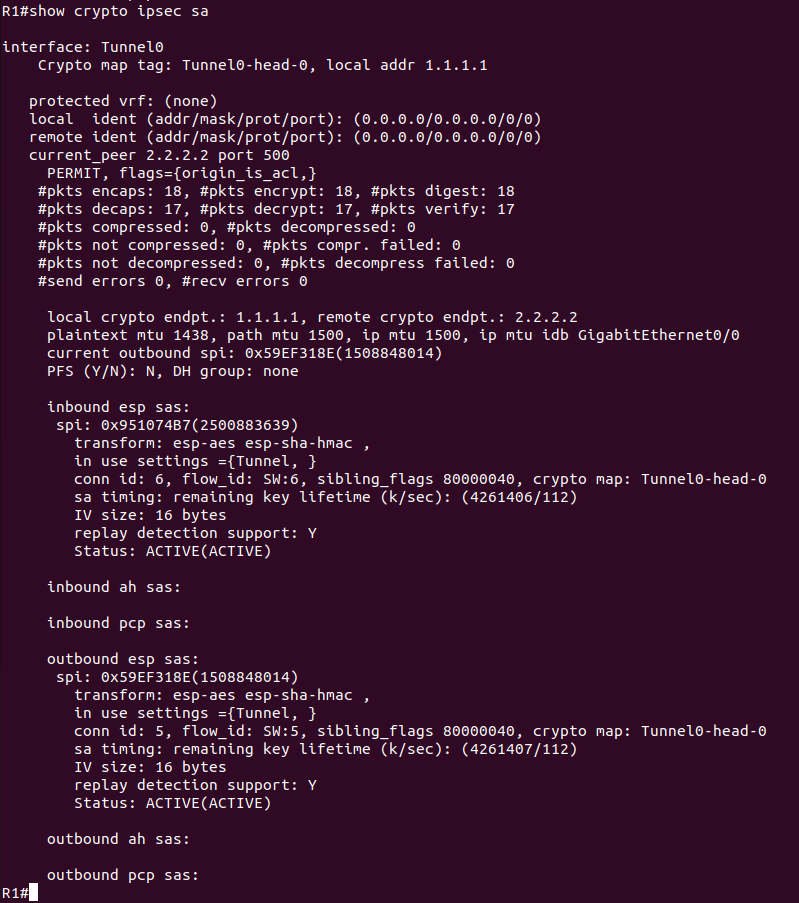
\includegraphics[width=\textwidth]{../Images/IKEv2 ipsec after rekeying.png}
        \caption*{After rekeying}
    \end{minipage}

    \caption{Evolution of the IPSec Security Associations during rekeying}
    \label{fig:ipsec_sa_rekey}

\end{figure}

The outputs show that the inbound and outbound ESP SPIs changed after rekeying, confirming that new IPSec Security Associations were created. Additionally, the Security Association lifetime was refreshed after rekeying while the negotiated cryptographic parameters remained unchanged.

The packet counters continued increasing throughout the process, demonstrating that encrypted traffic continued uninterrupted during the IPSec SA rekeying operation.

Unlike IKEv2 Security Association rekeying, which replaces the IKE SA itself, IPSec rekeying only replaces the CHILD\_SA used for ESP traffic protection while preserving the already established IKEv2 Security Association.

\newpage

\section{DMVPN Phase 3}

The objective of this experiment was to configure and analyse a DMVPN Phase~3 
network using RIP, NHRP redirects, and NHRP shortcuts. The behaviour of DMVPN 
Phase~3 was compared with DMVPN Phase~1 and Phase~2 using Cisco IOS commands 
and Wireshark captures.

%------------------------------------------------------------
\subsection{Topology}
%------------------------------------------------------------

Figure~\ref{fig:topology} shows the network topology used in the experiment. 
Router R1 operated as the DMVPN hub, while R2 and R3 operated as spokes. The 
public underlay uses OSPF, while the overlay private network uses RIPv2.

\begin{figure}[H]
    \centering
    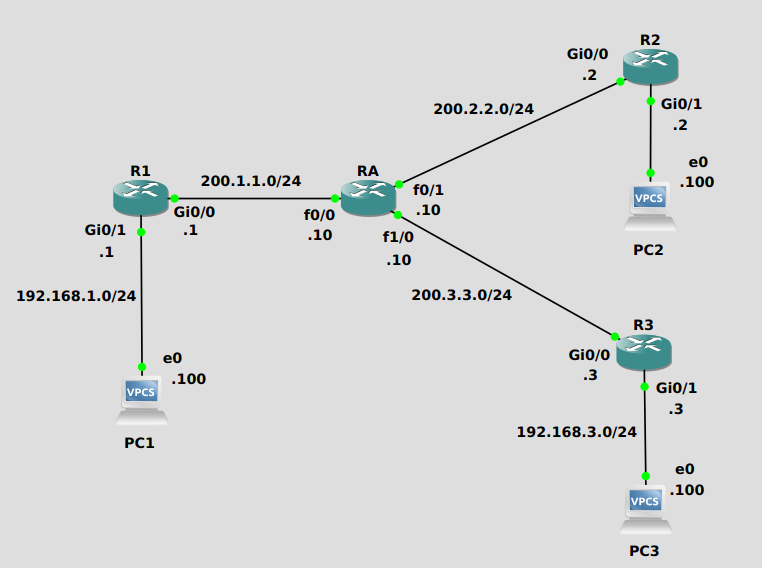
\includegraphics[width=0.6\linewidth]{../Images/topoly_DMVPN.png}
    \caption{DMVPN Phase 3 topology}
    \label{fig:topology}
\end{figure}

%------------------------------------------------------------
\subsection{DMVPN Phase 3 Configuration}
%------------------------------------------------------------

DMVPN Phase~3 was configured using mGRE tunnel interfaces on all routers, RIPv2 
in the overlay, NHRP redirects (\texttt{ip nhrp redirect}) on the hub, and NHRP 
shortcuts (\texttt{ip nhrp shortcut}) on the spokes, combined with route 
summarisation via \texttt{ip summary-address rip 0.0.0.0 0.0.0.0} on the hub's 
tunnel interface.

%------------------------------------------------------------
\subsection{Role of \texttt{ip summary-address rip}}
%------------------------------------------------------------

This command causes R1 to advertise only a default route (\texttt{0.0.0.0/0}) to 
all spokes via RIP, instead of individual spoke subnets. Figure~\ref{fig:riproute} 
confirms that R2 learns only the default route via \texttt{10.10.10.1} and not 
\texttt{192.168.3.0/24} directly.

\begin{figure}[H]
    \centering
    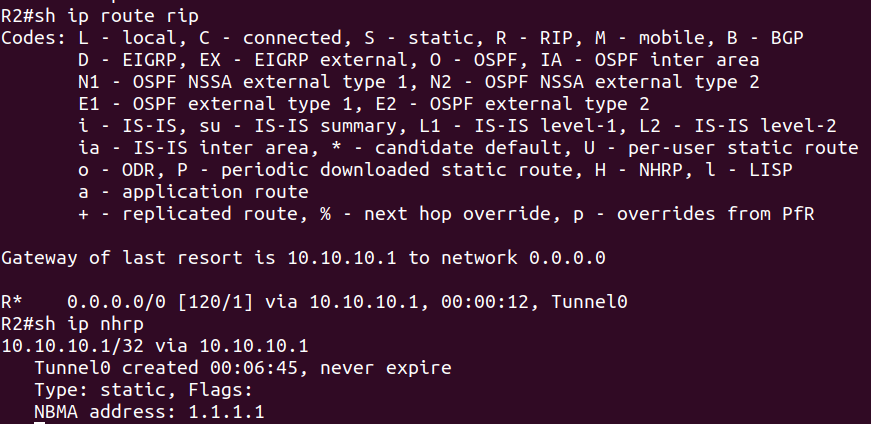
\includegraphics[width=0.85\linewidth]{../Images/iprouterip_R2.png}
    \caption{Default route learned through RIP at R2}
    \label{fig:riproute}
\end{figure}

Because spokes only hold a default route toward the hub, all initial 
spoke-to-spoke traffic transits R1, giving it the opportunity to issue NHRP 
redirects. When the command was temporarily removed, R1 advertised specific spoke 
subnets and R2 routed directly to R3 --- NHRP redirects were never triggered, 
confirming the command is a prerequisite for Phase~3 operation.

%------------------------------------------------------------
\subsection{Role of RIP Split Horizon}
%------------------------------------------------------------

RIP split horizon prevents R1 from re-advertising routes learned from one spoke 
back out the same mGRE tunnel interface toward other spokes. Without it, R2 and 
R3 would learn each other's subnets via the hub and route directly, bypassing R1 
entirely before NHRP shortcuts could be created. When split horizon was disabled 
with \texttt{no ip split-horizon} on R1's tunnel interface, specific spoke routes 
propagated to all spokes and no shortcuts were ever established, confirming that 
split horizon and \texttt{ip summary-address rip} must both be active for Phase~3 
to work correctly.

%------------------------------------------------------------
\subsection{OSPF vs RIP at the Public Network}
%------------------------------------------------------------

Two distinct routing protocol traffic types are visible at the public network 
links. OSPF Hello packets carry outer destination \texttt{224.0.0.5} and are 
sourced from physical underlay interfaces --- they are not GRE-encapsulated and 
maintain adjacencies solely in the underlay. RIP Response packets, by contrast, 
are GRE-encapsulated and carry outer loopback-to-loopback addresses (e.g., 
\texttt{1.1.1.1} $\rightarrow$ \texttt{2.2.2.2}), travelling inside the mGRE 
overlay to distribute private subnet reachability between sites. OSPF is never 
aware of the private subnets, and RIP is never visible on the underlay.

%------------------------------------------------------------
\subsection{NHRP Redirects and Shortcuts}
%------------------------------------------------------------

Initially R2 only knows the hub's NBMA address. When PC2 pings PC3, R2 forwards 
the first ICMP Echo Request to R1. R1 simultaneously forwards it to R3 and sends 
an NHRP Traffic Indication back to R2, identifying \texttt{10.10.10.3} as a 
destination reachable via a better path. Figure~\ref{fig:redirect} shows these 
Traffic Indication packets captured at the public network.

\begin{figure}[H]
    \centering
    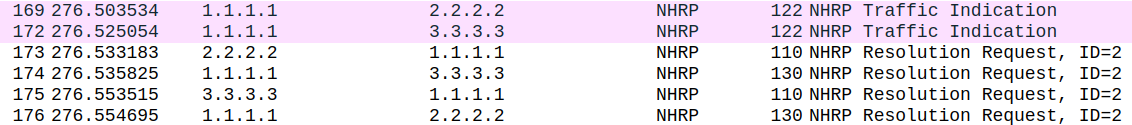
\includegraphics[width=0.9\linewidth]{../Images/trafficindic_wire.png}
    \caption{NHRP Traffic Indication packets generated by R1}
    \label{fig:redirect}
\end{figure}

R2 then sends an NHRP Resolution Request to resolve R3's NBMA address, carrying 
its own source NBMA (\texttt{2.2.2.2}) and protocol (\texttt{10.10.10.2}) 
addresses. R3 replies with its NBMA address (\texttt{3.3.3.3}). 
Figure~\ref{fig:resolution} shows this exchange, and Figure~\ref{fig:dmvpn} shows 
the resulting dynamic shortcut entry installed at R2.

\begin{figure}[H]
    \centering
    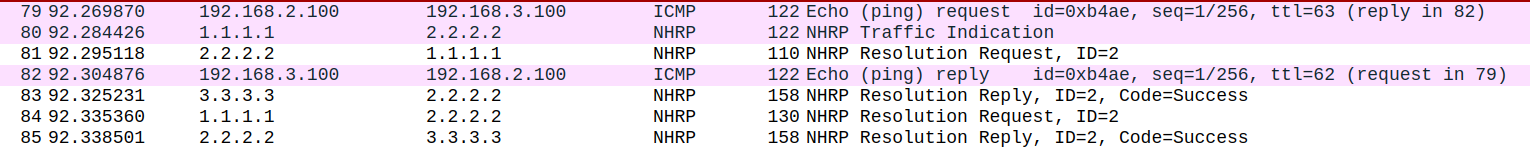
\includegraphics[width=0.9\linewidth]{../Images/wire2.png}
    \caption{NHRP Resolution Request and Reply}
    \label{fig:resolution}
\end{figure}

\begin{figure}[H]
    \centering
    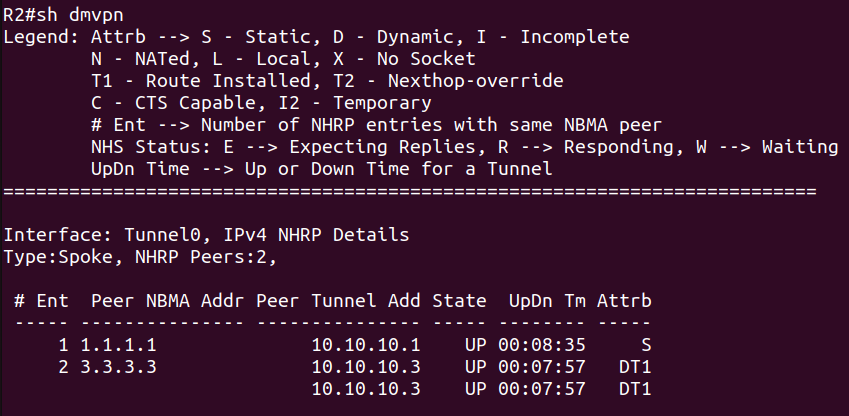
\includegraphics[width=0.75\linewidth]{../Images/sh_dmvpnR2.png}
    \caption{Dynamic DMVPN shortcut entry at R2}
    \label{fig:dmvpn}
\end{figure}

All subsequent packets from PC2 to PC3 are sent directly to R3's NBMA address, 
as confirmed by the traceroute in Figure~\ref{fig:trace}.

%------------------------------------------------------------
\subsection{Traffic Analysis}
%------------------------------------------------------------

\begin{figure}[H]
    \centering
    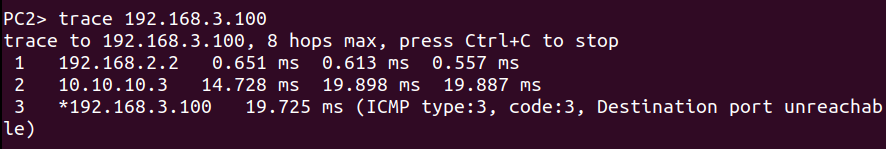
\includegraphics[width=0.75\linewidth]{../Images/tracePC2_PC3.png}
    \caption{Traceroute between spokes after shortcut creation}
    \label{fig:trace}
\end{figure}

The traceroute confirms that after the NHRP shortcut is established, packets 
travel directly between R2 and R3 without transiting R1.

%------------------------------------------------------------
\subsection{Comparison Between DMVPN Phases}
%------------------------------------------------------------

\textbf{Phase~1} uses point-to-point hub-to-spoke tunnels. All spoke-to-spoke 
traffic must transit R1 permanently --- simple to configure but does not scale.

\textbf{Phase~2} introduces mGRE on all routers. NHRP resolution allows direct 
spoke-to-spoke tunnels, but the routing protocol must preserve the original 
next-hop, requiring per-spoke routing entries on every spoke.

\textbf{Phase~3} decouples routing from NHRP via summarisation. Spokes need only 
a single default route toward the hub; NHRP redirects and shortcuts build direct 
paths on demand. Adding a new spoke requires no routing table changes on existing 
spokes, making Phase~3 the most scalable of the three.

%------------------------------------------------------------
\subsection{AI Comparison}
%------------------------------------------------------------

The AI correctly identified that \texttt{ip summary-address rip} injects a 
default route from hub to spokes and that NHRP redirects trigger spoke-to-spoke 
shortcut creation.

Two discrepancies were found experimentally. First, the AI described RIP split 
horizon as preventing routing loops in general, without identifying the specific 
Phase~3 consequence: that disabling it causes spokes to learn direct routes and 
bypass the hub before shortcuts are created. This was confirmed by the 
split-horizon experiment above. Second, the AI stated that the hub sends the NHRP 
redirect \emph{before} forwarding the packet. The Wireshark captures show the 
redirect and the forwarded packet occurring simultaneously, not sequentially.

\section{VRFs and BGP-MPLS L3VPNs}

\subsection{Introduction}

This laboratory exercise explored the implementation of a BGP/MPLS Layer 3 VPN using GNS3 and Cisco IOS routers. Two customer organizations (Blue and Red), each with two geographically separated sites, were interconnected through a provider MPLS backbone composed of PE and P routers. Virtual Routing and Forwarding (VRF) instances were used to isolate customer routing information, while MP-BGP distributed VPN routes and MPLS labels between PE routers. The objective of the exercise was to analyze how MPLS labels, VRFs, and MP-BGP cooperate to provide scalable and isolated Layer 3 VPN connectivity across a shared provider infrastructure.

\subsection{Ping Between Sites and Loopback Sourcing}

Connectivity between the sites of each organization was verified by executing sourced pings between the CE routers. Figure~\ref{fig:blue_ping} presents the successful ping from Blue1 to Blue2, and Figure~\ref{fig:red_ping} presents the successful ping from Red1 to Red2.
\begin{figure}[H]
    \centering
    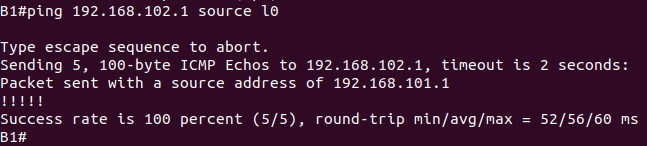
\includegraphics[width=\textwidth]{../Images/Ping Blue client vpn.png}
    \caption{Successful ping from Blue1 to Blue2}
    \label{fig:blue_ping}
\end{figure}

\begin{figure}[H]
    \centering
    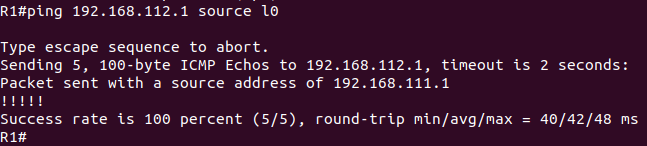
\includegraphics[width=\textwidth]{../Images/Ping Red client vpn.png}
    \caption{Successful ping from Red1 to Red2}
    \label{fig:red_ping}
\end{figure}

The pings are sourced from the loopback interfaces because these are the prefixes advertised into the VPN through the static routes redistributed into MP-BGP. The physical CE interface addresses (e.g. \texttt{10.10.1.100}) are local to the PE--CE segment and are never injected into the VRF routing table of the remote PE. A ping sourced from the physical interface would reach the destination but the reply would be dropped at the remote PE for lack of a return route. Sourcing from the loopback tests the actual end-to-end VPN path across the advertised prefixes.

\subsection{PE1 Routing Tables}

The routing architecture of PE1 was analyzed by inspecting the global routing table and the per-VRF routing tables. Figure~\ref{fig:pe1_global} presents the global table, and Figures~\ref{fig:pe1_vrf_blue} and~\ref{fig:pe1_vrf_red} present the VRF tables for the blue and red organizations respectively.

\begin{figure}[H]
    \centering
    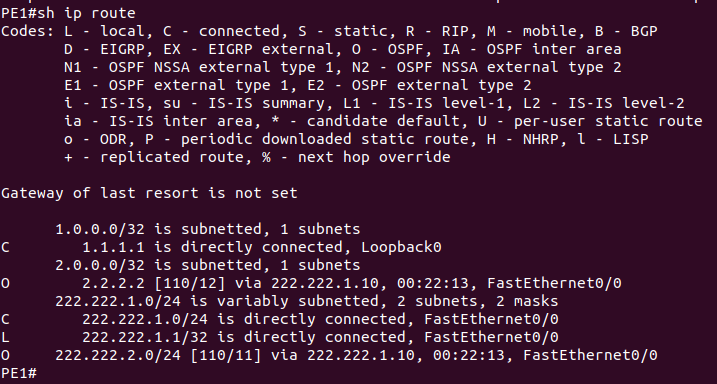
\includegraphics[width=\textwidth]{../Images/PE1 routing table.png}
    \caption{Global routing table of PE1, containing only provider infrastructure routes}
    \label{fig:pe1_global}
\end{figure}

The global routing table contains exclusively provider infrastructure routes: the directly connected provider links (\texttt{222.222.x.x}), the PE and P loopbacks learned via OSPF, and no customer prefixes whatsoever. This reflects the fundamental VRF isolation principle, customer routes exist only within their respective VRF instances and are completely invisible to the global forwarding plane.

\begin{figure}[H]
    \centering
    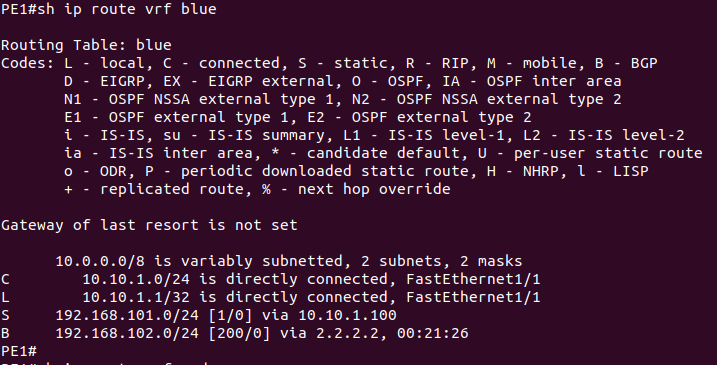
\includegraphics[width=\textwidth]{../Images/Blue vrf routing table PE1.png}
    \caption{Blue vrf routing table in PE1}
    \label{fig:pe1_vrf_blue}
\end{figure}

\begin{figure}[H]
    \centering
    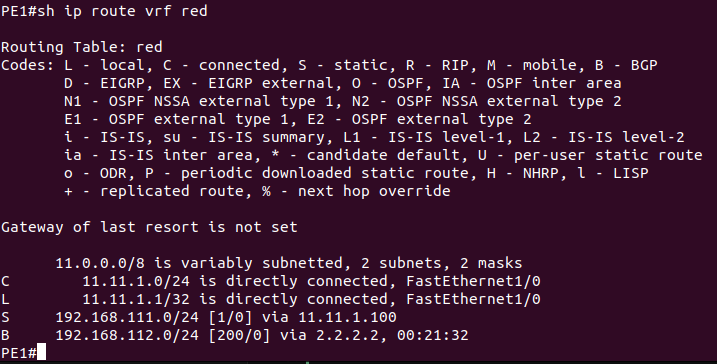
\includegraphics[width=\textwidth]{../Images/Red vrf routing table PE1.png}
    \caption{Red vrf routing table in PE1}
    \label{fig:pe1_vrf_red}
\end{figure}

The blue VRF routing table contains three categories of entries. The directly connected entry for \texttt{10.10.1.0/24} corresponds to the PE1--Blue1 segment. The static route for \texttt{192.168.101.0/24} via \texttt{10.10.1.100} was manually configured to reach Blue1's loopback and is redistributed into MP-BGP. The BGP route for \texttt{192.168.102.0/24} via \texttt{2.2.2.2} was learned from PE2 through the MP-BGP session, with PE2's loopback serving as the next hop resolved through the MPLS core. The red VRF table is symmetric, containing the equivalent entries for the red organization's address space.

The two organizations are isolated from each other because each VRF constitutes an independent routing and forwarding instance. Interfaces are explicitly bound to a single VRF, so incoming packets are looked up exclusively within that VRF's FIB. Furthermore, route import and export is governed by the Route Target extended community: the blue VRF is configured with \texttt{route-target both 1:1} and the red VRF with \texttt{route-target both 2:2}, meaning a route advertised by one organization is never imported into the other's VRF regardless of address overlap.

\subsection{MPLS Labels During Ping Analysis}

To analyze the MPLS label stack used within the provider network, Wireshark captures 
were obtained on both the PE1--P and P--PE2 links while executing 
\texttt{ping 192.168.102.1 source l0} from Blue1. Figures~\ref{fig:mpls_2_labels} 
and~\ref{fig:mpls_1_label} present the captured packets on each segment respectively.

\begin{figure}[H]
    \centering
    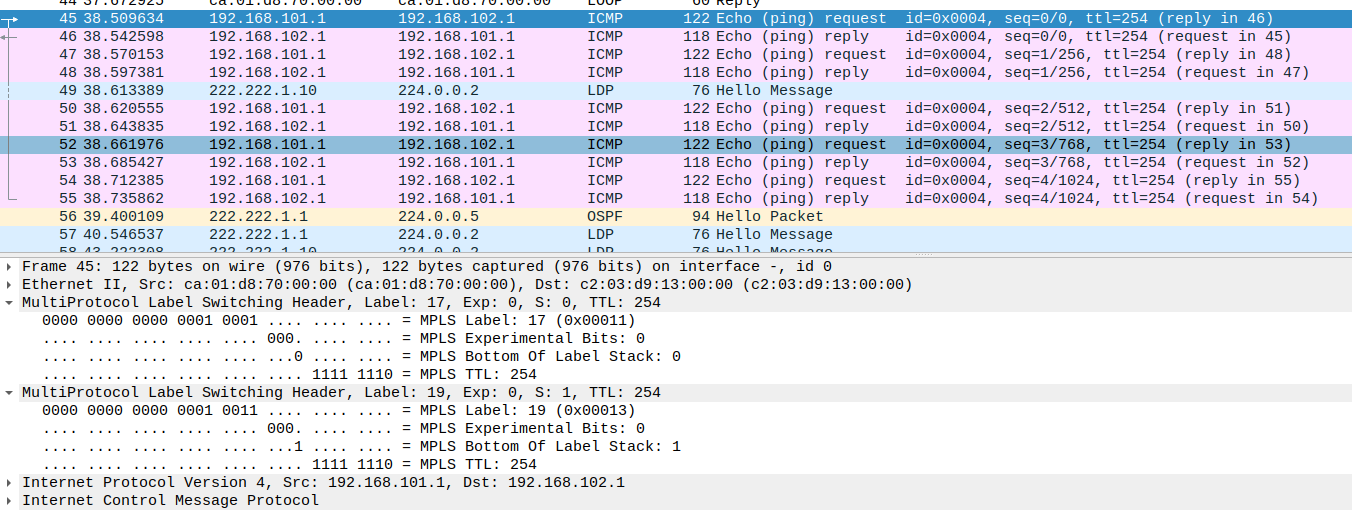
\includegraphics[width=\textwidth]{../Images/MPLS 2 labels ping Blue.png}
    \caption{Message captured between PE1 and P, displaying 2 labels}
    \label{fig:mpls_2_labels}
\end{figure}

\begin{figure}[H]
    \centering
    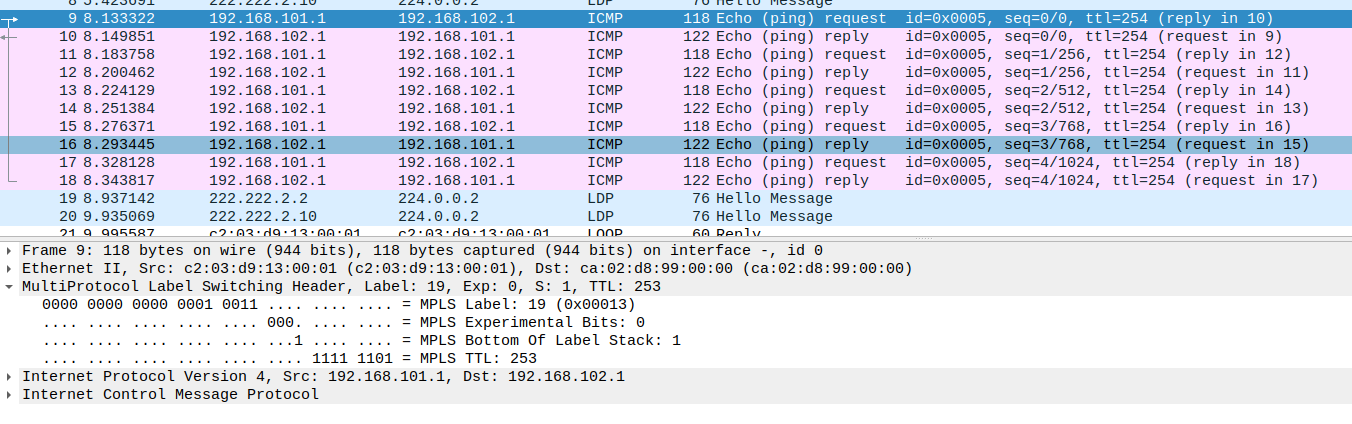
\includegraphics[width=\textwidth]{../Images/MPLS 1 label ping Blue.png}
    \caption{Message captured between P-PE2 displaying only 1 label}
    \label{fig:mpls_1_label}
\end{figure}

On the PE1--P segment, each ICMP packet carries a two-label MPLS stack. The outer 
label (value 17) is the transport label, distributed by LDP, and is used exclusively 
to switch the packet across the provider core toward PE2's loopback \texttt{2.2.2.2}. 
Its Bottom of Stack (S) bit is set to 0, indicating that additional labels follow 
beneath it in the stack. The inner label (value 19) is the VPN label, distributed by 
MP-BGP, and identifies the destination VRF at the egress PE. Its S bit is set to 1, 
marking it as the last label in the stack, after which the original IP packet begins.

It is important to note that the VPN label value 19 was not assigned by PE1, the 
ingress router, but rather by PE2, the egress router. In MPLS VPN, each PE assigns 
labels for the prefixes it advertises and communicates them to the remote PE via 
MP-BGP Update messages. PE2 assigned label 19 for prefix \texttt{192.168.102.0/24} 
and advertised it to PE1, which then imposes that label on all traffic destined for 
that prefix. This is confirmed by \texttt{show bgp vpnv4 unicast vrf blue 
192.168.102.0} on PE1 shown in Figure~\ref{fig:bgp_vpnv4}, where the outgoing label 
field shows the value received from PE2. The ingress PE is therefore always 
responsible for imposing a label that was assigned and advertised by the egress PE.

\begin{figure}[H]
    \centering
    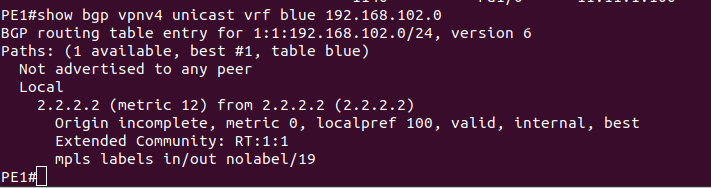
\includegraphics[width=\textwidth]{../Images/BGP vpnv4 vrf blue 192.168.102.0.png}
    \caption{BGP VPNv4 entry for prefix 192.168.102.0/24 at PE1, showing outgoing VPN label assigned by PE2}
    \label{fig:bgp_vpnv4}
\end{figure}


These label values are directly correlated with the MPLS forwarding table of PE1, 
shown in Figure~\ref{fig:mpls_pe1}. The entry for \texttt{2.2.2.2/32} shows outgoing 
label 17 via \texttt{FastEthernet0/0}, confirming that PE1 imposes the LDP transport 
label 17 to reach PE2's loopback through the P router. The VPN entry for 
\texttt{192.168.102.0/24[V]} confirms that traffic destined for the blue VRF prefix 
is forwarded with the label stack observed in the capture.

\begin{figure}[H]
    \centering
    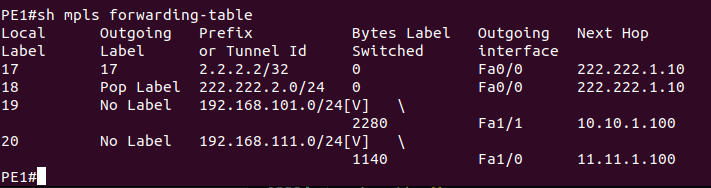
\includegraphics[width=\textwidth]{../Images/MPLS PE1 forwarding table.png}
    \caption{MPLS forwarding table of PE1, showing transport label 17 toward PE2 and VPN label entries}
    \label{fig:mpls_pe1}
\end{figure}

\begin{figure}[H]
    \centering
    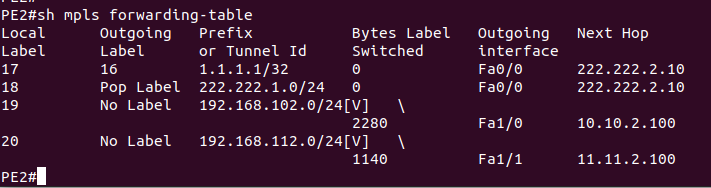
\includegraphics[width=\textwidth]{../Images/MPLS PE2 forwarding table.png}
    \caption{MPLS forwarding table of PE2, confirming PHP behavior and VPN label 19 mapping}
    \label{fig:mpls_pe2}
\end{figure}

On the P--PE2 segment, the packet carries only the VPN label (value 19), as shown in 
Figure~\ref{fig:mpls_1_label}. This results from Penultimate Hop Popping (PHP): the 
P router removes the outer transport label before forwarding the packet to PE2. PHP 
is implemented through LDP by advertising the implicit-null label for directly 
connected prefixes. PE2's LDP bindings confirm this behavior, as the local binding 
for \texttt{2.2.2.2/32} is \texttt{imp-null}, instructing the P router to pop the 
transport label before delivery. Consequently, PE2 receives the packet with only the 
inner VPN label, avoiding an additional label lookup.

PE2 uses the VPN label to identify the destination VRF and forward the packet to the 
correct CE. This is confirmed by PE2's MPLS forwarding table in 
Figure~\ref{fig:mpls_pe2}, where label 19 maps to 
\texttt{192.168.102.0/24[V]}. The \texttt{[V]} annotation indicates a VRF route, and 
the outgoing label field shows \texttt{No Label}, meaning PE2 removes the VPN label 
and forwards the packet natively into the blue VRF toward \texttt{10.10.2.100}. 
Similarly, the outer transport label value 17 observed on the PE1--P link was 
assigned by the P router and advertised to PE1 through LDP.

The VPN label ensures isolation between organizations, even when overlapping IP 
address spaces are used. Since forwarding at the egress PE is based on the VPN label 
rather than the destination IP address, packets with identical IP destinations can be 
delivered to different VRFs without ambiguity. The outer transport label is swapped 
at each LSR hop across the provider core, while the inner VPN label remains unchanged 
from ingress PE to egress PE, where it is finally removed.

\subsection{BGP Session Establishment and VPNv4 Route Advertisement}

To analyze the BGP Open and Update messages exchanged between PE1 and PE2, interface \texttt{f0/0} of PE2 was shut down and re-enabled while a Wireshark capture was running on the PE1--P link, forcing a new BGP session to be established. 

Figure~\ref{fig:bgp_open_pe1} presents the BGP Open messages sent by PE1.

\begin{figure}[H]
    \centering
    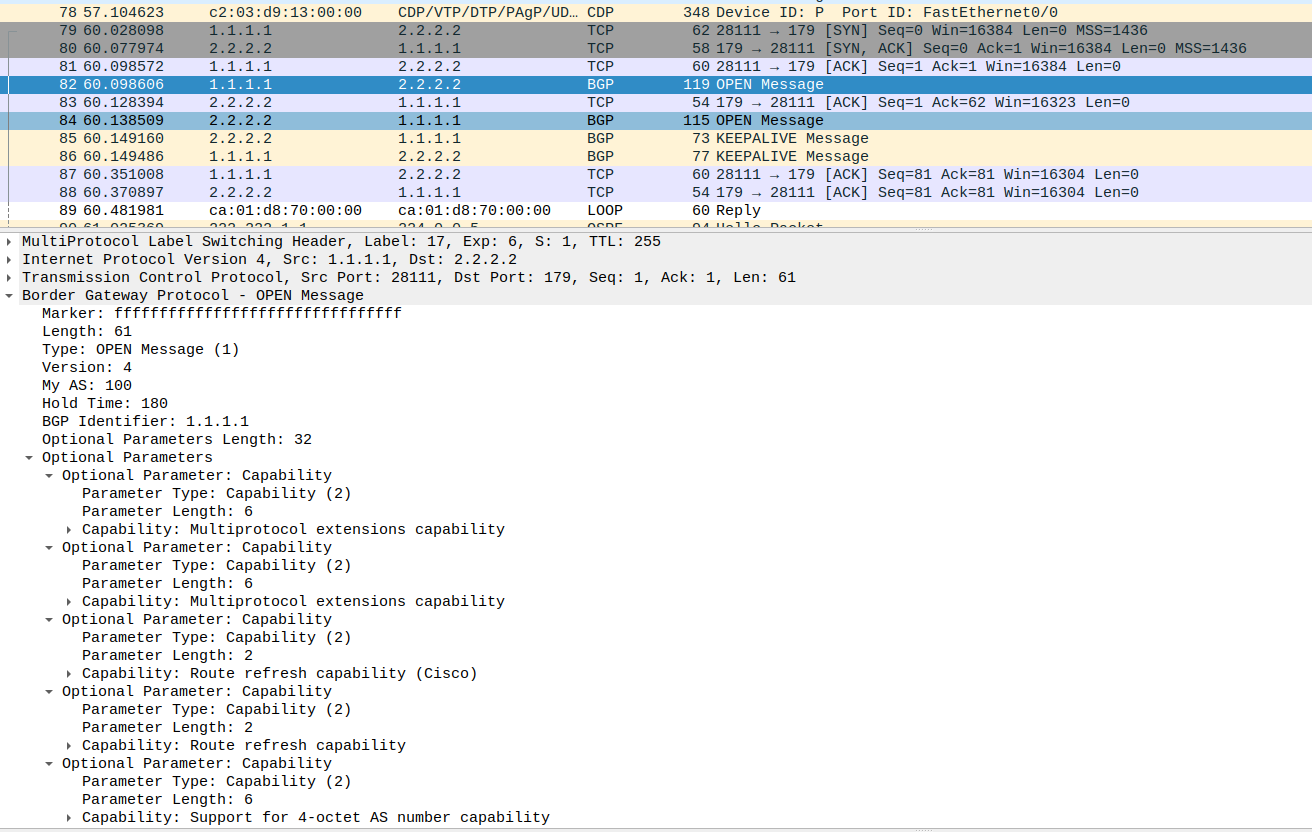
\includegraphics[width=\textwidth]{../Images/BGP open msgs.png}
    \caption{Open messages exchanged}
    \label{fig:bgp_open_pe1}
\end{figure}


\begin{figure}[H]
    \centering
    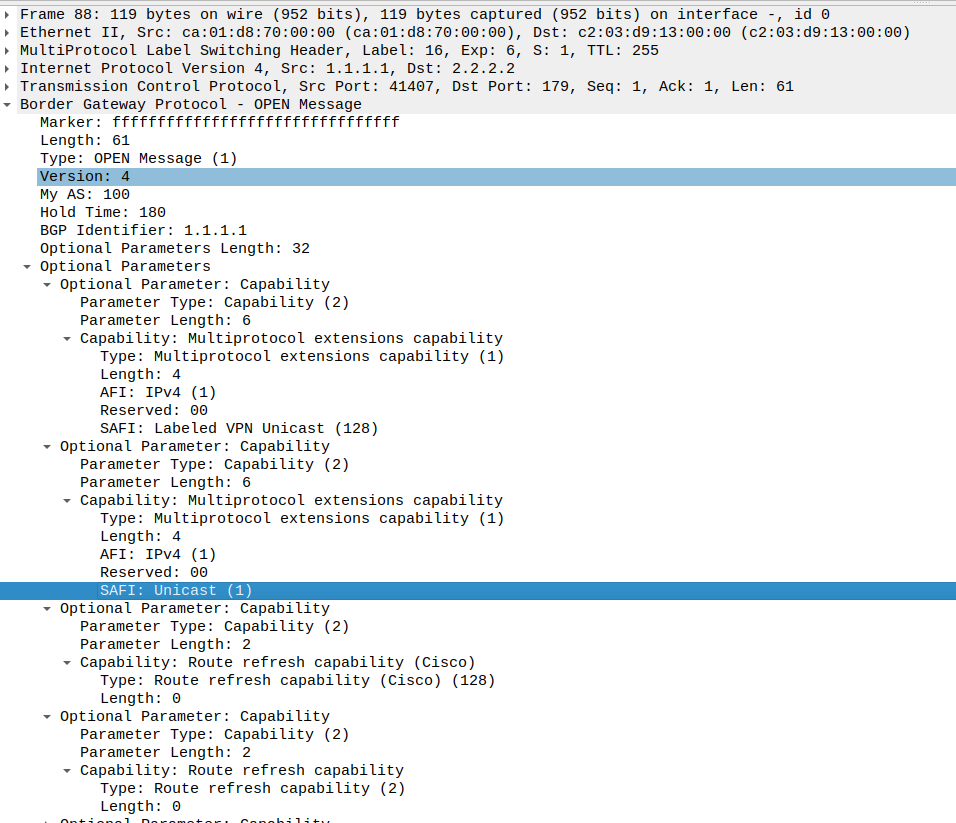
\includegraphics[width=\textwidth]{../Images/Contents BGP open msg.png}
    \caption{Content of the open message}
    \label{fig:bgp_open_pe1_content}
\end{figure}

The Open messages advertise the Multiprotocol Extensions capability (code 1) with \texttt{AFI=1} (IPv4) and \texttt{SAFI=128} (Labeled VPN Unicast). This is the critical capability that enables VPNv4 route exchange, standard BGP only supports IPv4 unicast (\texttt{SAFI=1}) and cannot carry prefixes with an attached Route Distinguisher or MPLS label. Without this capability being confirmed by both peers, no VPN routes can be signaled.

Figure~\ref{fig:bgp_update} presents the BGP Update message sent by PE2 to PE1 advertising the blue organization's remote prefix. Two path attributes are of particular relevance, as shown in Figure~\ref{fig:bgp_update_content}. The \texttt{MP\_REACH\_NLRI} attribute (type 14) confirms the negotiated address family (\texttt{AFI=1, SAFI=128}) and carries the NLRI containing three elements: the Route Distinguisher \texttt{1:1} prepended to prefix \texttt{192.168.102.0}, forming the 96-bit VPNv4 address, and VPN label \texttt{19} at the bottom of the stack. This label value directly matches the inner label observed in the previous section's Wireshark captures and PE2's MPLS forwarding table entry for \texttt{192.168.102.0/24[V]}, confirming that VPN labels are distributed via MP-BGP and not LDP. The next hop is encoded as \texttt{RD=0:0, IPv4=2.2.2.2}, identifying PE2's loopback as the reachability next hop.

\begin{figure}[H]
    \centering
    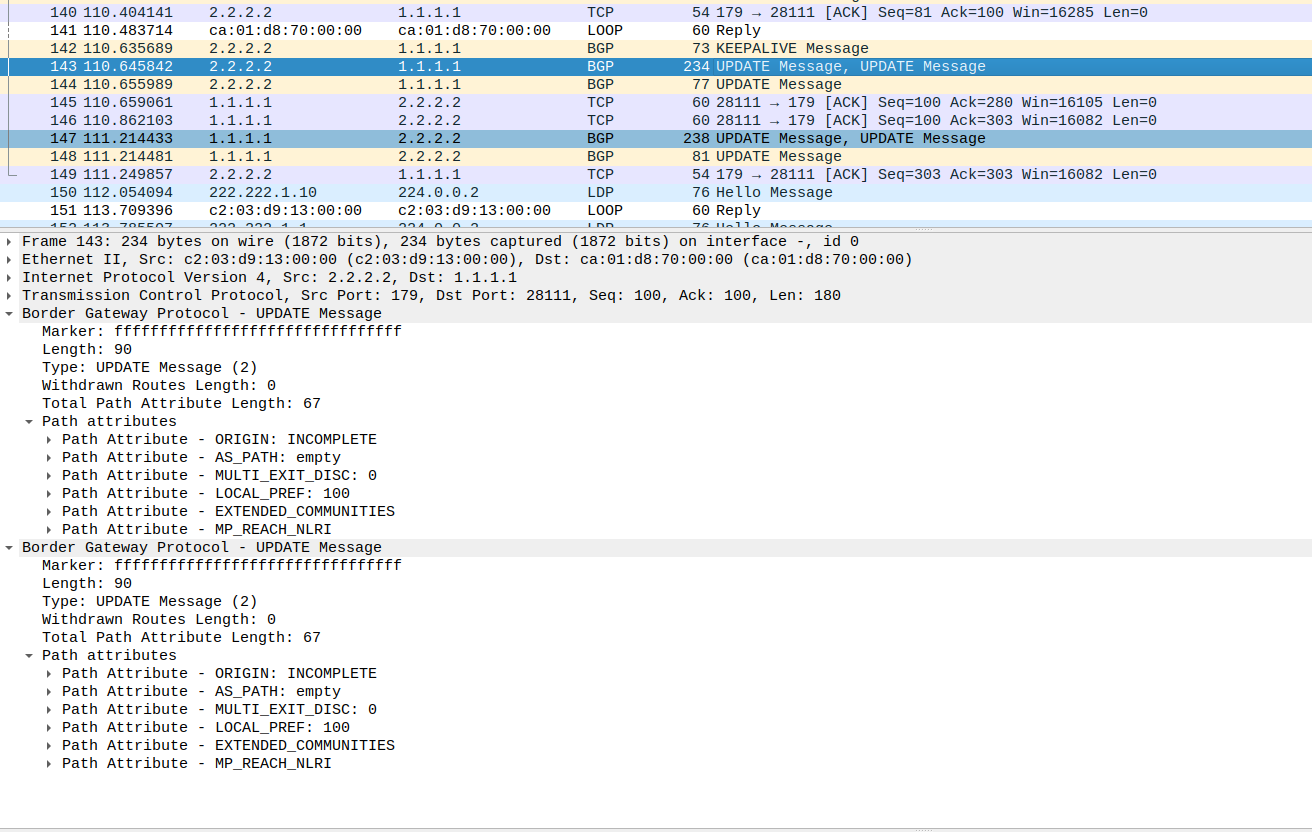
\includegraphics[width=\textwidth]{../Images/BGP update msgs.png}
    \caption{Messages exchanged}
    \label{fig:bgp_update}
\end{figure}

Two additional capabilities are also negotiated: Route Refresh (type~2), which 
allows peers to request a full re-advertisement of the BGP table without 
resetting the session, and 4-octet AS number support (type~65), which permits AS 
numbers above 65535. Both are visible in Figure~\ref{fig:bgp_open_pe1_content}.

\begin{figure}[H]
    \centering
    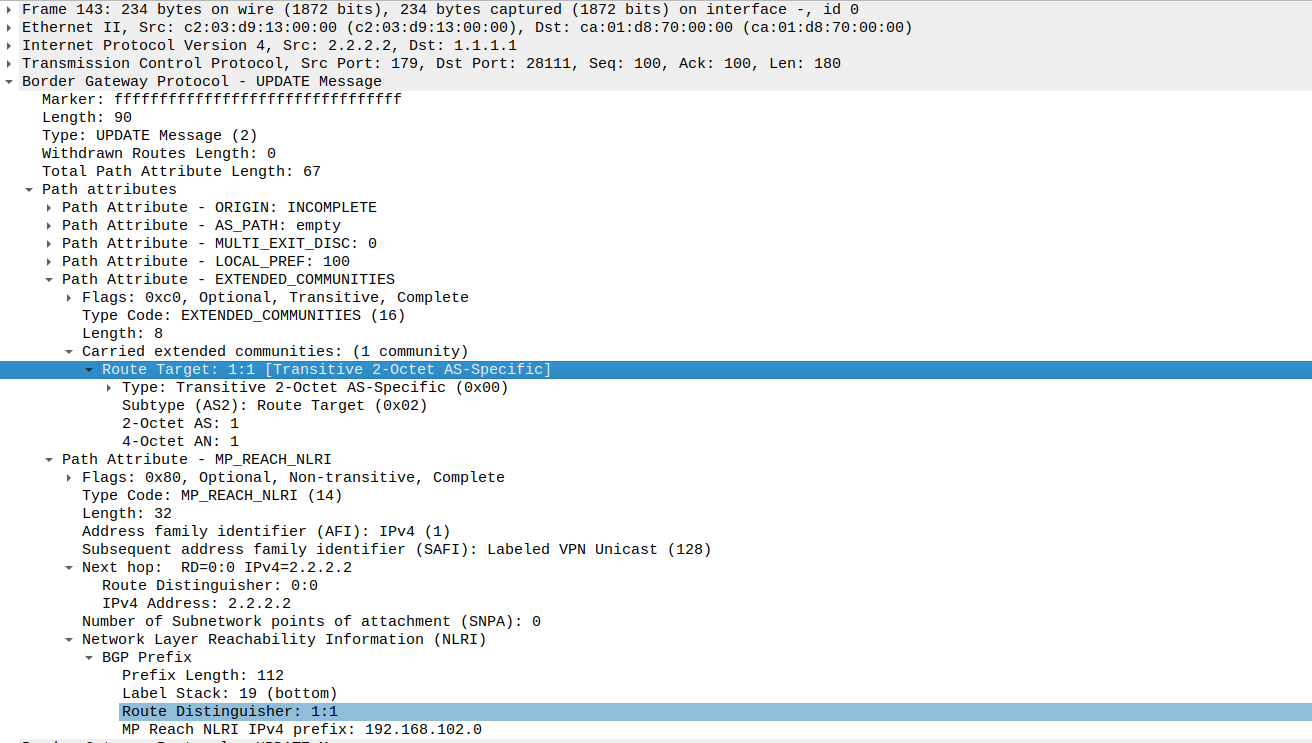
\includegraphics[width=\textwidth]{../Images/Content BGP update msg.png}
    \caption{Contents of the message}
    \label{fig:bgp_update_content}
\end{figure}

The \texttt{EXTENDED\_COMMUNITIES} attribute (type 16) carries Route Target \texttt{RT:1:1}. Upon receiving this update, PE1 imports the prefix into the blue VRF because its import policy matches \texttt{RT:1:1}, while the red VRF, configured with \texttt{route-target import 2:2}, ignores it entirely. This enforces inter-organization isolation at the control plane, complementing the data plane isolation provided by VRFs.

A VPNv4 route is an IPv4 prefix extended with a 64-bit Route Distinguisher, producing a globally unique 96-bit BGP prefix. The RD ensures overlapping customer address spaces remain distinguishable --- \texttt{1:1:192.168.102.0/24} and \texttt{2:2:192.168.102.0/24} are distinct BGP entries despite identical IPv4 portions. Crucially, the RD carries no policy semantics; routing policy is determined solely by the Route Target. Standard BGP cannot support this VPN solution because it simultaneously lacks the 64-bit RD prefix format, MPLS label encoding within the NLRI, and Extended Communities support for Route Target signaling.

\section{Connecting network namespaces with IPIP tunnel}

\subsection{Introduction}

The objective of this exercise was to establish communication between two Linux network namespaces located on different nodes using an IPIP tunnel. Two Ubuntu nodes were used: \texttt{ub1} and \texttt{ub2}. Each node contained one network namespace connected to the host through a bridge interface and a virtual Ethernet pair (veth). Communication between the namespaces was achieved by creating an IPIP tunnel between the two hosts and configuring appropriate routing rules.

A Linux network namespace is an isolated instance of the kernel's network stack, 
with its own interfaces, routing table, ARP table, and firewall rules, completely 
independent from the host and from other namespaces. It is the fundamental 
isolation primitive underlying Docker containers and other container runtimes.

\subsection{Topology}

Container \texttt{cont0} (VLAN~10, \texttt{20.10.0.10} on \texttt{ub1}) and 
\texttt{cont2} (VLAN~10, \texttt{20.10.0.11} on \texttt{ub2}) communicate using 
VLAN ID~10, as confirmed by the \texttt{802.1Q} header in 
Figure~\ref{fig:vlan10}. Containers \texttt{cont1} and \texttt{cont3} use VLAN 
ID~20, as shown in Figure~\ref{fig:vlan20}. The two VLANs are isolated at 
Layer~2 by the switch. Frames tagged with VLAN~10 are never delivered to 
interfaces associated with VLAN~20.

Figure~\ref{fig:topo_IPIP} shows the topology used.

%\begin{figure}[H]
%    \centering
%    \includegraphics[width=0.9\linewidth]{../Images/}
%    \caption{Topology}
%    \label{fig:topo_IPIP}
%\end{figure}

\subsection{Configuration of the Namespaces and Tunnel}

Two network namespaces were created, one on each node. Namespace \texttt{blue} was created on \texttt{ub1}, while namespace \texttt{red} was created on \texttt{ub2}.

\subsubsection{Namespace Configuration}

On \texttt{ub1}, the following commands were used:

\begin{verbatim}
ip netns add blue

ip link add br2 type bridge
ip link set br2 up

ip link add iblue type veth peer name ibluebr

ip link set iblue netns blue
ip link set ibluebr master br2
ip link set ibluebr up

ip -n blue addr add 10.0.2.2/24 dev iblue
ip -n blue link set iblue up
ip -n blue link set lo up

ip addr add 10.0.2.1/24 dev br2

ip netns exec blue ip route add default via 10.0.2.1
\end{verbatim}

On \texttt{ub2}, the following commands were executed:

\begin{verbatim}
ip netns add red

ip link add br1 type bridge
ip link set br1 up

ip link add ired type veth peer name iredbr

ip link set ired netns red
ip link set iredbr master br1
ip link set iredbr up

ip -n red addr add 10.0.1.2/24 dev ired
ip -n red link set ired up
ip -n red link set lo up

ip addr add 10.0.1.1/24 dev br1

ip netns exec red ip route add default via 10.0.1.1
\end{verbatim}

The bridge interfaces acted as gateways between the namespaces and the host operating systems.

\subsubsection{Physical Interface Configuration}

The physical interfaces connecting the two Ubuntu nodes were configured with IPv4 addresses:

\begin{itemize}
    \item \texttt{ub1}: \texttt{192.168.50.1/24}
    \item \texttt{ub2}: \texttt{192.168.50.2/24}
\end{itemize}

The following commands were used:

\begin{verbatim}
ip addr add 192.168.50.1/24 dev ens3
\end{verbatim}

on \texttt{ub1}, and

\begin{verbatim}
ip addr add 192.168.50.2/24 dev ens3
\end{verbatim}

on \texttt{ub2}.

\subsubsection{IPIP Tunnel Configuration}

An IPIP tunnel was created between the two hosts.

On \texttt{ub1}:

\begin{verbatim}
ip tunnel add tun0 mode ipip \
local 192.168.50.1 remote 192.168.50.2

ip addr add 192.168.100.1/30 dev tun0
ip link set tun0 up
\end{verbatim}

On \texttt{ub2}:

\begin{verbatim}
ip tunnel add tun0 mode ipip \
local 192.168.50.2 remote 192.168.50.1

ip addr add 192.168.100.2/30 dev tun0
ip link set tun0 up
\end{verbatim}

The tunnel endpoints used the physical IP addresses of the hosts, while the tunnel interfaces themselves used the network \texttt{192.168.100.0/30}.

\subsubsection{Routing and IP Forwarding}

IP forwarding was enabled on both hosts using:

\begin{verbatim}
sysctl -w net.ipv4.ip_forward=1
\end{verbatim}

Static routes were then added so that traffic destined for the remote namespace network would be forwarded through the tunnel.

On \texttt{ub1}:

\begin{verbatim}
ip route add 10.0.1.0/24 via 192.168.100.2 dev tun0
\end{verbatim}

On \texttt{ub2}:

\begin{verbatim}
ip route add 10.0.2.0/24 via 192.168.100.1 dev tun0
\end{verbatim}

With these configurations, communication between the two namespaces was successfully established through the IPIP tunnel.

\subsection{Verification of Connectivity}

After configuring the namespaces, bridge interfaces, tunnel interfaces and routing tables, connectivity between the two namespaces was tested using ICMP echo requests.

The following command was executed from the namespace located on \texttt{ub1}:

\begin{verbatim}
ip netns exec blue ping 10.0.1.2
\end{verbatim}

The ping was successful, confirming that packets were correctly routed through the IPIP tunnel between the two hosts.

Figure~\ref{fig:ping} shows the successful communication between the namespaces.

\begin{figure}[H]
    \centering
    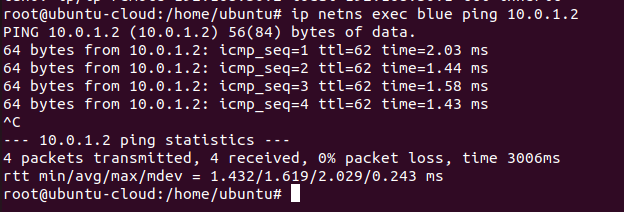
\includegraphics[width=0.9\linewidth]{../Images/ping from ub1 to ub2.png}
    \caption{Successful ping between namespaces}
    \label{fig:ping}
\end{figure}

The routing tables were also verified to ensure that traffic destined for the remote namespace network was forwarded through the tunnel interface \texttt{tun0}.

Figure~\ref{fig:routes} shows the routing table and network interfaces configured on \texttt{ub2}.

\begin{figure}[H]
    \centering
    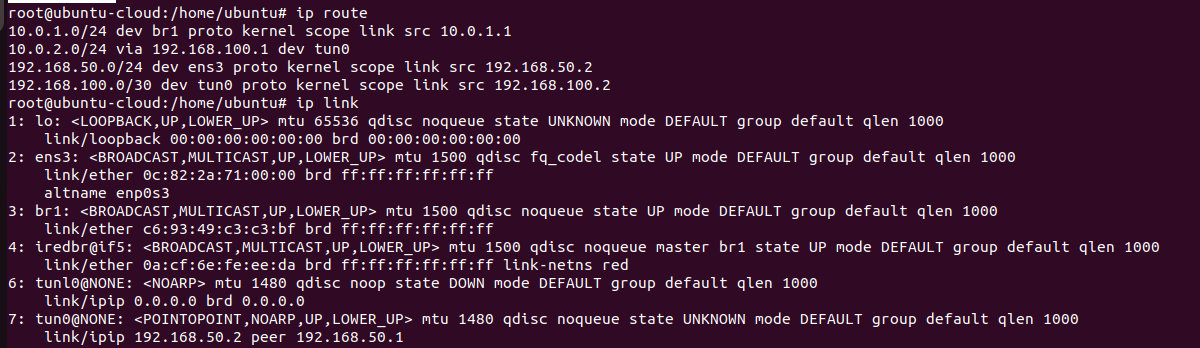
\includegraphics[width=0.9\linewidth]{../Images/ip route & ip link ub2.png}
    \caption{Routing table and interfaces on ub2}
    \label{fig:routes}
\end{figure}

\subsection{Verification of IPIP Encapsulation}

To verify that the communication between namespaces was effectively using IPIP tunneling, packets were captured on the physical interface connecting the two hosts using Wireshark.

The capture revealed that the packets contained two IP headers:

\begin{itemize}
    \item an outer IP header containing the physical addresses of the hosts (\texttt{192.168.50.1} and \texttt{192.168.50.2});
    \item an inner IP header containing the original namespace communication addresses (\texttt{10.0.2.2} and \texttt{10.0.1.2}).
\end{itemize}

This confirms that the original packets were encapsulated inside another IP packet before being transmitted through the physical network.

Figure~\ref{fig:wireshark} shows the Wireshark capture illustrating the double IP header generated by the IPIP tunnel.

\begin{figure}[H]
    \centering
    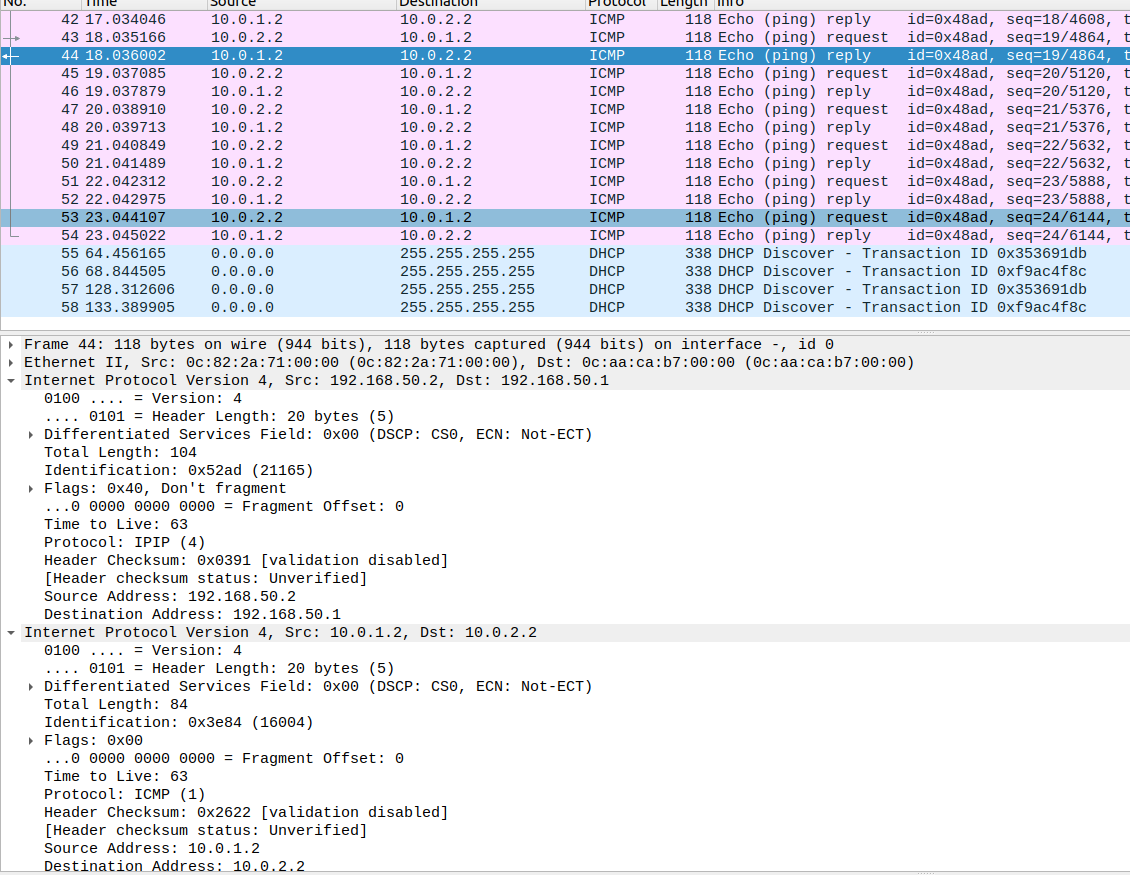
\includegraphics[width=0.95\linewidth]{../Images/IPIP tunnel ping.png}
    \caption{Wireshark capture showing IPIP encapsulation}
    \label{fig:wireshark}
\end{figure}

\subsection{Tunnel Verification}

The tunnel configuration was verified using the command:

\begin{verbatim}
ip tunnel show
\end{verbatim}

The output confirmed that the tunnel interface \texttt{tun0} was active and correctly configured with the local and remote endpoints.

Figure~\ref{fig:tunnel} shows the tunnel configuration on \texttt{ub2}.

\begin{figure}[H]
    \centering
    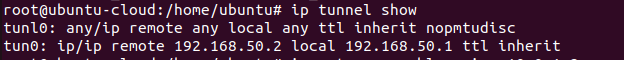
\includegraphics[width=0.85\linewidth]{../Images/tunnel show in ub2.png}
    \caption{IPIP tunnel configuration}
    \label{fig:tunnel}
\end{figure}

\section{Macvlan Networks with VLAN Isolation}

\subsection{Introduction}

The objective of this exercise was to configure isolated Docker macvlan networks using IEEE 802.1Q VLAN tagging. Two Ubuntu nodes, \texttt{ub1} and \texttt{ub2}, were connected through a Layer 2 Ethernet switch and configured with VLAN subinterfaces. Docker macvlan networks were then attached to these VLAN interfaces, allowing containers connected to the same VLAN to communicate while isolating traffic between different VLANs.

Two VLANs were configured:

\begin{itemize}
    \item VLAN 10 using subnet \texttt{20.10.0.0/24};
    \item VLAN 20 using subnet \texttt{20.20.0.0/24}.
\end{itemize}

Each Ubuntu node hosted one container connected to VLAN 10 and one container connected to VLAN 20. This allowed communication between containers attached to the same VLAN across different nodes, while preventing communication between containers attached to different VLANs.

The experiment demonstrates how Docker macvlan networks can be combined with IEEE 802.1Q VLAN tagging to provide Layer 2 isolation between groups of containers distributed across multiple hosts.

\subsection{VLAN Interface Configuration}

IEEE 802.1Q support was enabled on both Ubuntu nodes using the Linux \texttt{8021q} kernel module.

The following commands were executed on both \texttt{ub1} and \texttt{ub2}:

\begin{verbatim}
modprobe 8021q

ip link add link ens3 name ens3.10 type vlan id 10
ip link add link ens3 name ens3.20 type vlan id 20

ip link set ens3.10 up
ip link set ens3.20 up
\end{verbatim}

These commands created two VLAN subinterfaces associated with the physical interface \texttt{ens3}. Interface \texttt{ens3.10} was associated with VLAN ID 10, while interface \texttt{ens3.20} was associated with VLAN ID 20.

No IP addresses were assigned to the VLAN subinterfaces, since they were used exclusively as Layer 2 parent interfaces for the Docker macvlan networks.

Figure~\ref{fig:vlaninterfaces} shows the interfaces configured on \texttt{ub1}.

\begin{figure}[H]
    \centering
    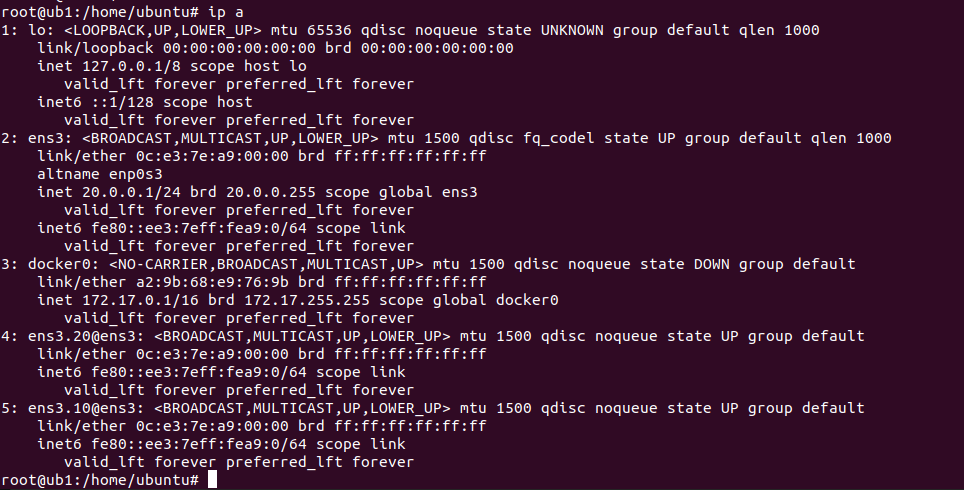
\includegraphics[width=0.9\linewidth]{../Images/ip a ub1 cont VLAN.png}
    \caption{Physical and VLAN interfaces configured on ub1}
    \label{fig:vlaninterfaces}
\end{figure}

\subsection{Macvlan Network Configuration}

Two Docker macvlan networks were created on each node.

The following commands were executed:

\begin{verbatim}
docker network create -d macvlan \
--subnet=20.10.0.0/24 \
-o parent=ens3.10 mynet10

docker network create -d macvlan \
--subnet=20.20.0.0/24 \
-o parent=ens3.20 mynet20
\end{verbatim}

The network \texttt{mynet10} was attached to VLAN interface \texttt{ens3.10}, while network \texttt{mynet20} was attached to VLAN interface \texttt{ens3.20}.

Figure~\ref{fig:dockerNetworks} shows the Docker networks configured on \texttt{ub1}.

\begin{figure}[H]
    \centering
    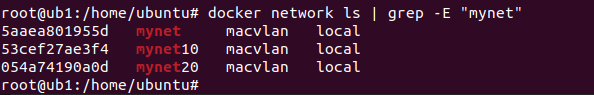
\includegraphics[width=0.8\linewidth]{../Images/docker network ls ub1 cont VLAN.png}
    \caption{Docker macvlan networks configured on ub1}
    \label{fig:dockerNetworks}
\end{figure}

The detailed configuration of network \texttt{mynet10} was also verified using Docker inspection commands.

Figure~\ref{fig:inspectNetwork} shows the configuration of \texttt{mynet10}.

\begin{figure}[H]
    \centering
    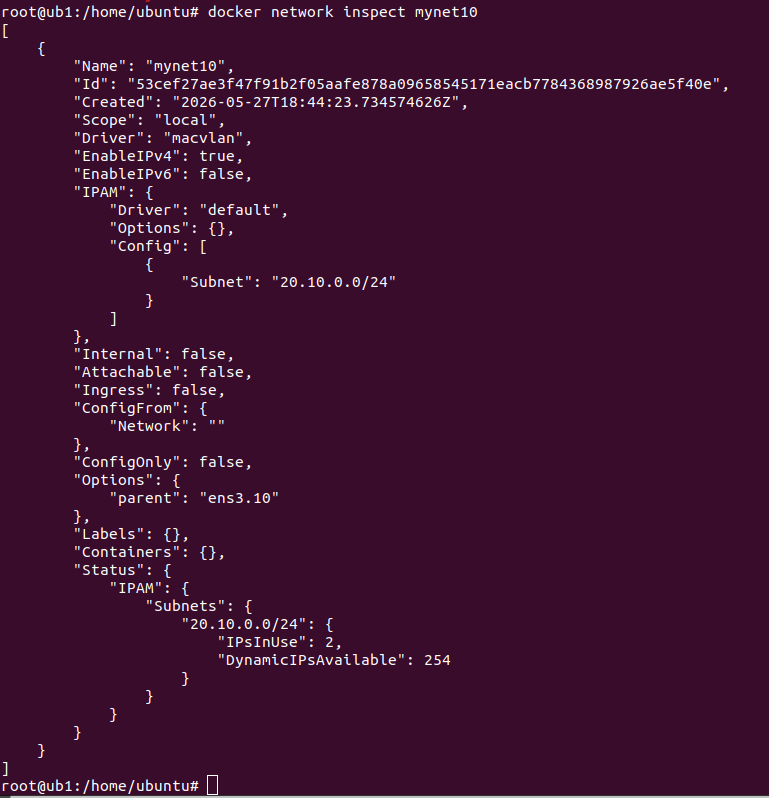
\includegraphics[width=0.95\linewidth]{../Images/inspect mynet10 ub1 cont VLAN.png}
    \caption{Inspection of Docker macvlan network mynet10}
    \label{fig:inspectNetwork}
\end{figure}

\subsection{Container Deployment}

Containers were then attached to the corresponding VLAN networks.

On \texttt{ub1}, the following containers were created:

\begin{verbatim}
docker run --privileged --net=mynet10 \
--ip=20.10.0.10 --name=cont0 -itd alpine /bin/sh

docker run --privileged --net=mynet20 \
--ip=20.20.0.10 --name=cont1 -itd alpine /bin/sh
\end{verbatim}

On \texttt{ub2}, the following containers were created:

\begin{verbatim}
docker run --privileged --net=mynet10 \
--ip=20.10.0.11 --name=cont2 -itd alpine /bin/sh

docker run --privileged --net=mynet20 \
--ip=20.20.0.11 --name=cont3 -itd alpine /bin/sh
\end{verbatim}

Each node therefore hosted one container in VLAN 10 and one container in VLAN 20.

Figure~\ref{fig:dockerps} shows the running containers on \texttt{ub1}.

\begin{figure}[H]
    \centering
    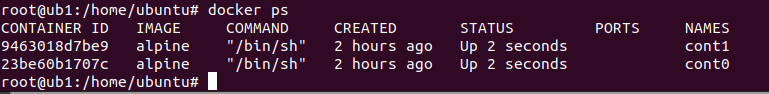
\includegraphics[width=0.85\linewidth]{../Images/docker ps ub1 cont VLAN.png}
    \caption{Running containers on ub1}
    \label{fig:dockerps}
\end{figure}

\subsection{Verification of Connectivity and Isolation}

Connectivity tests were performed using ICMP echo requests between containers attached to the same VLAN.

The following command was executed on \texttt{ub1}:

\begin{verbatim}
docker exec cont0 ping 20.10.0.11
\end{verbatim}

The ping was successful, confirming communication between containers connected to VLAN 10 across different nodes.

Similarly, communication between containers connected to VLAN 20 was verified using:

\begin{verbatim}
docker exec cont1 ping 20.20.0.11
\end{verbatim}

Additional tests were then performed between containers attached to different VLANs. These communication attempts failed, confirming that VLAN isolation was correctly enforced.

Communication between mynet10 and mynet20 was also tested.

To test that the communication fails the following command was executed on \texttt{ub1}:

\begin{verbatim}
docker exec cont0 ping 20.20.0.11
\end{verbatim}

and:

\begin{verbatim}
docker exec cont1 ping 20.10.0.11
\end{verbatim}

Figure~\ref{fig:successfulPing} shows both successful communication between containers attached to the same VLAN and failed communication attempts between containers attached to different VLANs.

\begin{figure}[H]
    \centering
    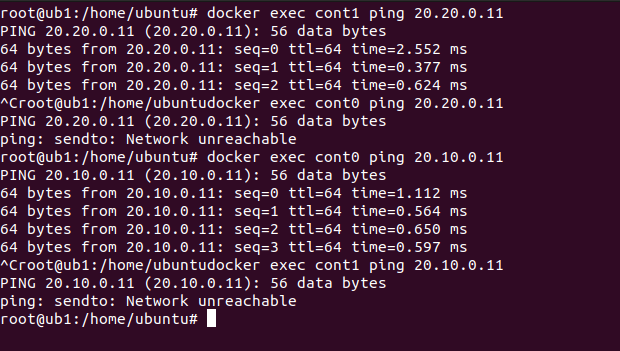
\includegraphics[width=0.95\linewidth]{../Images/pings between containers VLAN.png}
    \caption{Connectivity tests between containers in the same and different VLANs}
    \label{fig:successfulPing}
\end{figure}

\subsection{Traffic Analysis}

Packet captures were performed using Wireshark on the GNS3 links connecting the Ubuntu nodes to the Ethernet switch.

The captures revealed Ethernet frames containing IEEE 802.1Q headers with VLAN identifiers 10 and 20, confirming that VLAN tagging was correctly applied to the transmitted traffic.

Containers attached to VLAN 10 exchanged packets containing VLAN ID 10, while containers attached to VLAN 20 exchanged packets containing VLAN ID 20.

Figures~\ref{fig:vlan10} and~\ref{fig:vlan20} show captured frames containing IEEE 802.1Q VLAN headers for VLANs 10 and 20, respectively.

\begin{figure}[H]
    \centering
    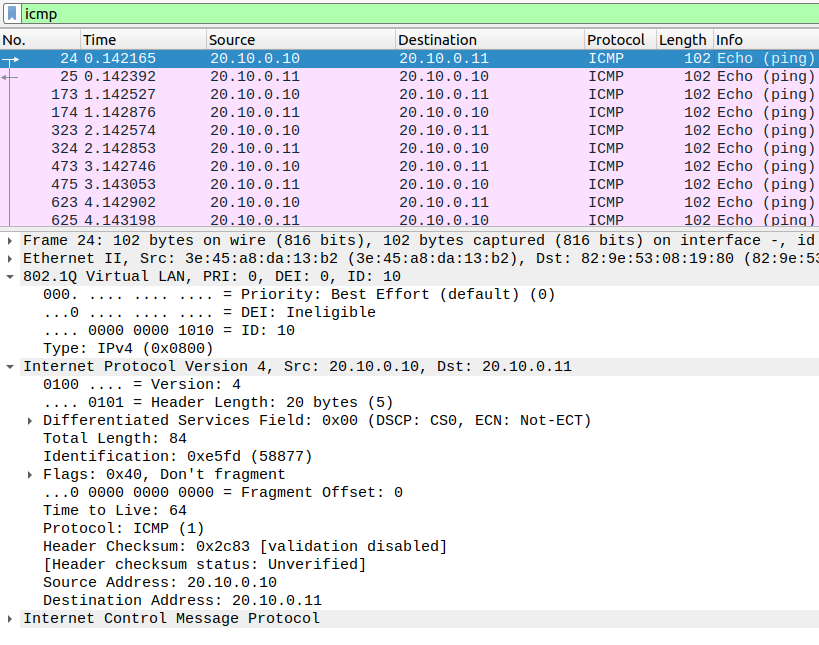
\includegraphics[width=0.95\linewidth]{../Images/VLAN 802.1Q id 10.png}
    \caption{Wireshark capture showing IEEE 802.1Q VLAN tagging with VLAN ID 10}
    \label{fig:vlan10}
\end{figure}

\begin{figure}[H]
    \centering
    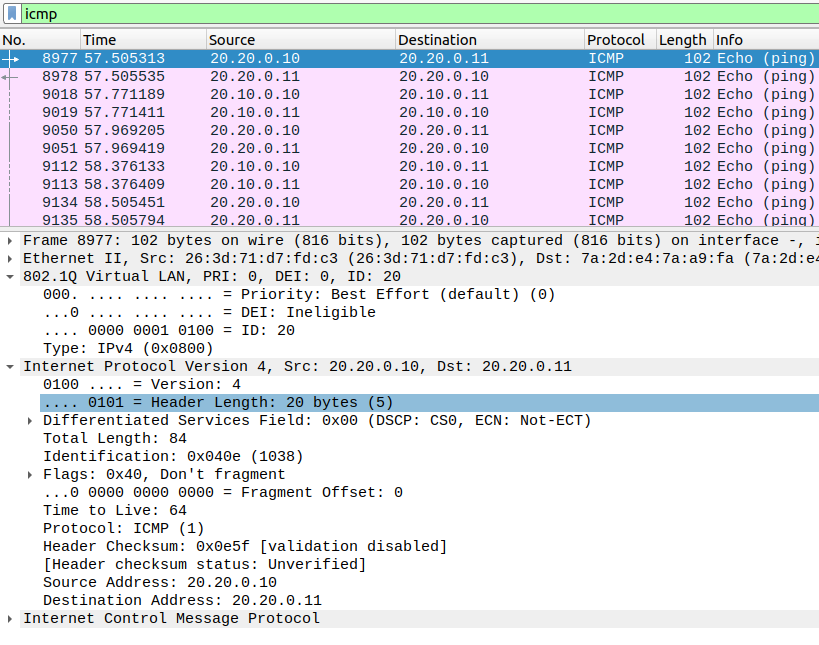
\includegraphics[width=0.95\linewidth]{../Images/VLAN 802.1Q id 20.png}
    \caption{Wireshark capture showing IEEE 802.1Q VLAN tagging with VLAN ID 20}
    \label{fig:vlan20}
\end{figure}

The source and destination MAC addresses observed in the captured frames corresponded directly to the MAC addresses assigned to the communicating containers. The physical interfaces of the Ubuntu hosts acted as transport interfaces responsible for transmitting VLAN-tagged Ethernet frames between the two nodes through the Ethernet switch.

\subsection{Discussion and Limitations}

The experiment demonstrated that Docker macvlan networks can be combined with IEEE 802.1Q VLAN tagging to provide Layer 2 isolation between containers distributed across multiple hosts.

Containers attached to the same VLAN were able to communicate directly through the Ethernet switch, while communication between different VLANs was blocked.

One limitation of macvlan networks is that the host system cannot directly communicate with containers attached to the macvlan interface unless additional routing or bridge configurations are introduced. Another limitation is that troubleshooting and packet captures may be more complex because traffic generated by macvlan interfaces is not always visible through standard host interface captures depending on the Linux networking path used internally by Docker and the kernel.

The physical interfaces of the Ubuntu nodes acted as transport media for VLAN-tagged Ethernet frames exchanged between containers located on different hosts, while the VLAN subinterfaces provided logical Layer 2 separation between the different macvlan networks.

\section{Linux VXLAN with Multicast Routing}
 
\subsection{Introduction}
 
The objective of this exercise was to create two overlay networks using VXLAN technology combined with IP multicast routing. All three Ubuntu nodes from the network scenario were used: \texttt{ub1} and \texttt{ub2}, connected to router \texttt{R1} via \texttt{Switch1} on the \texttt{20.0.0.0/24} subnet, and \texttt{ub3}, connected directly to \texttt{R1} on the \texttt{21.0.0.0/24} subnet.
 
Two overlay networks were configured:
 
\begin{itemize}
    \item \texttt{bluenet}, using subnet \texttt{10.0.0.0/24} and VXLAN Network Identifier (VNI) 33, associated with multicast group \texttt{239.1.1.3};
    \item \texttt{rednet}, using subnet \texttt{11.0.0.0/24} and VNI 66, associated with multicast group \texttt{239.1.1.6}.
\end{itemize}
 
A total of ten containers were deployed across the three nodes. The distribution of containers per node and network is shown in Table~\ref{tab:containers}.
 
\begin{table}[H]
\centering
\begin{tabular}{|c|c|c|}
\hline
 & \textbf{bluenet} & \textbf{rednet} \\
\hline
\texttt{ub1} & b1: 10.0.0.1, b2: 10.0.0.2 & r1: 11.0.0.1, r2: 11.0.0.2 \\
\hline
\texttt{ub2} & b3: 10.0.0.3, b4: 10.0.0.4 & r3: 11.0.0.3, r4: 11.0.0.4 \\
\hline
\texttt{ub3} & b5: 10.0.0.5, b6: 10.0.0.6 & --- \\
\hline
\end{tabular}
\caption{Distribution of containers per node and network}
\label{tab:containers}
\end{table}
 
Node \texttt{ub3} was only connected to \texttt{bluenet}, as it does not participate in \texttt{rednet}.
 
\subsection{VXLAN Interface Configuration}
 
The configuration procedure at each node consisted of five steps: creating the VXLAN interfaces, activating them, assigning IP addresses, creating Docker macvlan networks, and deploying containers.
 
On \texttt{ub1}, two VXLAN interfaces were created and configured as follows:
 
\begin{verbatim}
ip link add blue type vxlan id 33 group 239.1.1.3 ttl 5 dev ens3 dstport 4789
ip link add red  type vxlan id 66 group 239.1.1.6 ttl 5 dev ens3 dstport 4789
 
ip link set blue up
ip link set red  up
 
ip addr add 10.0.0.101/24 dev blue
ip addr add 11.0.0.101/24 dev red
\end{verbatim}
 
Each VXLAN interface was bound to the physical interface \texttt{ens3} and configured to use UDP destination port 4789, the IANA-assigned port for VXLAN. The \texttt{group} parameter associates each interface with a distinct IP multicast group, so that broadcast and unknown unicast traffic within each overlay network is distributed via multicast rather than flooding all endpoints. The TTL was set to 5 to limit multicast propagation scope.
 
The IP addresses assigned to the VXLAN interfaces serve as the gateway addresses for the Docker macvlan networks created on that node. Each node was assigned a distinct gateway: \texttt{.101} on \texttt{ub1}, \texttt{.102} on \texttt{ub2}, and \texttt{.103} on \texttt{ub3}.
 
The same procedure was repeated on \texttt{ub2} and \texttt{ub3}, with the respective addresses and, in the case of \texttt{ub3}, only the \texttt{blue} interface being created.
 
Figure~\ref{fig:vxlan_interfaces} shows the VXLAN interfaces configured on \texttt{ub1}.
 
\begin{figure}[H]
\centering
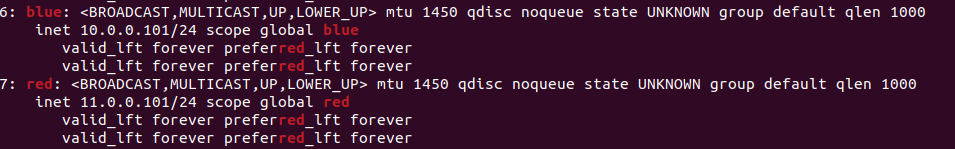
\includegraphics[width=0.9\linewidth]{../Images/vxlan interfaces ub1.png}
\caption{VXLAN interfaces configured on ub1}
\label{fig:vxlan_interfaces}
\end{figure}
 
\subsection{Docker Network and Container Deployment}
 
Two Docker macvlan networks were created on \texttt{ub1}, each attached to the corresponding VXLAN interface:
 
\begin{verbatim}
docker network create -d macvlan \
  --subnet=10.0.0.0/24 --gateway=10.0.0.101 \
  -o parent=blue bluenet
 
docker network create -d macvlan \
  --subnet=11.0.0.0/24 --gateway=11.0.0.101 \
  -o parent=red rednet
\end{verbatim}
 
Containers were then created and attached to the appropriate networks:
 
\begin{verbatim}
docker run --privileged --net=bluenet --name=b1 --ip=10.0.0.1 -itd alpine /bin/sh
docker run --privileged --net=bluenet --name=b2 --ip=10.0.0.2 -itd alpine /bin/sh
docker run --privileged --net=rednet  --name=r1 --ip=11.0.0.1 -itd alpine /bin/sh
docker run --privileged --net=rednet  --name=r2 --ip=11.0.0.2 -itd alpine /bin/sh
\end{verbatim}
 
The same procedure was followed on \texttt{ub2} and \texttt{ub3}, adjusting container names, IP addresses, and gateway addresses accordingly. On \texttt{ub3}, only the \texttt{bluenet} network and containers \texttt{b5} and \texttt{b6} were created.
 
Figure~\ref{fig:docker_networks} shows the Docker networks created on \texttt{ub1}, and Figure~\ref{fig:docker_containers} shows all running containers.
 
\begin{figure}[H]
\centering
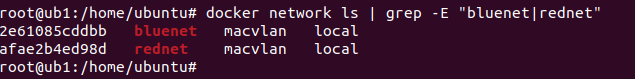
\includegraphics[width=0.8\linewidth]{../Images/docker network ls ub1.png}
\caption{Docker macvlan networks on ub1}
\label{fig:docker_networks}
\end{figure}
 
\begin{figure}[H]
\centering
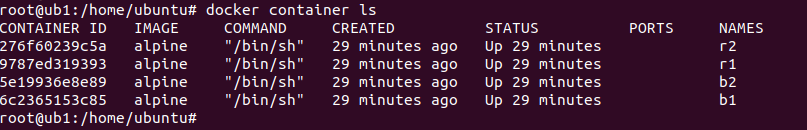
\includegraphics[width=0.8\linewidth]{../Images/docker container ls ub1.png}
\caption{Running containers on ub1}
\label{fig:docker_containers}
\end{figure}
 
\subsection{Multicast Routing Configuration}
 
Protocol Independent Multicast in Dense Mode (PIM-DM) was enabled on router \texttt{R1} to support the distribution of multicast traffic between the two network segments. The following configuration was applied:
 
\begin{verbatim}
ip multicast-routing
 
interface f0/0
 ip pim dense-mode
 
interface f0/1
 ip pim dense-mode
\end{verbatim}
 
PIM Dense Mode was chosen as it floods multicast traffic on all interfaces and subsequently prunes branches where no listeners are present. Both interfaces were configured since \texttt{f0/0} connects to the segment containing \texttt{ub1} and \texttt{ub2}, while \texttt{f0/1} connects to the segment containing \texttt{ub3}.
 
\subsection{Connectivity Verification}
 
After completing the configuration on all nodes, connectivity between containers of the same overlay network was verified using ICMP echo requests.
 
The following tests were performed from \texttt{ub1}:
 
\begin{verbatim}
docker exec b1 ping -c 4 10.0.0.2   # b1 -> b2, same node
docker exec b1 ping -c 4 10.0.0.3   # b1 -> b3, ub1 -> ub2
docker exec b2 ping -c 4 10.0.0.6   # b2 -> b6, ub1 -> ub3
docker exec r1 ping -c 4 11.0.0.3   # r1 -> r3, rednet ub1 -> ub2
\end{verbatim}
 
All pings were successful, confirming that the overlay networks were correctly established across all three nodes and that multicast routing at \texttt{R1} was forwarding traffic between the two physical segments.
 
Figure~\ref{fig:ping_results} shows the results of the connectivity tests.
 
\begin{figure}[H]
\centering
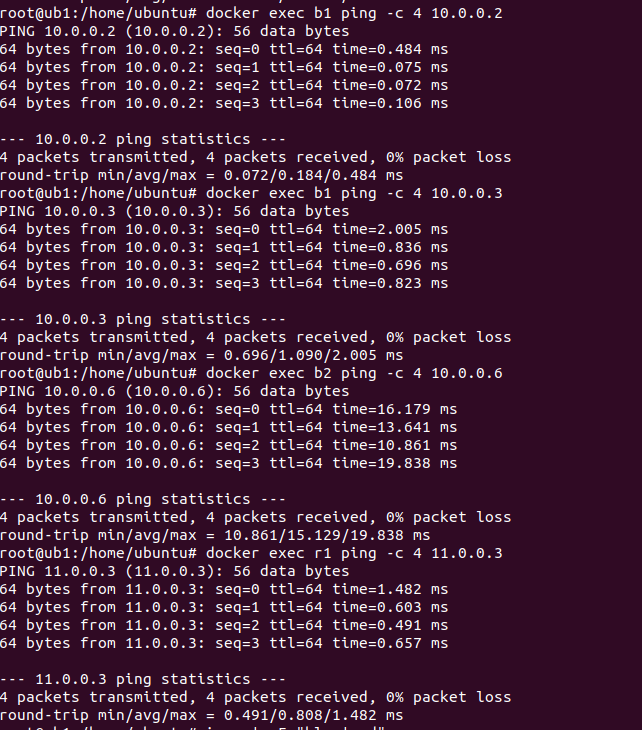
\includegraphics[width=0.9\linewidth]{../Images/ping results ub1 VXLAN.png}
\caption{Successful ping tests between containers across nodes}
\label{fig:ping_results}
\end{figure}
 
\subsection{IGMP Analysis}
 
Wireshark captures performed on the \texttt{ens3} interfaces of each node revealed IGMP Membership Report messages being transmitted when the VXLAN interfaces were brought up. These messages inform \texttt{R1} that a node wishes to receive traffic destined for a given multicast group.
 
Nodes \texttt{ub1} and \texttt{ub2} transmitted membership reports for both multicast groups \texttt{239.1.1.3} and \texttt{239.1.1.6}, corresponding to \texttt{bluenet} and \texttt{rednet} respectively. Node \texttt{ub3}, having only a \texttt{blue} interface, transmitted a membership report only for group \texttt{239.1.1.3}.
 
This was confirmed at \texttt{R1} using the command \texttt{show ip igmp groups}, the output of which is shown in Figure~\ref{fig:igmp_groups}.
 
\begin{figure}[H]
\centering
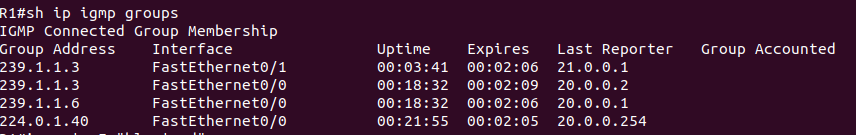
\includegraphics[width=0.85\linewidth]{../Images/igmp groups r1.png}
\caption{IGMP group membership table at R1}
\label{fig:igmp_groups}
\end{figure}
 
Group \texttt{239.1.1.3} appeared on both \texttt{FastEthernet0/0} and \texttt{FastEthernet0/1}, reflecting that all three nodes joined \texttt{bluenet}. Group \texttt{239.1.1.6} appeared only on \texttt{FastEthernet0/0}, confirming that \texttt{ub3} did not join \texttt{rednet}.
 
Figure~\ref{fig:igmp_capture} shows a Wireshark capture of an IGMP Membership Report transmitted by \texttt{ub3}.
 
\begin{figure}[H]
\centering
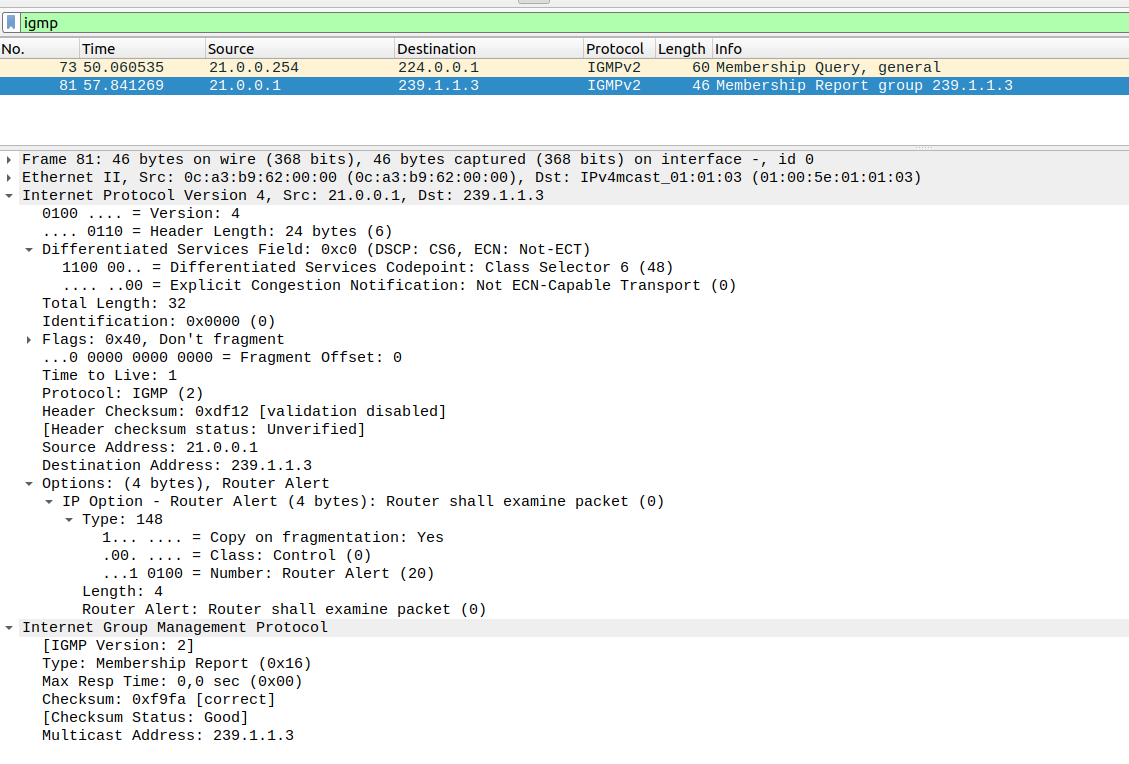
\includegraphics[width=0.95\linewidth]{../Images/membership report multicast R1-ub3.png}
\caption{IGMP Membership Report captured on ub3}
\label{fig:igmp_capture}
\end{figure}
 
\subsection{ARP and ICMP Encapsulation Analysis}
 
To trigger ARP traffic for analysis, the ARP cache of container \texttt{b1} was cleared before initiating a ping to \texttt{b6} on \texttt{ub3}:
 
\begin{verbatim}
docker exec b1 /bin/sh -c "arp -d 10.0.0.6; ping -c 4 10.0.0.6"
\end{verbatim}
 
Wireshark captures were performed on the \texttt{ens3} interface of \texttt{ub1} to observe the full encapsulation of the resulting packets.
 
\subsubsection{Packet Encapsulation}
 
All traffic between containers located on different nodes was encapsulated using the VXLAN protocol. Each packet consisted of two layers of IP addressing: an \textit{inner} IP header carrying the original container-to-container traffic, and an \textit{outer} IP header used for routing across the physical underlay network.
 
The inner IP header contained the container source and destination addresses (e.g. \texttt{10.0.0.1} $\rightarrow$ \texttt{10.0.0.6}), while the outer IP header contained the physical node addresses (e.g. \texttt{20.0.0.1} $\rightarrow$ \texttt{21.0.0.1}). The inner frame was encapsulated in a UDP datagram with destination port 4789, preceded by an 8-byte VXLAN header containing the VNI field.
 
Figure~\ref{fig:icmp_encap} shows the full encapsulation of a captured ICMP echo request.
 
\begin{figure}[H]
\centering
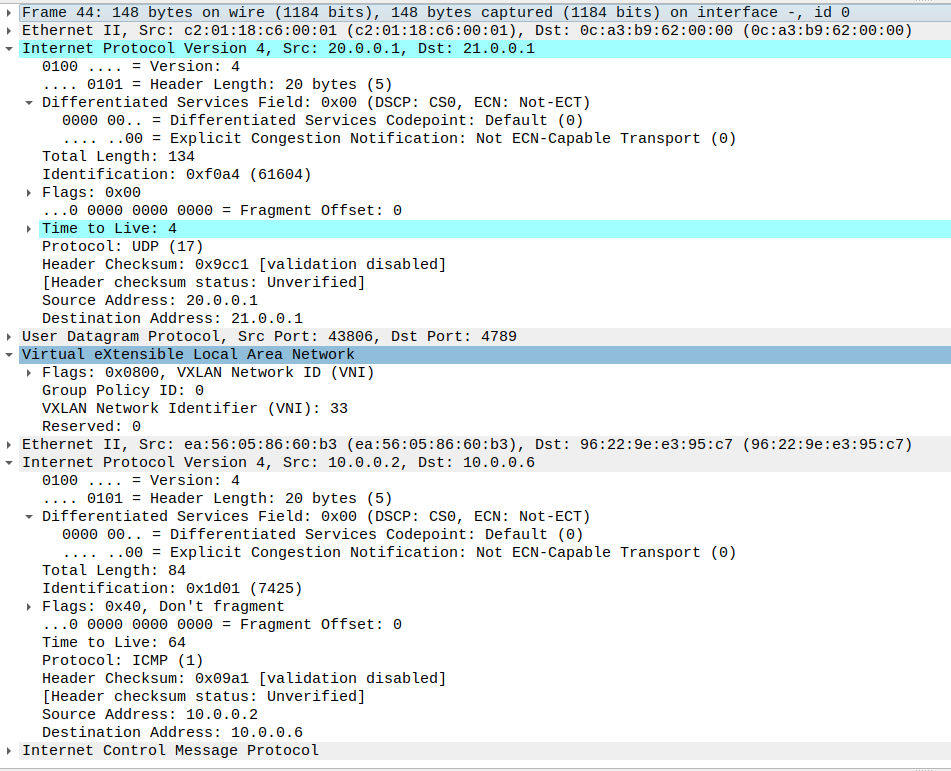
\includegraphics[width=0.95\linewidth]{../Images/icmp encapsulation VXLAN.png}
\caption{VXLAN encapsulation of an ICMP echo request between b2 and b6, captured on the R1–ub3 link (outer IP TTL decremented to 4 by R1)}
\label{fig:icmp_encap}
\end{figure}
 
\subsubsection{ARP Request and Reply}
 
ARP Request packets were sent with a multicast outer IP destination address corresponding to the VXLAN group of the overlay network (\texttt{239.1.1.3} for \texttt{bluenet}). This ensures that all nodes participating in the overlay receive the broadcast ARP Request, since VXLAN has no mechanism to natively broadcast at the underlay level. ARP Replies, being unicast, were encapsulated with the specific physical IP of the responding node as the outer destination.
 
The multicast destination address used in ARP Requests differs between networks: \texttt{bluenet} uses \texttt{239.1.1.3} while \texttt{rednet} uses \texttt{239.1.1.6}, as each overlay is associated with a distinct multicast group.
 
Figure~\ref{fig:arp_request} shows a captured ARP Request and Figure~\ref{fig:arp_reply} shows the corresponding ARP Reply.
 
\begin{figure}[H]
\centering
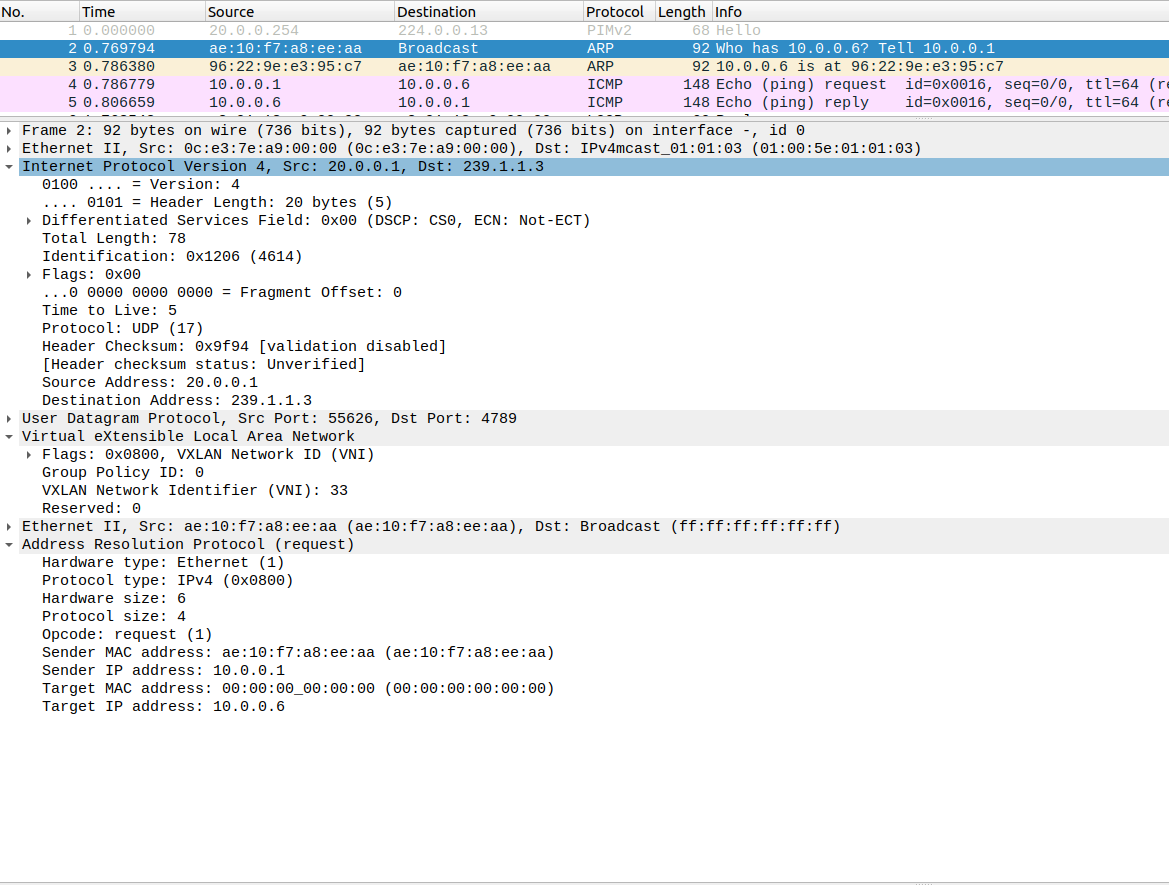
\includegraphics[width=0.95\linewidth]{../Images/arp request VXLAN.png}
\caption{ARP Request encapsulated in VXLAN with multicast outer destination}
\label{fig:arp_request}
\end{figure}
 
\begin{figure}[H]
\centering
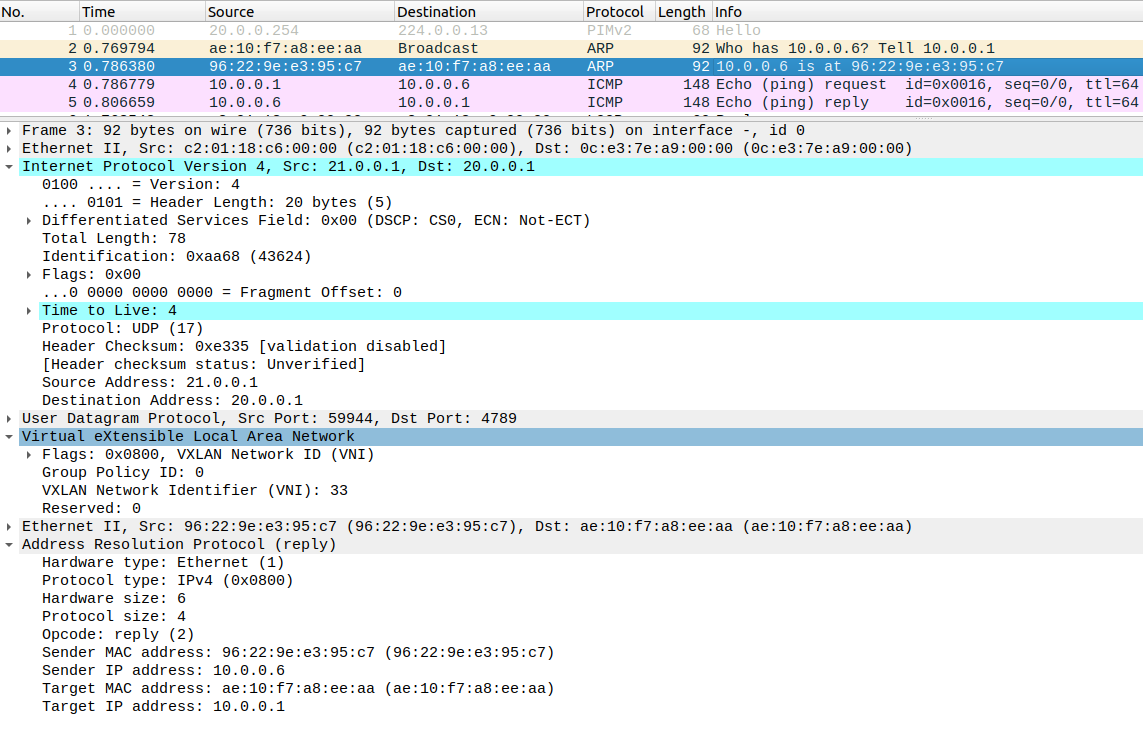
\includegraphics[width=0.95\linewidth]{../Images/arp reply VXLAN.png}
\caption{ARP Reply encapsulated in VXLAN with unicast outer destination}
\label{fig:arp_reply}
\end{figure}
 
\subsubsection{ARP Cache}
 
After the ping completed, the ARP cache of container \texttt{b1} was inspected using \texttt{arp -n}. The cache contained an entry mapping \texttt{10.0.0.6} to the MAC address of container \texttt{b6}'s network interface, matching exactly the inner Ethernet source address observed in the ARP Reply capture. This confirms that the ARP mechanism operates entirely at the overlay level, with containers unaware of the underlying VXLAN encapsulation.
 
Figure~\ref{fig:arp_cache} shows the ARP cache of container \texttt{b1} after the ping.
 
\begin{figure}[H]
\centering
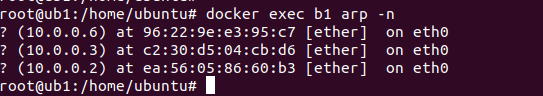
\includegraphics[width=0.75\linewidth]{../Images/arp cache in ub1 b1.png}
\caption{ARP cache of container b1 after pinging b6}
\label{fig:arp_cache}
\end{figure}
 
\subsubsection{VNI Field}
 
The VXLAN header carries a 24-bit VNI field that identifies the overlay network to which the encapsulated frame belongs. In this exercise, VNI 33 was used for \texttt{bluenet} and VNI 66 for \texttt{rednet}. Upon receiving a VXLAN packet, the destination node uses the VNI to demultiplex the inner frame into the correct overlay network, in the same way that a VLAN tag identifies a broadcast domain on a trunk link. This allows multiple isolated overlay networks to coexist on the same physical infrastructure and share the same UDP port without frames leaking between networks.

%------------------------------------------------------------
\subsection{Comparison with AI Tool Explanation}
\label{sec:vxlan_ai}
%------------------------------------------------------------

The AI tool was asked to explain the role of IGMP and multicast routing in this 
setup, and to predict how ARP and ICMP packets would be encapsulated across nodes.

The AI correctly described the general role of IGMP: each node signals membership 
in the multicast group associated with its VXLAN interface, so that ARP broadcasts 
--- which have no native VXLAN broadcast mechanism --- can be distributed to all 
VTEP endpoints in the overlay. It also correctly predicted the double-encapsulation 
structure: inner Ethernet/IP carrying container addresses, outer UDP/IP carrying 
physical node addresses, with destination port 4789.

Two discrepancies emerged from the experimental results. First, the AI stated that 
ARP Replies would be sent to the multicast group address, like ARP Requests. The 
captures in Figures~\ref{fig:arp_request} and~\ref{fig:arp_reply} show otherwise: 
ARP Replies use a unicast outer destination --- the physical IP of the node hosting 
the requesting container --- not the multicast group address. This is consistent 
with the fact that by the time a reply is generated, the responding VTEP already 
knows the requester's physical address from the incoming ARP Request, making 
multicast unnecessary.

Second, the AI described VXLAN isolation in general terms but did not explain the 
specific role of the VNI field in demultiplexing multiple overlay networks sharing 
the same physical infrastructure and UDP port. As confirmed by the captures, packets 
between \texttt{bluenet} containers always carry VNI~33 and packets between 
\texttt{rednet} containers always carry VNI~66, regardless of the physical nodes 
involved. The VNI is what prevents frames from leaking between the two overlay 
networks --- analogous to a VLAN tag on a trunk link --- a detail the AI omitted.

\section{Docker Swarm Services}

\subsection{Introduction}

The objective of this exercise was to deploy and manage a replicated service using Docker Swarm, and to observe its self-healing behaviour when individual containers or entire nodes fail. The exercise builds on the Swarm cluster configured in Section~7.1, consisting of \texttt{ub1} as the manager node and \texttt{ub2} and \texttt{ub3} as worker nodes, with the \texttt{blue} and \texttt{red} overlay networks already created.

\subsection{Service Creation}

A replicated service named \texttt{bluesvc} was created on the \texttt{blue} overlay network using the \texttt{ruivaladas/ws-simple-2} image, with five replicas and external access exposed on port 3000:

\begin{verbatim}
docker service create --network blue --name bluesvc \
    --replicas 5 --publish 3000:80 ruivaladas/ws-simple-2
\end{verbatim}

The \texttt{ws-simple-2} image runs a lightweight HTTP server written in Go that listens on port 80 and responds with an HTTP 200 OK message containing its hostname. After creation, \texttt{docker service ls} confirmed that the service was running with 5/5 replicas, and \texttt{docker service ps bluesvc} revealed the distribution of replicas across nodes, as shown in Figure~\ref{fig:bluesvc_initial}.

\begin{figure}[H]
\centering
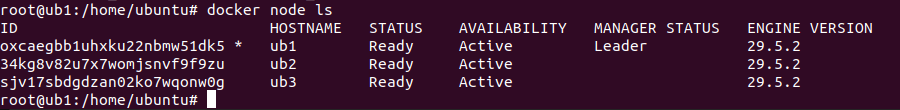
\includegraphics[width=1.05\linewidth]{../Images/docker node ls ub1 dswarm.png}
\caption{Initial replica distribution of bluesvc across the three nodes}
\label{fig:bluesvc_initial}
\end{figure}

Swarm distributed the five replicas unevenly: two were placed on \texttt{ub1}, two on \texttt{ub3}, and one on \texttt{ub2}. This distribution reflects Swarm's scheduling algorithm, which attempts to spread replicas across available nodes based on resource availability rather than strict round-robin placement.

\subsection{Self-Healing: Single Container Failure}

To evaluate Swarm's self-healing capability, the container running \texttt{bluesvc.4} on \texttt{ub2} was stopped manually to simulate a container crash:

\begin{verbatim}
docker container stop <CONTAINER_ID>
\end{verbatim}

Swarm detected the failure and immediately scheduled a replacement replica on \texttt{ub2}, as shown in Figure~\ref{fig:bluesvc_selfheal_a}. The total replica count remained at five throughout, confirming that Swarm continuously reconciles the actual state with the desired state declared at service creation.

\begin{figure}[H]
\centering
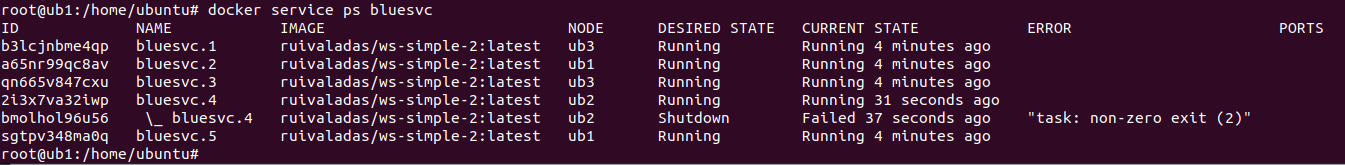
\includegraphics[width=1.05\linewidth]{../Images/docker service ps bluesvc after shut ub1.png}
\caption{Swarm scheduling a replacement for the stopped container on ub2}
\label{fig:bluesvc_selfheal_a}
\end{figure}

The stopped container was then restarted manually using \texttt{docker container start}. Inspecting the service with \texttt{docker service ps bluesvc} confirmed that the restarted container was not reabsorbed into the service: Swarm had already replaced it with a new task and tracks replicas by task identity rather than container ID. The manually restarted container continued running as an orphan outside the service.

The same test was repeated by stopping a container on \texttt{ub3}, which held two replicas. The replacement was scheduled on \texttt{ub2} rather than \texttt{ub3}, as shown in Figure~\ref{fig:bluesvc_selfheal_c}. This confirms that Swarm does not apply node affinity when rescheduling failed tasks: the replacement is placed on whichever node has available capacity, independently of where the original task was running.

\begin{figure}[H]
\centering
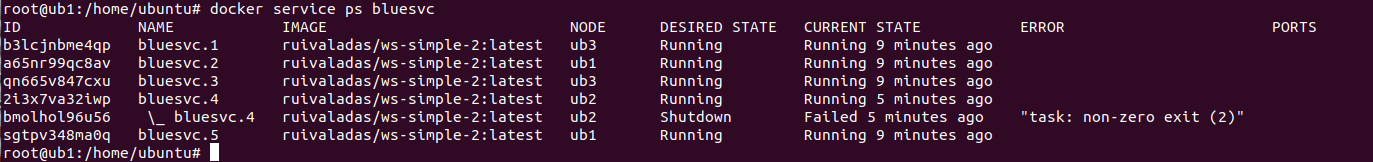
\includegraphics[width=1.05\linewidth]{../Images/docker service ps bluesvc after restart still shut.png}
\caption{Replacement container scheduled on a different node (ub2) after stopping a replica on ub3}
\label{fig:bluesvc_selfheal_c}
\end{figure}

\subsection{Self-Healing: Node Failure}

To simulate a complete node failure, \texttt{ub3} was forced to leave the Swarm:

\begin{verbatim}
docker swarm leave
\end{verbatim}

As shown in Figure~\ref{fig:bluesvc_node_failure}, \texttt{ub3} transitioned to a \texttt{Down} status in \texttt{docker node ls}, and all replicas previously assigned to it were rescheduled onto the remaining nodes (\texttt{ub1} and \texttt{ub2}). The total replica count was maintained at five. The behaviour is consistent with single container failure: in both cases Swarm detects the loss of running tasks and immediately schedules replacements to restore the desired state.

\begin{figure}[H]
\centering
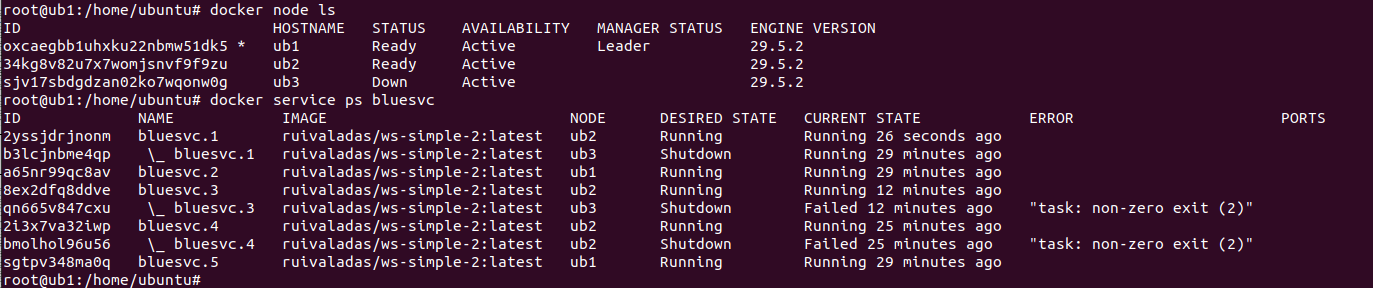
\includegraphics[width=1.05\linewidth]{../Images/node ls after ub3 left swarm.png}
\caption{Node ub3 shown as Down after leaving the Swarm, with its replicas rescheduled to ub1 and ub2}
\label{fig:bluesvc_node_failure}
\end{figure}

\subsection{Node Recovery and Rebalancing}

After \texttt{ub3} left the Swarm, it was rejoined as a worker node using the token obtained from the manager:

\begin{verbatim}
docker swarm join-token worker   # run at ub1
docker swarm join --token <TOKEN> 20.0.0.1:2377   # run at ub3
\end{verbatim}

As shown in Figure~\ref{fig:bluesvc_rejoin}, \texttt{ub3} rejoined the cluster as a new node entry (the previous \texttt{Down} entry remained visible). However, no replicas were automatically redistributed to it: all five tasks continued running on \texttt{ub1} and \texttt{ub2}. This confirms that Docker Swarm does not perform automatic rebalancing after a node recovery, in order to avoid unnecessarily disrupting running services.

\begin{figure}[H]
\centering
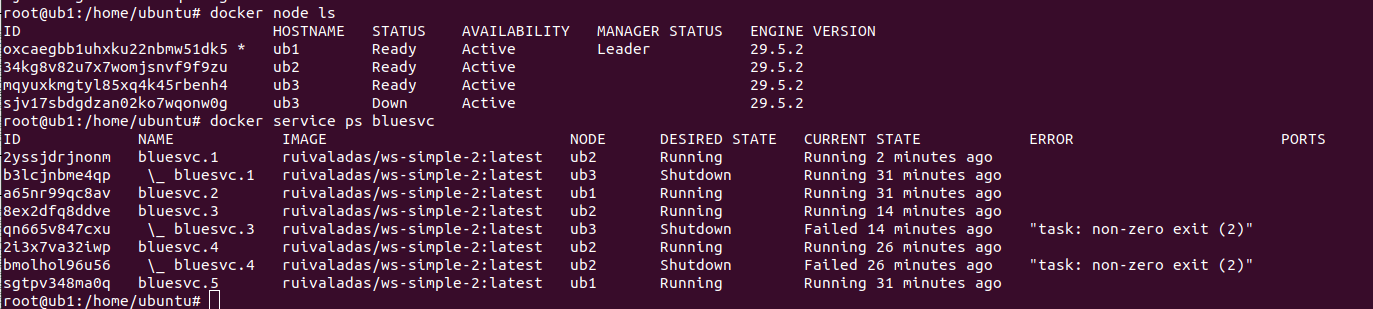
\includegraphics[width=1.05\linewidth]{../Images/node ls after ub3 rejoined swarm.png}
\caption{ub3 rejoined as a new node, with no automatic redistribution of replicas}
\label{fig:bluesvc_rejoin}
\end{figure}

To redistribute replicas across all nodes including the recovered \texttt{ub3}, a forced service update was issued at the manager:

\begin{verbatim}
docker service update --force bluesvc
\end{verbatim}

This command triggers a rolling restart of all service tasks, replacing each one sequentially. As shown in Figure~\ref{fig:bluesvc_rebalance}, Swarm used the opportunity to reschedule tasks more evenly, and \texttt{ub3} received one replica after the update completed. The output \texttt{verify: Service bluesvc converged} confirmed that all five tasks reached the running state successfully. The \texttt{--force} flag is therefore the standard mechanism to manually trigger rebalancing in Docker Swarm following node recovery.

\begin{figure}[H]
\centering
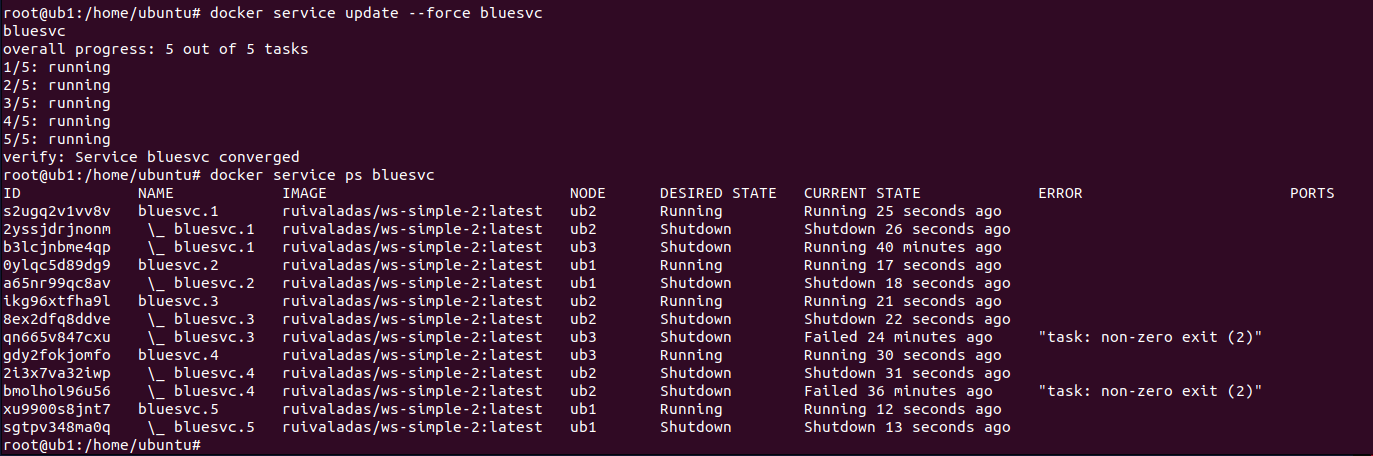
\includegraphics[width=1.05\linewidth]{../Images/1780147043317_image.png}
\caption{Forced update redistributing replicas across all three nodes including the recovered ub3}
\label{fig:bluesvc_rebalance}
\end{figure}

\subsection{Load Balancing}
 
To test the load balancing behaviour of the service, a Python client was deployed on the \texttt{saar-tools} appliance, connected to \texttt{Switch1} on the \texttt{20.0.0.0/24} subnet. The client sends a configurable number of sequential HTTP requests to the service, with a one-second interval between each, and prints the hostname returned by the server. Ten requests were directed to \texttt{ub1} on port 3000:
 
\begin{verbatim}
python3 /tmp/client.py 20.0.0.1 3000 10
\end{verbatim}
 
As shown in Figure~\ref{fig:bluesvc_loadbalance}, the five container hostnames appeared in a repeating cycle of the same fixed order across all ten responses, confirming that Docker Swarm uses a \textbf{round-robin} load balancing algorithm. Each of the five replicas was contacted exactly twice, with no deviation from the sequence.
 
\begin{figure}[H]
\centering
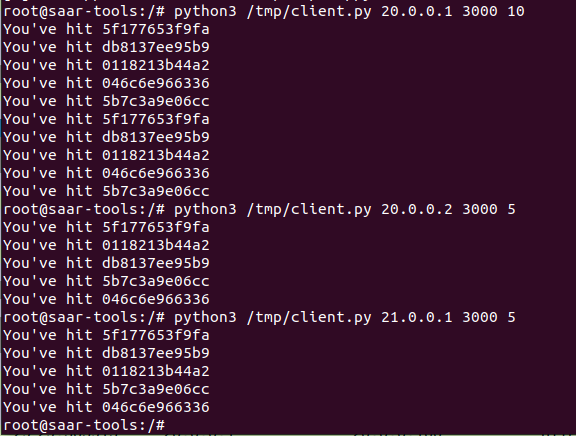
\includegraphics[width=0.75\linewidth]{../Images/script run saartools ubdswarm1.png}
\caption{Round-robin load balancing observed across 10 HTTP requests to bluesvc}
\label{fig:bluesvc_loadbalance}
\end{figure}
 
The test was repeated directing requests to \texttt{ub2} (20.0.0.2) and \texttt{ub3} (21.0.0.1) on the same port. In all cases the service responded correctly, confirming that Docker Swarm's \textbf{routing mesh} allows the service to be reached at any node's IP address, regardless of whether that node is running a replica of the service. Incoming connections are intercepted by the ingress network and forwarded to an available container transparently.
 
A Wireshark capture was performed on the link between \texttt{saar-tools} and \texttt{Switch1} to inspect the individual HTTP messages. Figure~\ref{fig:bluesvc_http_get} shows the HTTP GET request sent by the client to \texttt{20.0.0.1} on port 3000, and Figure~\ref{fig:bluesvc_http_200} shows the corresponding HTTP 200 OK response.
 
\begin{figure}[H]
\centering
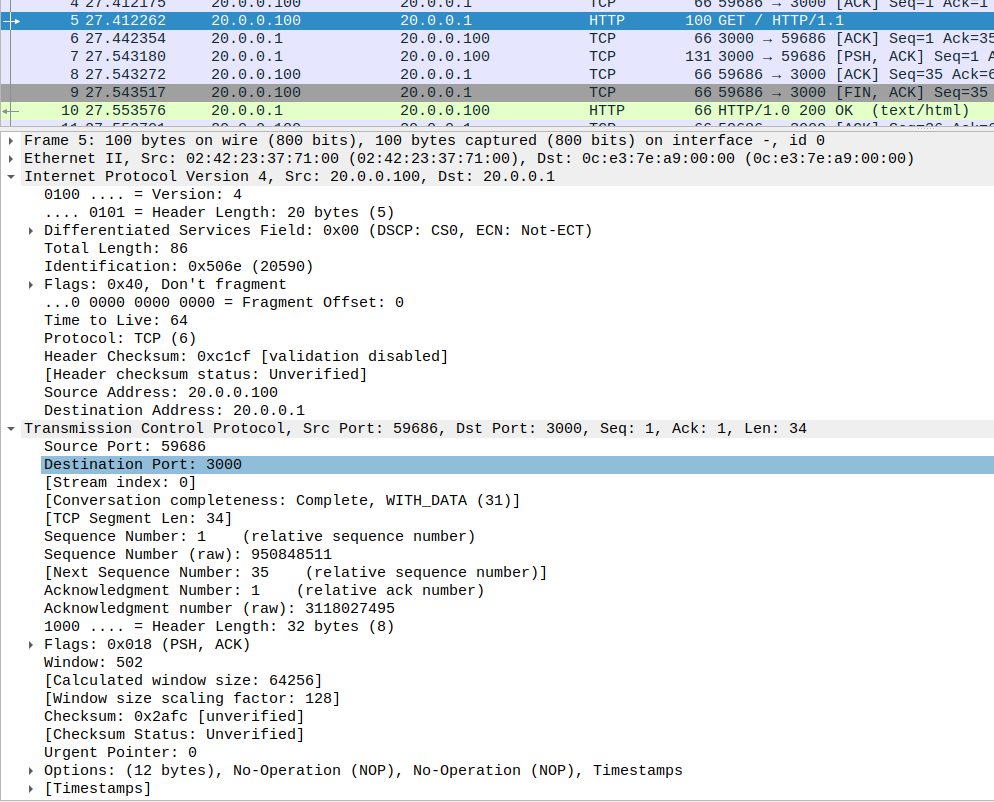
\includegraphics[width=0.9\linewidth]{../Images/7.3.3 http get.png}
\caption{HTTP GET request from saar-tools to bluesvc on port 3000}
\label{fig:bluesvc_http_get}
\end{figure}
 
\begin{figure}[H]
\centering
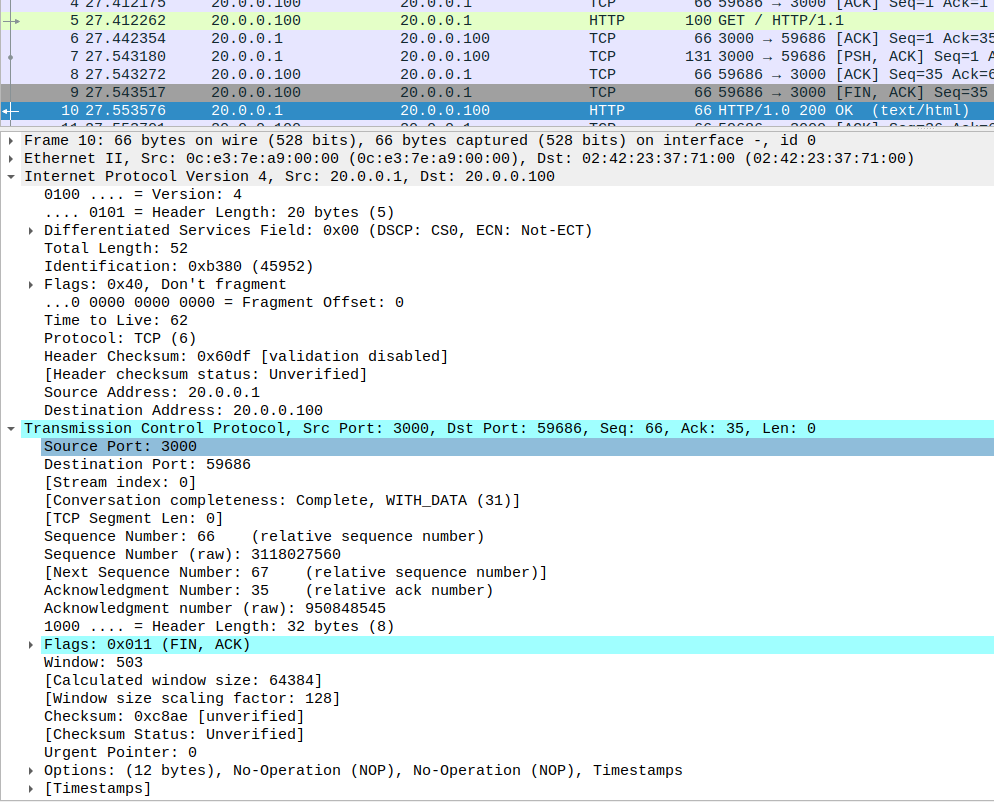
\includegraphics[width=0.9\linewidth]{../Images/7.3.3 http 200.png}
\caption{HTTP 200 OK response from bluesvc to saar-tools}
\label{fig:bluesvc_http_200}
\end{figure}
 
The capture shown in Figure~\ref{fig:bluesvc_ws_overview} confirmed that a new TCP connection was established for every HTTP request. Each request followed a complete SYN, SYN-ACK, ACK, GET, PSH/ACK, HTTP 200 OK, FIN sequence, with successive connections opening approximately one second apart.
 
\begin{figure}[H]
\centering
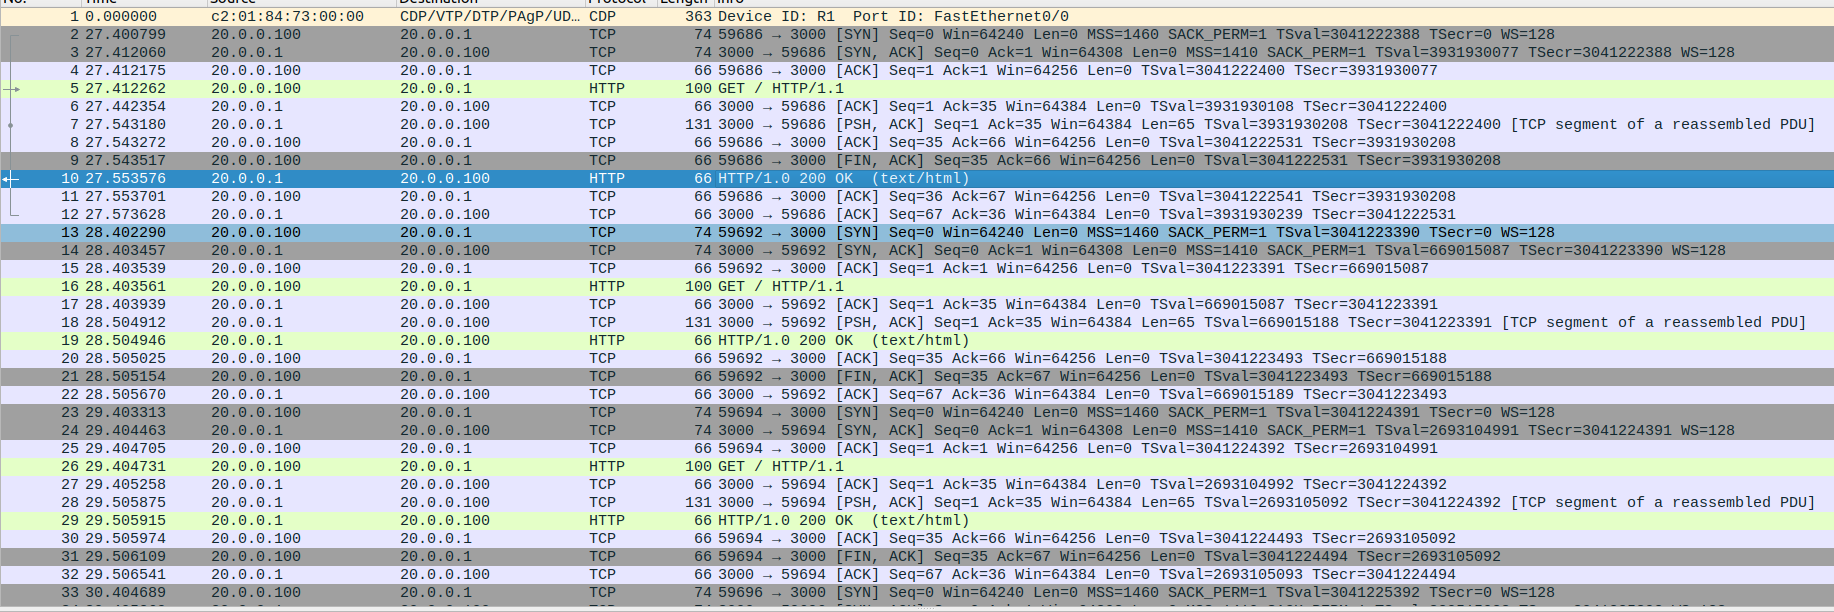
\includegraphics[width=0.95\linewidth]{../Images/7.3.3 wireshark overview.png}
\caption{Wireshark capture on the saar-tools link showing repeated TCP connection cycles}
\label{fig:bluesvc_ws_overview}
\end{figure}
 
\subsection{Service Rescaling}
 
The service was rescaled from five to three replicas using:
 
\begin{verbatim}
docker service scale bluesvc=3
\end{verbatim}
 
As shown in Figure~\ref{fig:bluesvc_scale}, Swarm immediately shut down two of the excess replicas and converged to the new desired state of three running tasks, one per node. The output \texttt{verify: Service bluesvc converged} confirmed successful rescaling.
 
\begin{figure}[H]
\centering
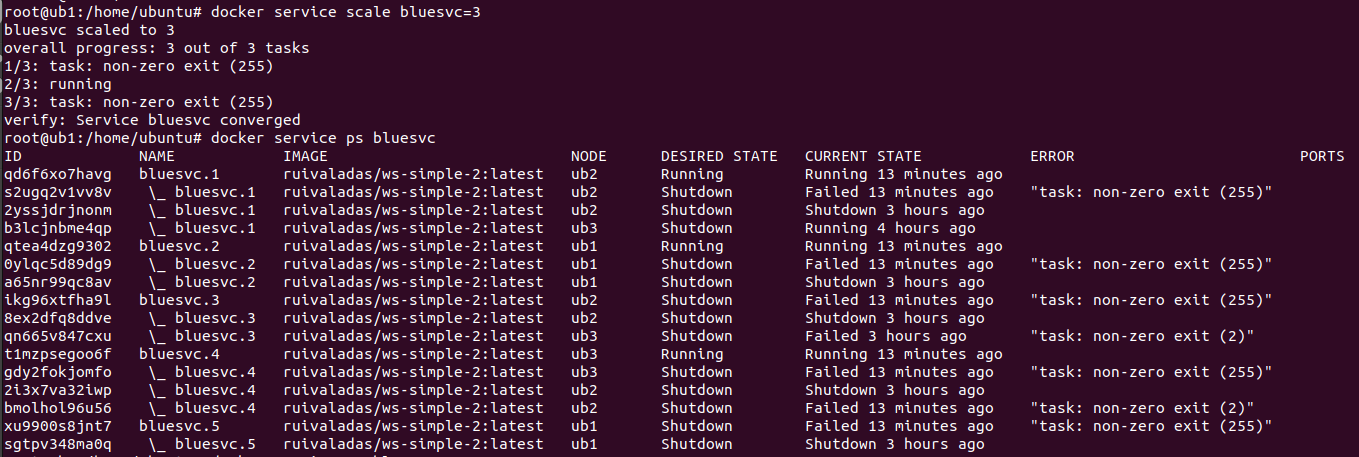
\includegraphics[width=0.9\linewidth]{../Images/7.3.4 scale down.png}
\caption{bluesvc rescaled from five to three replicas, one per node}
\label{fig:bluesvc_scale}
\end{figure}
 
Docker Swarm does not support automatic scaling based on workload natively. Achieving autoscaling would require an external solution, such as a monitoring script that periodically measures resource utilisation and issues \texttt{docker service scale} commands accordingly, or a third-party orchestration platform. Kubernetes addresses this natively through its Horizontal Pod Autoscaler (HPA), which scales deployments automatically based on observed CPU or memory metrics.
 
\subsection{Container Network Interfaces}
 
With three replicas running, one per node, the network interfaces of each container were inspected using \texttt{docker exec <CONTAINER\_ID> ip addr}. As shown in Figures~\ref{fig:ipaddr_ub1}, \ref{fig:ipaddr_ub2}, and \ref{fig:ipaddr_ub3}, each container presented three non-loopback interfaces, one more than the standalone containers of Section~7.1.
 
\begin{figure}[H]
\centering
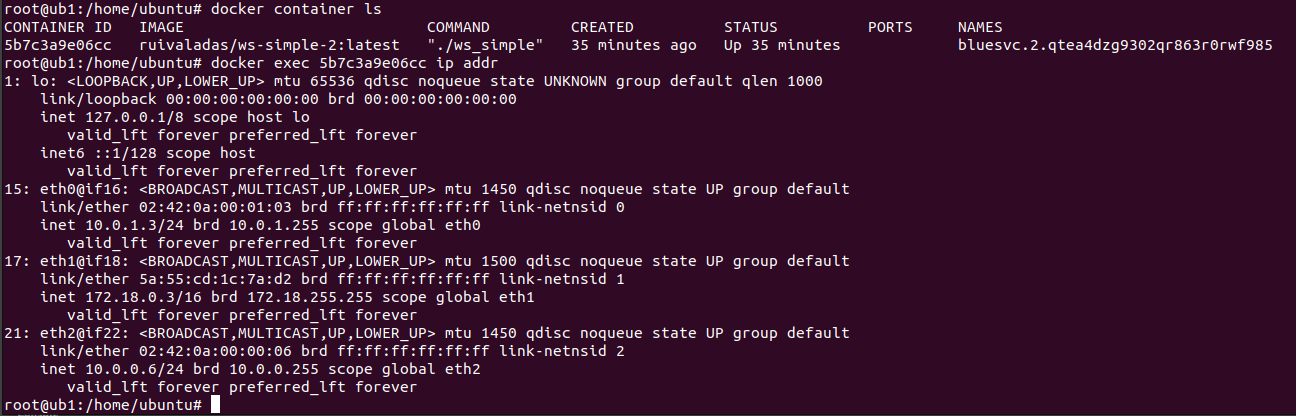
\includegraphics[width=0.9\linewidth]{../Images/7.3.5 ip addr ub1.png}
\caption{Network interfaces of the bluesvc container on ub1}
\label{fig:ipaddr_ub1}
\end{figure}
 
\begin{figure}[H]
\centering
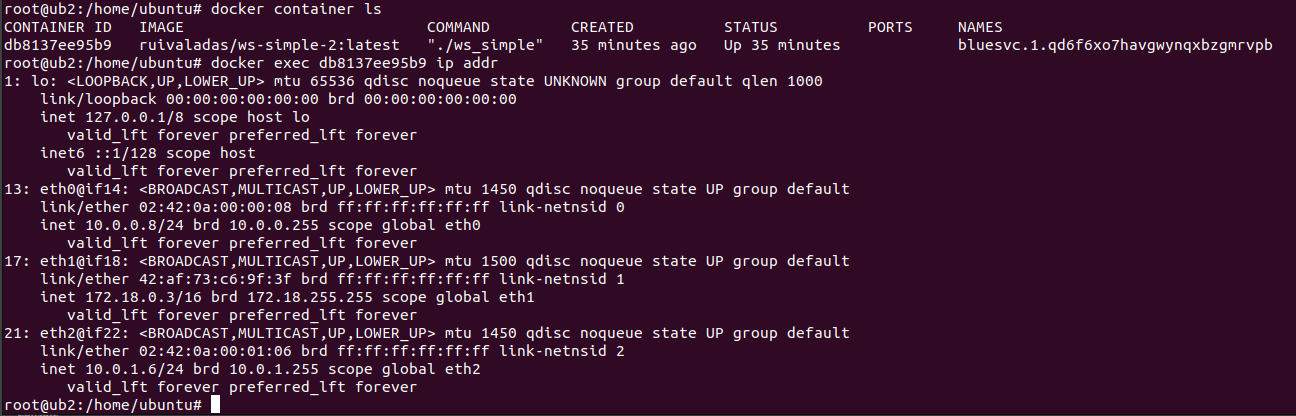
\includegraphics[width=0.9\linewidth]{../Images/7.3.5 ip addr ub2.png}
\caption{Network interfaces of the bluesvc container on ub2}
\label{fig:ipaddr_ub2}
\end{figure}
 
\begin{figure}[H]
\centering
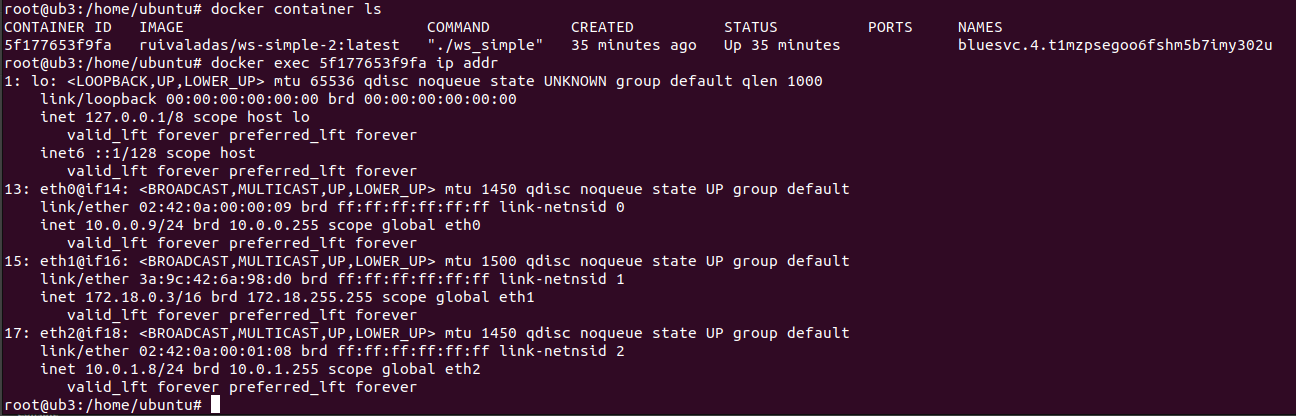
\includegraphics[width=0.9\linewidth]{../Images/7.3.5 ip addr ub3.png}
\caption{Network interfaces of the bluesvc container on ub3}
\label{fig:ipaddr_ub3}
\end{figure}
 
The three interfaces and their corresponding networks are summarised in Table~\ref{tab:container_interfaces}.
 
\begin{table}[H]
\centering
\begin{tabular}{|c|c|c|c|c|}
\hline
\textbf{Interface} & \textbf{Network} & \textbf{VNI} & \textbf{Subnet} & \textbf{Purpose} \\
\hline
eth0 & blue & 4097 & 10.0.1.0/24 & Service overlay network \\
\hline
eth1 & docker\_gwbridge & --- & 172.18.0.0/16 & Gateway to host \\
\hline
eth2 & ingress & 4096 & 10.0.0.0/24 & Swarm routing mesh \\
\hline
\end{tabular}
\caption{Network interfaces of bluesvc service containers}
\label{tab:container_interfaces}
\end{table}
 
The \texttt{eth0} interface connects the container to the \texttt{blue} overlay network (VNI 4097), used for direct container-to-container communication within the service. The \texttt{eth1} interface connects to the \texttt{docker\_gwbridge} local bridge (172.18.0.0/16), which provides the container with a gateway to the host for outbound traffic. The \texttt{eth2} interface connects to the \texttt{ingress} overlay network (VNI 4096), which implements the Swarm routing mesh and handles externally published traffic arriving on port 3000.
 
This additional interface, absent in the standalone containers of Section~7.1, is the key structural difference between service containers and standalone containers in Docker Swarm: service containers are always attached to the shared ingress network to participate in the routing mesh.
 
\subsection{HTTP Request Path and VXLAN Encapsulation}
 
To trace the path followed by HTTP requests through the Swarm infrastructure, a Wireshark capture was started on the \texttt{ens3} interface of \texttt{ub1} and three HTTP requests were sent from \texttt{saar-tools} to \texttt{ub1} on port 3000. The capture, filtered by HTTP, is shown in Figure~\ref{fig:bluesvc_http_overview}.
 
\begin{figure}[H]
\centering
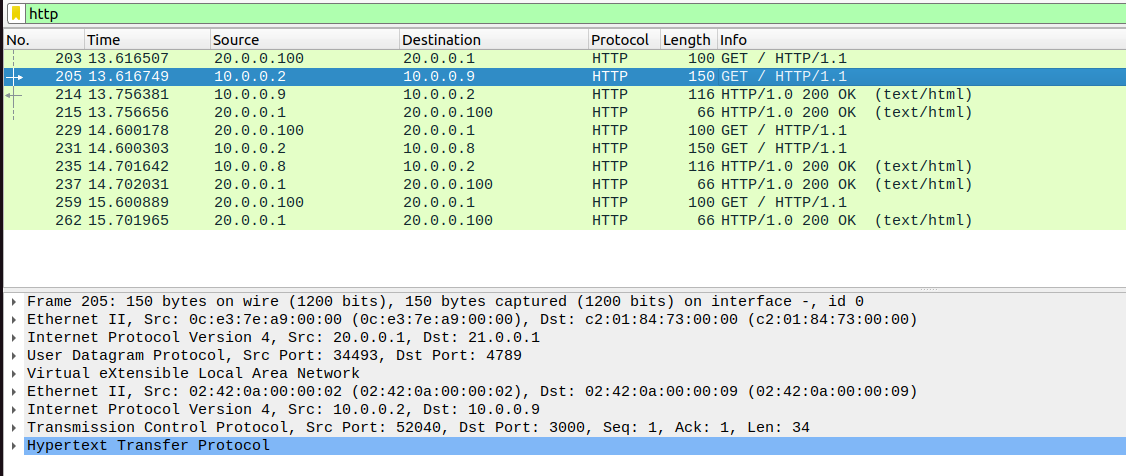
\includegraphics[width=0.95\linewidth]{../Images/7.3.6 wireshark overview.png}
\caption{HTTP traffic captured on ub1's ens3 interface during three client requests}
\label{fig:bluesvc_http_overview}
\end{figure}
 
Two distinct forwarding paths were observed depending on whether the selected container was local or remote.
 
\paragraph{Container on ub1 (local).} When the routing mesh selected the local replica, the HTTP GET arrived directly from \texttt{saar-tools} (20.0.0.100) to \texttt{ub1} (20.0.0.1) at the physical layer, as shown in Figure~\ref{fig:bluesvc_http_direct}. The response was returned directly from \texttt{ub1} to \texttt{saar-tools} without any tunnelling. No VXLAN packets were generated.
 
\begin{figure}[H]
\centering
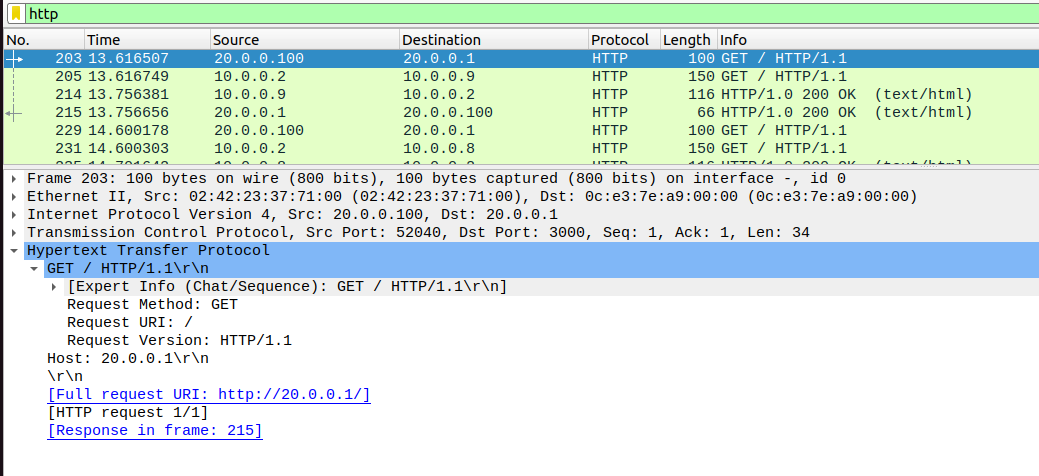
\includegraphics[width=0.9\linewidth]{../Images/7.3.6 http direct.png}
\caption{Direct HTTP exchange when the selected container is on the contacted node (ub1)}
\label{fig:bluesvc_http_direct}
\end{figure}
 
\paragraph{Container on a remote node (ub2 or ub3).} When the routing mesh selected a replica on a different node, \texttt{ub1} encapsulated the request in a VXLAN tunnel and forwarded it to the appropriate remote node. The packet detail for a request forwarded to \texttt{ub3} is shown in Figure~\ref{fig:bluesvc_vxlan_detail}.
 
\begin{figure}[H]
\centering
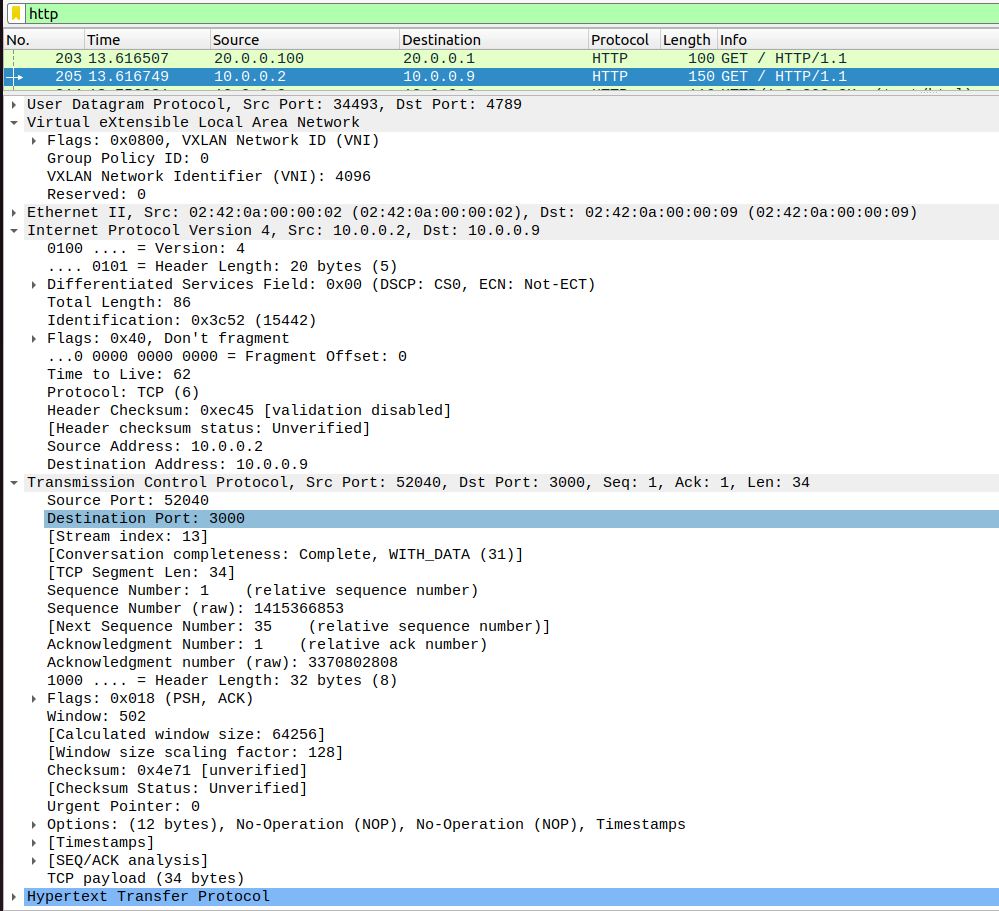
\includegraphics[width=0.9\linewidth]{../Images/7.3.6 vxlan tunnelled.png}
\caption{VXLAN encapsulation of an HTTP request forwarded from ub1 to ub3}
\label{fig:bluesvc_vxlan_detail}
\end{figure}
 
The encapsulation structure was as follows. The outer IP header carried the physical node addresses (\texttt{20.0.0.1} $\rightarrow$ \texttt{21.0.0.1}), routing the packet across the underlay network via \texttt{R1}. The UDP destination port was 4789 (the standard VXLAN port). The VXLAN header identified the tunnel with \textbf{VNI 4096}, corresponding to the ingress network. The inner Ethernet frame carried the ingress network MAC addresses (\texttt{02:42:0a:00:00:02} $\rightarrow$ \texttt{02:42:0a:00:00:09}), and the inner IP header carried the ingress network addresses (\texttt{10.0.0.2} $\rightarrow$ \texttt{10.0.0.9}). The inner TCP segment was addressed to port 3000.
 
The response from the remote container followed the reverse path: the remote node encapsulated the HTTP 200 OK in a VXLAN packet back to \texttt{ub1}, which decapsulated it and forwarded the response to \texttt{saar-tools}. From the client's perspective, the entire exchange appeared as a direct conversation with \texttt{ub1}.
 
The VXLAN filter view in Figure~\ref{fig:bluesvc_vxlan_filter} shows the full sequence of tunnelled exchanges, confirming that two of the three requests required inter-node tunnelling (to \texttt{ub3} and \texttt{ub2} respectively), while the third was served locally.
 
\begin{figure}[H]
\centering
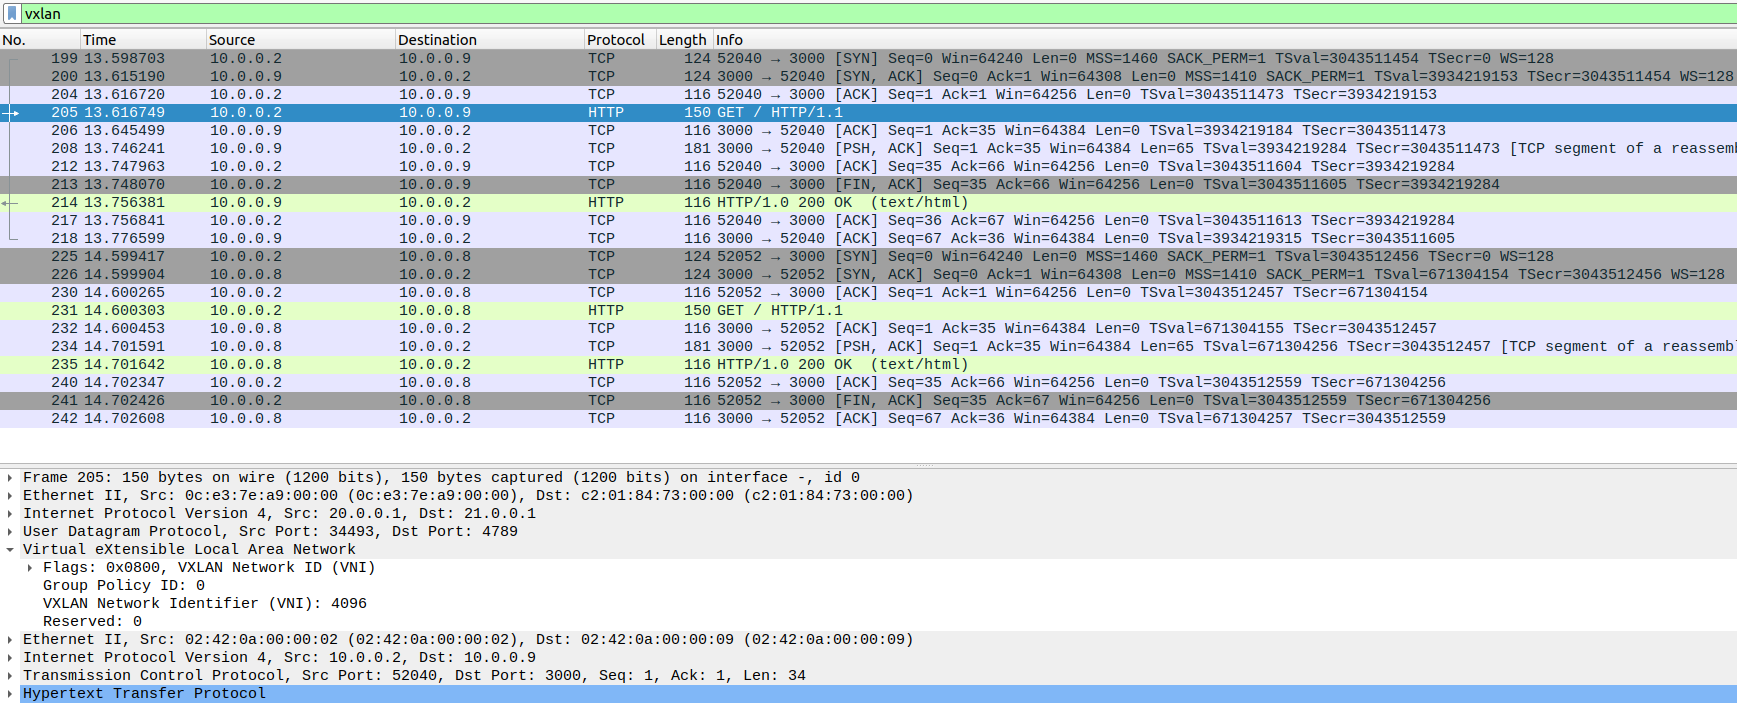
\includegraphics[width=0.95\linewidth]{../Images/7.3.6 vxlan filter.png}
\caption{VXLAN-filtered capture showing tunnelled HTTP exchanges to remote nodes}
\label{fig:bluesvc_vxlan_filter}
\end{figure}
 
\subsection{Comparison with a Second Service: redsvc}
 
A second service, \texttt{redsvc}, was created on the \texttt{red} overlay network with three replicas and external access on port 3001:
 
\begin{verbatim}
docker service create --network red --name redsvc \
    --replicas 3 --publish 3001:80 ruivaladas/ws-simple-2
\end{verbatim}
 
As shown in Figure~\ref{fig:redsvc_ps}, Swarm distributed one replica per node, mirroring the \texttt{bluesvc} distribution.
 
\begin{figure}[H]
\centering
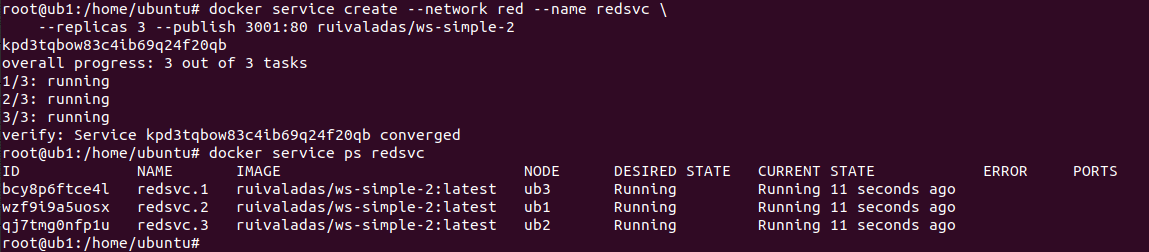
\includegraphics[width=0.9\linewidth]{../Images/7.3.7 redsvc ps.png}
\caption{Replica distribution of redsvc across the three nodes}
\label{fig:redsvc_ps}
\end{figure}
 
A new Wireshark capture was performed while sending three HTTP requests to \texttt{ub1} on port 3001. The packet detail of a tunnelled request, shown in Figure~\ref{fig:redsvc_vxlan}, revealed that the VXLAN VNI used was again \textbf{4096} — identical to \texttt{bluesvc}.
 
\begin{figure}[H]
\centering
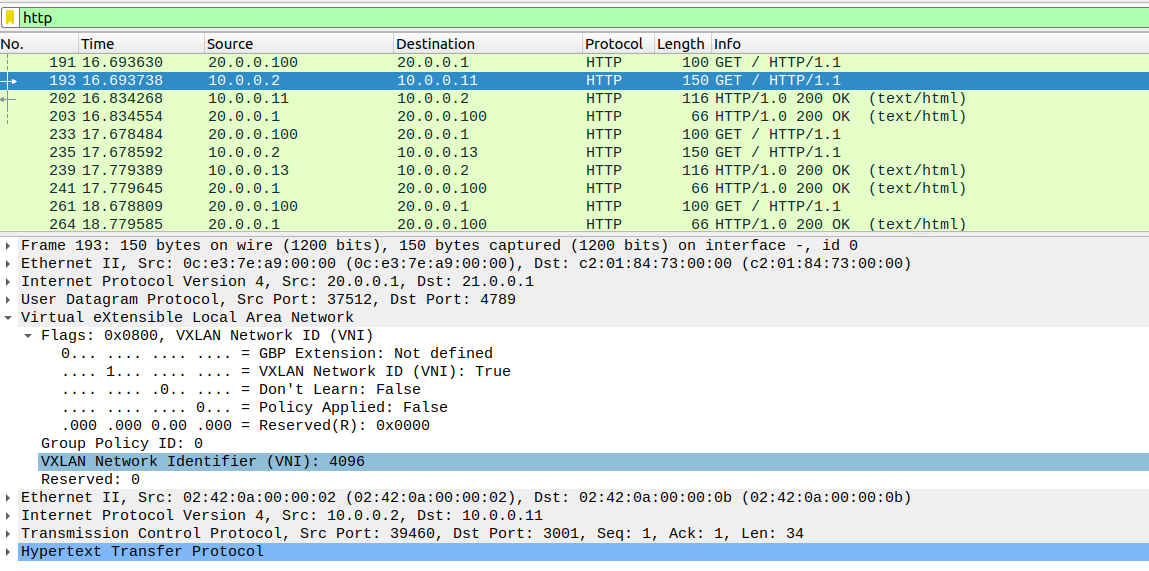
\includegraphics[width=0.95\linewidth]{../Images/7.3.7 vxlan redsvc.png}
\caption{VXLAN encapsulation of an HTTP request for redsvc, showing VNI 4096}
\label{fig:redsvc_vxlan}
\end{figure}
 
This confirms that the ingress network is \textbf{shared across all Swarm services}, regardless of which user-defined overlay network (blue or red) the service is attached to. The VNI 4096 tunnel is used for all externally published traffic in the Swarm, and the destination port in the inner TCP header (3000 or 3001) is what distinguishes traffic belonging to different services within the shared ingress tunnel. The \texttt{blue} and \texttt{red} overlay networks (VNI 4097 and 4098 respectively) are used exclusively for direct container-to-container communication within each service, and are not involved in handling external client requests.

\subsection{Comparison with AI Tool Explanation}
 
The behaviour observed experimentally is consistent with the explanation provided by the AI tool consulted during the preparation of this exercise. The AI correctly described Docker Swarm services as a declarative abstraction over replicated containers, identified the ingress network and routing mesh as the mechanism behind load balancing and external accessibility, and explained that self-healing operates by reconciling actual state with desired state without node affinity.
 
Two points of nuance emerged from the experiments that the AI description addressed only partially. First, the AI noted that Swarm does not rebalance automatically after node recovery, which was confirmed: after \texttt{ub3} rejoined the cluster, no replicas were redistributed until a forced update was issued with \texttt{docker service update --force}. Second, the AI correctly identified round-robin as the load balancing algorithm, which the Wireshark and client output confirmed precisely. The experimental captures added concrete detail to the AI explanation by showing the actual VNI values, inner and outer IP and MAC address pairs, and the exact packet structure of the VXLAN tunnels used by the ingress network.

\end{document}